\documentclass[12pt, a4paper, oneside, openright]{book}
\usepackage[vcentering, dvips, a4paper, top=2cm, bottom=2cm, left=3cm, right=1.75cm]{geometry}
\usepackage{hyperref}%for cross references
\usepackage[utf8]{inputenc}
\usepackage{fontspec}

\usepackage{polyglossia}
\setdefaultlanguage{latvian}
\usepackage{fixlatvian}

\usepackage{setspace}
  \onehalfspacing % to have 1.5 space between lines

\usepackage{indentfirst}
\usepackage[nonumberlist]{glossaries}
\usepackage{amsfonts} %includes a list of mathematical symbols and styles. Useful if you are using equations a lot
\usepackage{amsmath}
\usepackage{graphicx}
\usepackage{psfrag} %I use eps files for my pictures, and with this package I can replace text in those images. This allows me to have the same font size and type in both images and text.
%\usepackage{tipa}
%\usepackage{textcomp}
\usepackage{layout} %simple package, which prints an overview of all the margins on the page when you insert \layout.
\usepackage{appendix} %allows more detailed control over appendicies.

\usepackage[numbers, sort]{natbib}  %powerful extension for controlling your references.
  \bibliographystyle{siam}

\usepackage{parskip}
\usepackage{fancyhdr} %this package allows control over the headers and footers for documents with class book. The use is non-trivial, but powerful results are possible.
\usepackage{acronym}%for using acronym and building a list of acronym
\usepackage{multirow}
\usepackage{enumitem}
  \setlist{topsep=0pt, parsep=0pt, itemsep=0pt}

\usepackage{pdfpages} %to include PDF files


% Redefine plain page style
\fancypagestyle{plain}{
  \fancyhf{}
  \renewcommand{\headrulewidth}{0pt}
  \fancyfoot[RO]{\thepage} %add LE for duplex

}

% Code for creating empty pages
% No headers on empty pages before new chapter
\makeatletter
\def\cleardoublepage{\clearpage\if@twoside \ifodd\c@page\else
    \hbox{}
    \thispagestyle{plain}
    \newpage
    \if@twocolumn\hbox{}\newpage\fi\fi\fi}
\makeatother \clearpage{\pagestyle{plain}\cleardoublepage}

% Define pagestyle
\pagestyle{fancy}
\fancyhf{}
\renewcommand{\chaptermark}[1]{\markboth{ \emph{#1}}{}}
\fancyhead[LO]{\leftmark}
%\fancyhead[RE]{\leftmark} %required for duplex
\fancyfoot[RO]{\thepage} %add LE for duplex

%For titlepage
\newcommand{\HRule}{\rule{\linewidth}{0.3mm}}


% This is all for formatting and making the Table of Contents according to
% spec. Don't play with it.
\makeatletter
\renewcommand*\l@chapter[2]{%
  \ifnum \c@tocdepth >\m@ne
    \addpenalty{-\@highpenalty}%
    \vskip 1.0em \@plus\p@
    \setlength\@tempdima{1.5em}%
    \begingroup
      \parindent \z@ \rightskip \@pnumwidth
      \parfillskip -\@pnumwidth
      \leavevmode \bfseries
      \advance\leftskip\@tempdima
      \hskip -\leftskip
      #1\nobreak\normalfont\leaders\hbox{$\m@th
        \mkern \@dotsep mu\hbox{.}\mkern \@dotsep
        mu$}\hfill\nobreak\hb@xt@\@pnumwidth{\hss #2}\par
      \penalty\@highpenalty
    \endgroup
  \fi}
\makeatother

% TOC display levels: Chapter, Section, subsection
\setcounter{tocdepth}{2}


%Create Glossary
\makeglossaries
\loadglsentries{burti}


%To remove the word ``Chapter'' before Chapter #
\usepackage{titlesec}
\titleformat{\chapter}[hang]{\bf\huge}{\thechapter}{2pc}{}

%To dedicate the work to someone
\newenvironment{dedication}
{
   \cleardoublepage
   \thispagestyle{empty}
   \vspace*{\stretch{1}}
   \hfill\begin{minipage}[t]{0.66\textwidth}
   \raggedright
}%
{
   \end{minipage}
   \vspace*{\stretch{3}}
   \clearpage
}

%fixing \headhight error
\setlength{\headheight}{15pt}

%FOR MATLAB CODE LISTING
\usepackage{listings}
\usepackage[usenames,dvipsnames]{color}
% This is the color used for MATLAB comments below
\definecolor{MyDarkGreen}{rgb}{0.0,0.4,0.0}

% For faster processing, load Matlab syntax for listings
\lstloadlanguages{Matlab}%
\lstset{language=Matlab,                        % Use MATLAB
        frame=single,                           % Single frame around code
        basicstyle=\small\ttfamily,             % Use small true type font
        keywordstyle=[1]\color{Blue}\bf,        % MATLAB functions bold and blue
        keywordstyle=[2]\color{Purple},         % MATLAB function arguments purple
        keywordstyle=[3]\color{Blue}\underbar,  % User functions underlined and blue
        identifierstyle=,                       % Nothing special about identifiers
                                                % Comments small dark green courier
        commentstyle=\usefont{T1}{pcr}{m}{sl}\color{MyDarkGreen}\small,
        stringstyle=\color{Purple},             % Strings are purple
        showstringspaces=false,                 % Don't put marks in string spaces
        tabsize=5,                              % 5 spaces per tab
        %
        %%% Put standard MATLAB functions not included in the default
        %%% language here
        morekeywords={xlim,ylim,var,alpha,factorial,poissrnd,normpdf,normcdf},
        %
        %%% Put MATLAB function parameters here
        morekeywords=[2]{on, off, interp},
        %
        %%% Put user defined functions here
        morekeywords=[3]{FindESS, homework_example},
        %
        morecomment=[l][\color{Blue}]{...},     % Line continuation (...) like blue comment
        numbers=left,                           % Line numbers on left
        firstnumber=1,                          % Line numbers start with line 1
        numberstyle=\tiny\color{Blue},          % Line numbers are blue
        stepnumber=5                            % Line numbers go in steps of 5
        }
% Includes a MATLAB script.
% The first parameter is the label, which also is the name of the script
%   without the .m.
% The second parameter is the optional caption.
\newcommand{\matlabscript}[2]
  {\begin{itemize}\item[]\lstinputlisting[caption=#2,label=#1]{#1.m}\end{itemize}}
%%%%%%%%%%%%%%%%%%%%%%%%%%%%%%%%%%%%%FOR MATLAB CODE%%%%%%%%%%%%%%%%%%%%%%%%%%%%%%%%%%%%%%


%%%%%%%%%%%%%%%%%%%%%%%%%%%%%%%%%%%%%%%%%%%%%%%%%%%%%%%%%%%%%%%%Here begin my document%%%%%%%%%%%%%%%%%%%%%%%%%%%%%%%%%%%%%%%
\begin{document}
\frontmatter %page numbering in LATIN LETTERS
\pagenumbering{arabic}
\begin{titlepage}

\begin{center}
\renewcommand{\baselinestretch}{1.00}\normalsize
% Upper part of the page
%\includegraphics[width=0.15\textwidth]{./logo}\\[1cm]

\textsc{\LARGE rīgas tehniskā universitāte\\
\normalsize{Elektronikas un telekomunikāciju fakultāte}\\[0.18cm]
\LARGE telekomunikāciju institūts}\\[5.5cm]




% Title
\HRule \\[0.4cm]
{ \Large \bfseries {Mobilitātes ietekme uz pakalpojuma kvalitāti sensoru tīklos}\\
 \small angļu valodā "Impact of Mobility on QoS in Sensor Networks"}\\[0.4cm]
\HRule \\[0.6cm]

\textsc{\normalsize Maģistra darbs}\\[6.5cm]

% Author and supervisor
\begin{minipage}[b]{0.47\linewidth}
\begin{flushleft} \large
\emph{Autors:}\\
Olga \textsc{Dmitričenko}\\
\small{Telekomunikāciju studiju programmas\\
maģistrante\\
maģ. apl. nr. 021REB094}\\
\end{flushleft}
\end{minipage}
\begin{minipage}[b]{0.5\linewidth}
\begin{flushright} \large
\emph{Zinātniskais vadītājs:} \\
prof. Gunārs \textsc{Lauks}, Dr.Sc.Ing.\\
\end{flushright}
\end{minipage}
\vspace{3.0cm}


% Bottom of the page
{\large Rīga, 2012}

\end{center}

\end{titlepage}
%DEDICATION%%
\begin{dedication}
\textit{Veltīts\\ Anatolijai un Sergejam}
\end{dedication}
\clearpage{\pagestyle{empty}\cleardoublepage}

%%NOVERTEJUMA LAPPA%%
\phantomsection
\addcontentsline{toc}{chapter}{Maģistra darba novērtējuma lapa}
\includepdfset{pages=-,pagecommand=\thispagestyle{empty}}
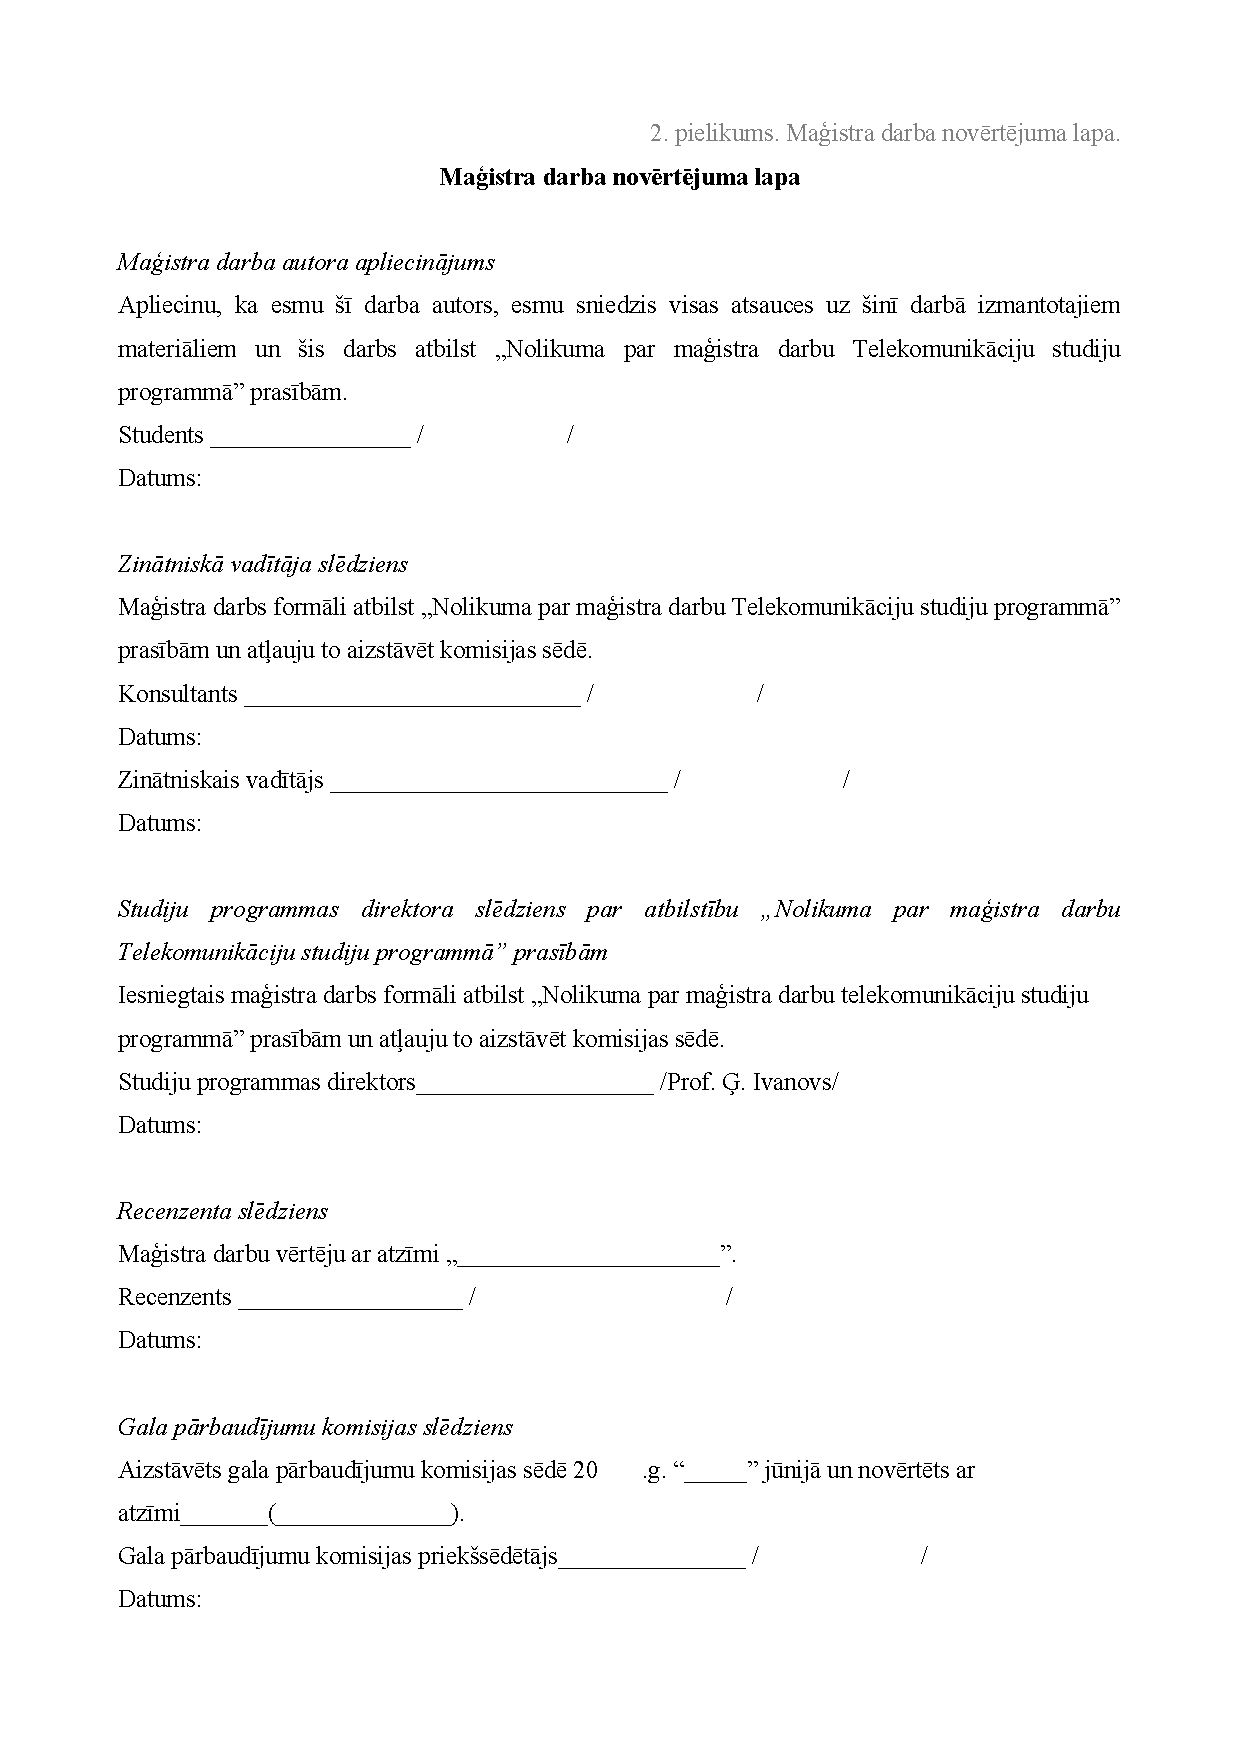
\includepdf{./pdf/novert.pdf}
\clearpage{\pagestyle{empty}\cleardoublepage}

%%ORTUS%%
\phantomsection
\addcontentsline{toc}{chapter}{Studiju noslēguma darba autora apliecinājums}
\includepdfset{pages=-,pagecommand=\thispagestyle{empty}}
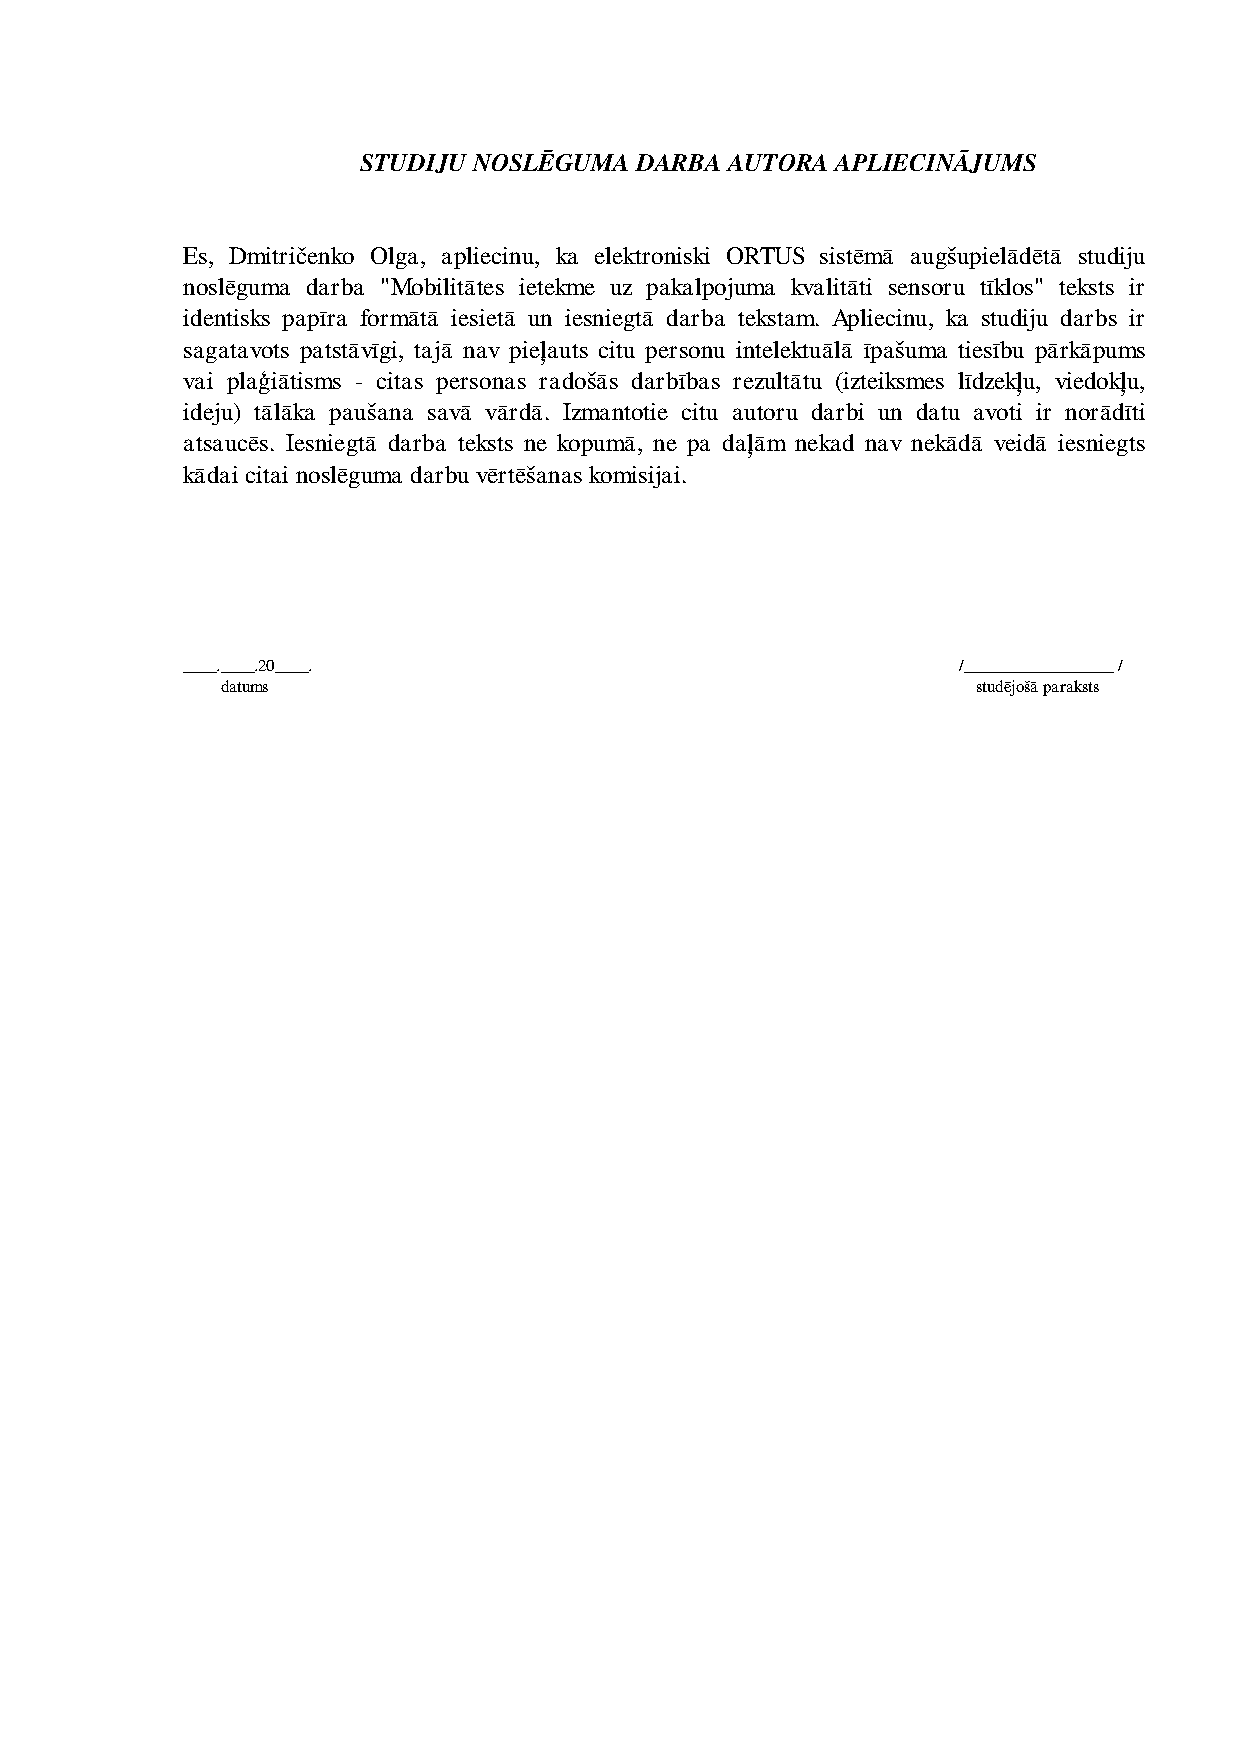
\includepdf{./pdf/ortus1.pdf}


%%ANNOTACIJAS%%
  \chapter{Anotācija}

Maģistra darba pētījuma mērķis ir izpētīt mobilitātes ietekmi uz bitu kļūdu intensitāti (BER) bezvadu sensoru tīklos (WSN), un uzlabot WSN maršrutā izvēli ar SP-BER balstīto maršruta izvēles shēmu.
Darba pirmā daļa ir veltīta WSN infrastruktūras un tīklā notiekošo procesu izpētei. Tiek sniegta galveno WSN processu matemātiskā analīze, nodrošinot iespēju aprēķināt BER savienojuma posmā, BER daudzposma maršrutā, interferences līmeni WSN tīklā, kā arī daudzposma maršruta garumu izmaņas atkarībā no izmantotā rezervēšanas (RB) vai bez-rezervēšanas (NRBS) komutācijas risinājuma. Aprakstītie matemātiskie aprēķini var būt pielietoti jebkurai no ekspromta tīkla topoloģijas analīzei. Noslēdzot šo daļu ar ekspromta tīkla  maršrutēšanas protokolu izpēti, noslēgumā aprakstot jauno SP-BER balstīto maršruta izvēles algoritmu.

Maģistra darba pēdējā nodaļā tiek veikta WSN simulācija izmantojot AODV un DSR protokolus NS-2 vidē salīdzinot tās efektivitāti mobilitātes apstākļos ar sekojošiem parametriem paketes piegādes sadale, paketes vidējo aizkavi tīklā un caurlaidspēju. Nodaļa sniedz ieskatu mobilos WSN tīklos, kā arī apskata ar mobilitāti saistītās problēmas un to risinājumus.

Maģistra darbs ir izstrādāts saskaņā ar Rīgas Tehniskās Universitātes (RTU) Maģistra darbu izstrādes prasībām un nekādā veidā nav pretrunā ar autortiesībām. Maģistra darbā ir iekļauts 32 attēls, 5 tabulas, 25 vienādojumi un 41 atsauces uz izmantotās literatūras avotiem. Maģistra darba kopējais apjoms, iekļaujot 3 pielikumus, sastāda 77 lapas puses.
  \chapter{Annotation}
The purpose of this research is to identify an impact of mobility on the Quality of Services (QoS) in the Wireless Sensor Networks (WSN).

The first part of the project involves an evaluation of the WSN infrastructure and the processes in it, through reviewing the already existing studies in this area.  At the end of the first part the model which gives a mathematical analysis of the main WSN processes and allows to calculate BERlink and BERroute , interference in the channel, also routes the length depending on the RB or NRBS switching techniques is being explained. The calculations obtained in this part can be applied to any Ad Hoc network.In the second part the overview of the WSN switching protocols is being made and the new SP-BER–based algorith is being proposed in order to improve the switching in the WSN system.

The final part involves the simulation of the WSN with the AODV and DSR switching protocol in NS-2 and compares its performance with following metrices PDF, average network delay, network throughput. The above-mentioned approach will allow to get the better overview of the WSN and have the insight view into the problems related to node mobility.

This master thesis is aligned with formal demands of Riga’s Technical University (RTU) for the Master Thesis and does not violate any copyrights. The thesis contains 32 figures, 5 tables, 25 equations and 41 sources of information. The total volume of the thesis is 77 page, including 3 appendices.
%%SAISINAJUMU%%
  \chapter{Saīsinājumu saraksts}
\begin{acronym}
%%%A%%%
\acro{Ad Hoc}   {\acroextra{\emph{ - Ad hoc - }}Ekspromta tīkls}
\acro{AODV}     {\acroextra{\emph{ - Ad Hoc On-Demand Distance Vector Routing - }}Ekspromta tīkla pēc pieprasījuma distances vektora protokols}
\acro{AWGN}	{\acroextra{\emph{ - Additive white Gaussian Noise - }}Aditīvs baltais Gausa troksnis}
%%%B%%%
\acro{BER}      {\acroextra{\emph{ - Bit Error Rate - }}Bitu kļūdu intensitāte}
\acro{BPSK}		{\acroextra{\emph{ - Binary Phase Shift Keying - }}Binārā fāzes manipulācija}
\acro{broadcast} {acroextra{ - }Apraide}
%%%C%%%
\acro{CBR}      {\acroextra{\emph{ - Constant Bit Rate - }}Konstants bitu ātrums}
\acro{CCDF}     {\acroextra{\emph{ - Complementary Cumulative Distribution Function - }} Absolūti nepārtraukts sadalījums}
\acro{CSMA/CA}	{\acroextra{\emph{ - Carrier sense, Multiple access/Collision avoidance - }}Nesēja jušanas un sadursmju nepieļaušanas daudzpiekļuve}
%%%D%%%
\acro{DSDV}     {\acroextra{\emph{ - Destination-Sequenced Distance-Vector - }}Galamērķa secīgā distances vektora protokols}
\acro{DSR}      {\acroextra{\emph{ - Dynamic Source Routing - }}Dinamiska avota maršrutēšana }
\acro{DSSS}	{\acroextra{\emph{ - Direct Sequence Spread Spectrum - }}Tiešās secības spektra paplašināšana}
%%%F%%%
\acro{FHSS}	{\acroextra{\emph{ - Frequency-Hopping Spread Spectrum - }}Frekvences lēkāšana}
%%%G%%%
\acro{GUID}	{\acroextra{\emph{ - Globally Unique Identifier  - }}Vispārēji unikāls identifikators}
%%%I%%%
\acro{IHWN}	{\acroextra{\emph{ - Intergrated Heterogenus Wireless Network - }}Integrēts heterogēnu bezvadu tīkls}
\acro{iid}      {\acroextra{\emph{ - Independent and identically distributed - }}Neatkarīgi un viendabīgi izkliedēti}
\acro{INI}      {\acroextra{\emph{ - Inter Node Interference - }}Mezglu savstarpējie traucējumi}
%%%L%%%
\acro{LAN}      {\acroextra{\emph{ - Local Area Network - }}Lokālais tīkls}
\acro{LR-WPAN}	{\acroextra{\emph{ - Low-Rate Wireless Personal Area Networks - }}Zemo-ātrumu bezvadu personālā apgabala tīkls}
\acro{LSRP}	{\acroextra{\emph{ - Link State Routing Protocol - }}Posma stāvokļa maršrutēšanas protokols}
%%%M%%%
\acro{MAC}      {\acroextra{\emph{ - Medium Access Control - }}Vides piekļuves vadības protokols}
\acro{MAN}	{\acroextra{\emph{ - Metropolitan Area Network - }}Pilsēttīkls}
\acro{MANET}    {\acroextra{\emph{ - Mobile Ad Hoc Network - }}Mobilais ekspromta tīkls}
\acro{MPR}      {\acroextra{\emph{ - Multi Point Relay - }}Vairākstāvokļu relejs}
\acro{multicast}{\acroextra{ - }Multiraide}
%%%N%%%
\acro{NRBS}     {\acroextra{\emph{ - Nonreservation-based switching - }}Bez-rezervēšanas komutācija}
\acro{NS-2}	{\acroextra{ - }Network Simulator 2}
%%%O%%%
\acro{OFDM}	{\acroextra{\emph{ - Orthogonal Frequency Division Multiplexing - }}Ortogonālā frekvenčdales multipleksēšana }
\acro{OLSR}     {\acroextra{\emph{ - Optimized link state routing protocol - }}Optimizēts posma stāvokļa maršrutēšanas protokols}
\acro{OMM}      {\acroextra{\emph{ - Obstacle Mobility Model - }}Šķēršļu mobilitātes modelis}
\acro{ONRBS}    {\acroextra{\emph{ - Opportunistic Nonereservation-based switching - }}Oportūnistiska bez rezervēšanas komutācija }
\acro{OSI}      {\acroextra{\emph{ - Open Systems Interconnection - }}Atvērto sistēmu starpsavienojums}
%%%P%%%
\acro{PER}	{\acroextra{\emph{ - Packer Error Rate - }}Pakešu kļūdu intensitāte}
\acro{PDF}      {\acroextra{\emph{ - Packet Delivery Fraction - }}Paketes piegādes sadale}
%%%R%%%
\acro{RBS}       {\acroextra{\emph{ - Reservation-based switching - }}Rezervēšanas komutācija }
\acro{RESGO}    {\acroextra{\emph{ - Reserve-and-Go MAC - }}Rezervē un strādā MAC protokols}
\acro{RREP}     {\acroextra{\emph{ - Route Reply - }}Maršruta atbildes pakete}
\acro{RERR}     {\acroextra{\emph{ - Route Request ERROR - }}Maršruta pieprasījuma ERROR pakete}
\acro{RREQ}     {\acroextra{\emph{ - Route Request - }}Maršruta pieprasījuma pakete}
\acro{RDMM}     {\acroextra{\emph{ - Random Direction Mobility model - }}Gadījuma virzienu mobilitātes modelis}
\acro{RWM}      {\acroextra{\emph{ - Random Walk Mobility model - }}Gadījuma iešanas mobilitātes modelis}
\acro{RWMM}     {\acroextra{\emph{ - Random Waypoint Mobility model - }}Gadījuma maršrutpunktu mobilitātes modelis}
%%%S%%%
\acro{SNR}      {\acroextra{\emph{ - Signal to Noise Ratio - }}Signāla un trokšņa attiecība}
\acro{SIR}      {\acroextra{\emph{ - Signal to Interference Ratio - }}Signāla un  interferences attiecība}
%%%%T%%%
\acro{TC}	{\acroextra{\emph{ - Topology Constrol Packet - }}Topoloģijas uzraudzības ziņojums}
%%%U%%%
\acro{unicast}	{\acroextra{ - }Uniraide}
\acro{UWB}		{\acroextra{\emph{ - Ultra Wide Band - }}Ultraplatjosla}
%%%V%%%
\acro{VANET}    {\acroextra{\emph{ - Vehicular Ad-Hoc Network - }}Transportlīdzekļu sensoru tīkls}
%%%Q%%%
\acro{QoS}      {\acroextra{\emph{ - Quality of Service - }}Servisa kvalitāte}
%%%W%%%
\acro{Wi-Fi}    {\acroextra{\emph{ - Wireless Fidelity - }}Bezvadu precizitāte tīkls}
\acro{WLAN}     {\acroextra{\emph{ - Wireless Local Area Network - }}Bezvadu lokālais tīkls}
\acro{WMN}      {\acroextra{\emph{ - Wireless Mesh Network - }}Bezvadu režģtīkls }
\acro{WPAN}     {\acroextra{\emph{ - Wireless Personal Area Network - }}Bezvadu personālā apgabala tīkls}
\acro{WSN}      {\acroextra{\emph{ - Wireless Sensor Network - }}Bezvadu sensoru tīkls}
\end{acronym}
%\acrodef works outside the acronym environment


% Remove parskip for toc
\setlength{\parskip}{0ex plus 0.5ex minus 0.2ex}
\phantomsection
\addcontentsline{toc}{chapter}{Saturs}
\tableofcontents
\phantomsection
\addcontentsline{toc}{chapter}{Attēlu saraksts}
\listoffigures

% A style of paragraph formatting, i.e. no indents.
\setlength{\parindent}{7mm}
% \setlength{\parskip}{1cm plus 4mm minus 3mm}


%Main part of the document
\mainmatter
\fontsize{12bp}{14bp}
\setcounter{page}{13}
%Adjustments headers
\fancyhead[LO]{\emph{Nodaļa \thechapter}:\leftmark}
\chapter{Ievads}
%1.  Darba ievadā autors motivē temata izvēli, darba novitāti
ICT 2011. gada “ICT Facts Figure” statistisko datu apkopojums liecina, ka iedzīvotāju skaits ar platjoslas piekļuvi Internetam (ar pieslēgumu) ir pieaudzis par 45\% kopš 2006. gada un 2011 gadā sasniedza 5.9 miljardus mobilo Interneta lietotāju (\seename ~\figurename .~\ref{fig:mobilStat}, \cite{ict}). Rietumeiropas un Ziemeļamerikas reģionos mobilā interneta lietotāju skaits sasniedza 87\% no iedzīvotāju skaita. Tas nozīmē, ka 8 cilvēkiem no 10 bija pieejama mobilā ierīce, kas spēja nodrošināt bezvadu Interneta piekļuvi. To var izskaidrot sekojoši: Pirmkārt, ierīces cenas samazināšanās aptuveni no 2005.g. līdz 2006 g.; Otrkārt mobilā Interneta pieslēgumu cenas samazināšana ap 2007. gadu; un Treškārt liels lietojumprogrammu piedāvājuma klāsts kas izmanto Interneta piekļuvi. Mazas komunikāciju ierīces kļuva par neatņemamu sastāvdaļu daudzu lietotāju dzīvēs, un lietotāju vidū strauji izplatījās tādas ierīces kā - PDA, mobilie telefoni, multimediju atskaņotāji, spēļu konsoles un citas ierīces.
\begin{figure}[ht!]
    \centering
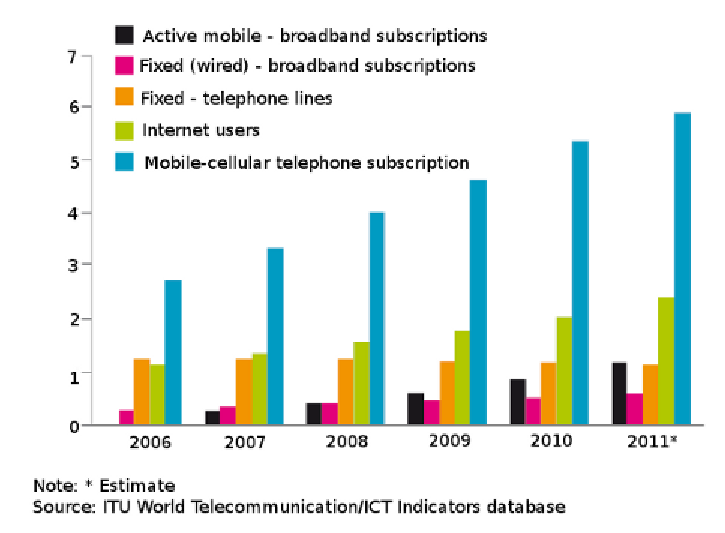
\includegraphics[scale=0.8]{./graph/mobuser1}
\caption{ICT lietotāju statistika laikā periodā 2006 - 2011 \cite{ict}}
\label{fig:mobilStat}
\end{figure}

Ekspromta tīklu plašais pielietojuma spektrs veicina gan šo tīklu ieviešanas pieaugošo intensitāti, gan arī nodrošina inovatīvo tehnoloģisko risinājumu pieaugumu. To, savukārt pastiprina aizvien pieaugošais lietojumprogrammu klāsts kuram sensoru tīkli ir paredzēti, sākot ar maza mēroga statiskiem tīkliem un līdz liela mēroga augsti mobiliem tīkliem. Pēdējā laikā ekspromta tīkli guva plašu interesi, un daudzi pētnieki saskata aiz vien pieaugošu potenciālu ekspromt tipa tīklu attīstībā. To pašreizējā attīstības stadija ir vēl tālu no tīkliem ar infrastruktūru. Un panākt Ad Hoc tīklā ātru, stabilu un uzticamu datu pārraidi ir grūts un ilgs process.
Taču, neraugoties uz to - jau šodien ar ekspromta tīklu palīdzību tiek izveidoti tīkli, kas ir paredzēti kādam vienam noteiktam mērķim, piemēram - tie tiek uzstādīti tādās vietās, kur infrastruktūras izveide nav iespējama \cite{self_manag}. Nākotnē, kad mobilo ekspromta tīklu pielietošana būs iespējama atbilstoši to pilnvērtīgam potenciālam, tiks nodrošināti tādi pakalpojuma veidi kas pieprasa stabilu savienojumu ar augstu \ac{QoS}, kā e-komercijas lietojumprogrammām, reāllaika video konferences, mobila režģa skaitļošanu (mobile grid computing), transportlīdzekļu sensora tīkls (\acs{VANET}) un daudzi citi.


%3. izvēlētās pētniecības metodes un objektus
\acf{QoS} prasības ir izstrādātas informācijas iegūšanai par lietotāja rīcībā esošajiem tehniskajiem resursiem, piemēram, datu apstrādes jaudas resursiem, datu uzglabāšanas resursiem un līdzīgi. Šādu prasību izstrādes nepieciešamību pamato ar plašo iekārtu daudzveidību un nepieciešamību nodrošināt to savstarpēju saderību un sadarbību. Kā rezultātā ir izstrādāti dažādu līmeņu QoS parametri un to izmantošanas kritēriji. Šie kritēriji var tikt tendēti uz jaudas parametru uzraudzību, attēlu rezolūcijas sinhronizācijas īpatnībām, dažādu platformu saderību, jeb pielagot citu parametru pielīdzināšanai kas būtiski ietekmē gan pārsūtāmo datu apjomu, gan, līdz ar to, arī kopējo QoS līmeni. Šī darba mērķis ir noteikt nepieciešamo BER līmeni kvalitatīvai datu pārraidei bezvadu sensor tīklos (WSN). Izmantojot diskrēto notiku datorsimulāciju un balstoties uz eksperimenta rezultātiem noteikt mobilitātes ietekmi uz QoS. Ņemot vērā laika ierobežojumu atvēlētu šī darba izstrādāšanai, pētīšanas apgabals tiks ierobežots sekojoši: a) tiks apskatīti plaši pielietojamo mobilitātes modeļu un komutācijas protokolu aspekti, b) tiks izvērtēta datu pārraides ātruma un maksimālo starpmezglu pārvietošanās ātrumu \gls{v_max} ietekme uz BER  un c) apskatīta dažādu protokolu veiktspēja mobilitātes apstākļos.
%4. un definē darba mērķus un uzdevumus,
Lai sasniegtu uzstādīto mērķi un skaitliskā viedā izteiktu mobilitātes ietekmi uz servisa kvalitāti (\acs{QoS}), šai darbā tiks veikts analītisks apskats par mobilajiem sensoru tīkliem un vēlāk darba gaitā tiks izstrādāta datorsimulācija \ac{NS-2} vidē. Lai sasniegtu mērķi ir nepieciešams:
\begin{enumerate}[label=\arabic*)]
\item Izpētīt mobilitātes ietekmi bezvadu sensoru tīklos (\acs{WSN}) un to ietekmi uz bitu kļūdu intensitāti (\acs{BER}).
\item Izpētīt mobilitātes ietekmi uz maršruta garuma daudzposmu maršrutā.
\item Balstoties uz eksperimentāli iegūtajiem rezultātiem (NS-2 simulācijas) izvērtēt analītiski iegūtos datus.
\end{enumerate}


\section{Literatūras apskats}\label{sec:lit}
Pēdējā laikā bezvadu sensoru tīkli (\acs{WSN}) piesaista lielu pasaules pētnieku interesi un tiek uzskatīti par potenciālu risinājumu visuresošai piekļuvei Internet tīklam \cite{perkinsBook,toh}. Šo vīziju īstenošana galvenokārt ir atkarīga no iespējas nodrošināt atbilstošu \acs{QoS} līmeni sensoru tīklos un tīkla mezglu mobilitāti. Nākamās paaudzes ekspromta tīkla (\acs{Ad Hoc}) mezgli būs mobili, piemēram, novietoti transportlīdzeklī \cite{dsdv_mobPc}. Izveidot un uzturēt daudzposmu savienojumu ir sarežģīts uzdevums nemitīgi mainošas topoloģijas apstākļos: daudzposmu maršrutā katra mezgla pozīcija nemitīgi mainās laikā un telpā. Tas rada nepieciešamību pārraudzīt visu mezglu novietošanu arī pēc maršruta izveidošanas, lai gadījumā, ja viens vai vairāki megli tiek izslēgti no aprites, tad vēl joprojām būtu iespējams uzturēt savienojumu starp gala punktiem \cite{park, lim, son}. R. Rao savā darbā \cite{rao} raksta, ka iepriekš projektēts mobilitātes modelis atstāj būtisku ietekmi uz eksperimenta rezultātiem.

2000. gadā P. Gupta un P.R. Kumar piedāvāja un pamatoja transportēšanas kapacitātes koncepciju \cite{gupta}. Koncepcija ņem vērā tīklā pārraidīto informācijas daudzumu un attālumu kādā šī informācija tiek pārraidīta. Šie parametri palīdz noteikt maksimāli ilgtspējīgu datu plūsmu daudzposmu ekspromta bezvadu tīklā. Tas nozīmē, ka teorētiski mobilitāte var paaugstināt tīkla datu pārraides kapacitāti (kā aprakstījis M.Grossglauser un D.Tse \cite{grossglauser}), bet praksē ekspromta tīkla (\acs{Ad Hoc}) tīkla veiktspēja samazinās mobilitātes dēļ \cite{perkins_hughes}. M.J.Neely un E.Modiano, lai sniegtu labāku priekšstatu par mobilitātes ietekmi pētāmais tīkls tiks apskatīts sadalīts šūnās, \seename \cite{neely1}. Tīkls ir vienības kvadrāts \footnote{kvadrāts Dekarta koordinātu sistēmā ar koordinātām (0, 0), (1, 0), (0, 1), un (1, 1)} kurā izvietoti mobilie mezgli. Šai gadījumā tīkls ir sadalīts šūnās, kas ir vienādas pēc izmēra un nepārklājas savā starpā, mezgli var izveidot savienojumu ja atrodas vienā un tajā pašā šūnā. Lai izvairītos no savstarpējiem mezglu traucējumiem (kā mezglu savstarpējie traucējumi  (\acs{INI})) tiek izmantotas četras dažādas frekvences (\seename ~\figurename .1, \cite{neely1}). Šis modelis balstīts uz kompromisu starp tīkla kapacitāti un pakešu aizkavi rindā. S.Toumpis savā darbā pēta maksimālo pārraides ātrumu un pārraides aizkaves augšējo robežu mobilajos mezglos sensora tīklā, ņemot vērā signāla rimšanas efektu \cite{toumpis}.

Jaunu paņēmienu ierosināja G.Ferrari un O.K.Tongus \cite{tonferBOOK}. Viņu ierosinātais paņēmiens atšķirās no \cite{neely1} aprakstītā un atšķirās ar to, ka statiski mezgli novietoti režģa četrstūros. Darbā tika izvērtēta tīkla veiktspējas izmaiņu atkarība no fiziskā slāņa īpašībām, kā arī analizēts vides piekļuves vadības (\acs{MAC}) protokols. Kombinējot rezervēšanas komutācijas (\acs{RBS}) metodi \cite{ferrari17} kā arī apskatot bez-rezervēšanas (\acs{NRBS}) metodi \cite{tonguz18}. Vēlāk savos darbos G.Ferrari un O.K.Tongus pēta mezglu mobilitātes ietekmi uz BER līmeni izmantojot to pašu mezglu izvietojumu \cite{tonferBOOK}.

Pārsvarā zinātniski raksti, kas ir publicēti par tēmu „Mobilie ekspromta tīkli”, savu pētījumu eksperimentālajā daļā izmanto IEEE 802.11 protokolu. IEEE 802.11 protokolā datu pārraidei tiek izmantots Wi-Fi vai Bluetooth interfeiss. Nesen tika izveidots jauns iterfeisa standarts - IEEE 802.15.4/ZigBee, kas vēl nav tik "populārs" kā IEEE 802.11.

\section{Tēmas aktualitātes pamatojums}
Kā jau iepriekš apskatīts, tad ekspromta tīklu pielietojums ikdienā kļūst aizvien plašāk izplatīts un ieņem aizvien būtiskāku lomu ikdienas vajadzību nodrošināšanā. Kā vienu no šāda mērķa sasniegšanas risinājumiem var uzskatīt vienu no jaunākajiem izstrādātajiem un IEEE apstiprinātajiem standartiem - 802.15.4/ZigBee. Šis protokols ir izstrādāts ar mērķi uzlabot un nodrošināt sensoru un kontroles pielietojamības iespējas mobilajos tīklos. Standarts paredz dažāda veida tīkla pašatjaunošanās iespējas. Tas, savukārt, nodrošina efektīvākus tīklu savstarpējās saslēgšanas risinājumus ar samazinātu enerģijas jaudu, kas savukārt palielina mobilo iekārtu mobilitāti un pagarina to darbības laiku.

Zinātniskajos institūtos visā pasaulē aiz vien lielāka uzmanība tiek pievērsta dzīves kvalitātes uzlabošanai, kas savukārt rada nepieciešamību organizēti grupēt un savstarpēji savienot plašu klāstu ekspromta tīklu. Kā piemēru var minēt Oslo inovāciju centra izstrādes stadijā esošo veselības aprūpes komplekso risinājumu - Dignio \cite{dingio}.
Dignio projekts paredz ražošanā ieviest kompleksu iekārtu, kuras uzdevums ir nodrošināt savienojumu ar plašu klāstu mobilo iekārtu risinājumiem, kā WLAN, WPAN, ZigBee, NFC un daudzi citi. Šādi risinājumi ne tikai būtiski veicina mobilā interneta piekļuves iespējas, taču vienlaicīgi nodrošina augsto tehnoloģiju un risinājumu ieviešanu ikdienas dzīvē, nodrošinot lietotājiem ne tikai divpusēju savienojumu ar uzraudzības centrāli, taču arī savienojumu ar vairumu ikdienā lietojamo bezvadu iekārtu. Šādu risinājumu izstrāde ir komplicēts darbs un prasa lielus resursu ieguldījumus zinātniskajā darbā.

Lai attiecīgajos risinājumos nodrošinātu augsta līmeņa iekārtu komunikāciju kvalitāti ir būtiski izvērtēt nepieciešamību nodrošināt lietotājam vienu no būtiskākajām prasībām - mobilitāti. Kas savukārt rada palielinātas prasības QoS nodrošināšanai jo pieaugot lietotāju mobilitātei tīklā var parādīties stohastiski raksturlielumi kas var būtiski ietekmēt QoS. Tādējādi šī maģistra darba tēmas aktualitāti var skaidrot ar nepieciešamību nodrošināt lietotājiem mobilitātes iespējas neatkarīgi no to prasībām.

\section{Pētāma tīkla parametri }\label{sec:petPar}
Mobilais sensoru tīkls tiek pieņemts ar sekojošiem parametriem:
\begin{enumerate}
	\item Datu pārraidei tiek izmantota $f_{c} = 915$ [MHz] frekvence.
 	\item Tīklam ir kvadrāta forma ar laukumu $S = 1500\times300$ un $500\times300$, [$m^{2}$]. Tīkla laukums ir konstants un nemainīgs simulācijas laikā.
  	\item Tīkla laukumā $S$ viendabīgi izkliedēti $N$ mobilie mezgli. Reālajā dzīvē tas varētu izpausties kā fakultātes vai lidostas ēka ar laukumu $S$, kurā pārvietojas cilvēki ar portatīviem datoriem vai/un mobiliem telefoniem. Cilvēki pārvietojas ēkā neaizejot ārpus tā laukuma, tajā pašā laikā cilvēku blīvums ēkā ir mainīgs $\rho_{s} = \frac{N}{S}$.  Mezglu skaits ir konstants lielums un $N = 51$ mezgls.
  	\item Katra mezgla pārraides jauda ir konstants lielums \gls{p_t} $= 1$ [mW] un tā minimālā uztveres jauda \gls{p_imin} $= - 94$ [dBm] arī konstants lielums.
  	\item Trafika ģenerēšanai tiek izmantots konstants bitu ātrums (\acs{CBR}) ar paketes garumu \gls{L} $= 512$ [b/pck] un datu pārsūtīšanas ātrums \gls{r_b} $= 2$ [Mbit/s]. CBR tiek izvēlēts, lai izslēgtu varbūtību, kā trafika variācija var ietiekmēt eksperementu rezultātus, līdz ar to labākais variants ir izvēlēties konstants trafiks. 
  	\item Starpmezglu interference. No vienādojuma (\ref{eq:ini}) izriet - lai samazinātu starpmezglu interferences līmeni ir nepieciešams lai $\lambda L/R_{b}$ būtu pēc iespējas mazs lielums (\seename~\cite{qoS_static}). Tiek uzskatīts, ka avota ražo informāciju  paketes. Katrs mezgls izveido paketes konstantā garumā pēc Puassona sadalījuma ar \gls{lambda} = 4 [pck/s].
  	\item Kanāla modulācija ir  binārā fāzes manipulācija (\acs{BPSK}).
  	\item Maršruta izveidošanas stadija netiek apskatīta un netiek ņemta vēra simulācijas rezultātu analīzē. Kā minēts \ref{sec:prot} nodaļā maršruta izveidošana ir viens no svarīgiem un sarežģītiem procesiem sensoru tīklā \cite{perkinsBook}. Lai sasniegtu šī darba uzstādīto mērķi (datu apmaiņas procesa pētīšana) tīkls tiks pētīts pēc sākotnēja maršrutu izveidošanas procesa.
  	\item Izmantots gadījuma maršrutpunktu mobilitātes modelis (\acs{RWMM}).
  	\item Starpmezgls ziņojumu nepārraida tālāk kamēr nav saņēmis visu ziņojumu.
  	\item Tiek pieņemts, ka komunikāciju kanāls ir ideāls: kaimiņ-mezgls uz $r_{link}$ distances ir nekavējoties pieejams.
	\item Enerģijas patēriņš netiks ņemts vērā darba gaitā.
\end{enumerate}

\section{Darba pārskats}
%5. sniedz nelielu ieskatu katrā no darba nodaļām numeroloģiskā secībā.
Šis darbs ir organizēts pēc sekojoša principa: Nodaļā \ref{sec:infra} apskatīti ekspromta tīklu veidi. Nodaļā \ref{sec:tris} ir apkopoti Ad hoc tīklu teorētiskie aspekti, kā tīkla formas matemātiskie interpretācijas veidi, BER aprēķināšanas veidi, mezglu ātrums un komutācijas veidi: Bez-rezervēšanas (\acs{NRBS}) un rezervēšanas-bāzētas (\acs{RBS}). Nodaļā \ref{sec:mobilityModels} ir apskatīti trīs visplašāk pielietojamie mobilitātes modeļi mobilo Ad hoc tīklu simulācijas: \acf{RWMM},\acf{RDMM} un \acf{OMM}. Kā arī \acs{RWMM} modelim ir aprakstīta daudzposmu maršruta garuma izmaiņa mobilitātes ietekmē. Nodaļā \ref{sec:prot} ir sniegts neliels ekspromta tīklu maršrutēšanas protokolu apskats tādiem protokoliem kā: \acf{AODV}, \acf{DSR} un \acf{OLSR}, kā arī piedāvāts jauns maršrutēšanas algoritms SP-BER.  Daži no šiem protokoliem ir vēlāk izmantoti NS-2 simulāciju scenārijos. Nodaļā \ref{sec:prakt} aprakstīti NS-2 simulācijas scenāriji un to rezultāti. Nobeiguma nodaļā \ref{sec:secin} ir izklāstīti secinājumi.
\chapter{Bezvadu Ad Hoc tīkli}\label{sec:infra}
Bezvadu tīklus var sadalīt divās pamatgrupās, tīkli ar iepriekšnoteiktu infrastruktūru un ekspromta tīkli. Tīklu ar iepriekšnoteikto infrastruktūru klasiskais piemērs ir mobilo sakaru tīkls un bezvadu lokālais tīkls (\acs{WLAN}).  Mobilo sakaru tīkla operators izvieto bāzes stacijas tā, lai nodrošinātu bezvadu savienojumu noteiktā diapazonā. Katrai no tīkla bāzes stacijām ir fiksēts ātrgaitas savienojums ar pamattīklu. Datu pārraide bezvadu vidē notiek vienā posmā starp mobilo mezglu un tuvāko bāzes staciju. Bezvadu ekspromta tīkls (\acs{Ad Hoc}) ir decentralizēts bezvadu tīkls \cite{perkinsBook}. Šādu nosaukumu ekspromta tīkls (\acs{Ad Hoc}) ir ieguvis jo tam nav iepriekš noteikta infrastruktūra, no latīņu valodas ''Ad Hoc'' tulkojams kā ''šim nolūkam''.  Ekspromta tīkls pilnībā izslēdz vadu savienojumu no tīkla infrastruktūras. Ekspromta tīkli pielietojami vietās kur tīkla uzbūve ir apgrūtināta vai neiespējama. Dotajā brīdī sensoru tīkli tiek plaši pielietoti militārās operācijās un pētnieciskos projektos kuriem tīkls nepieciešams grūti pieejamos rajonos (piemēram: kalnos, mežos, okeāna dziļumos, u.c.). Kā arī, ekspromta tīklus pielieto iekštelpās, piemēram, konferencēs savienojot vienotā tīklā vairākus klēpjdatorus. Ekspromt tīklā katrs tīklā esošais elements (turpmāk tekstā ''mezgls'') tiek uzskatīts par potenciālo pārraides posmu. Mezgli apvienoti tīklos lai nepieciešamības gadījumā nodrošinātu datu pārraidi. Mezgli varbūt datu avots, saņēmējs vai arī tie var darboties kā retranslējošs mezgls. Ekspromta tīklā mezgli var būt statiski,  mobili vai abi vienreiz. Ad Hoc tīklus var iedalīt sekojošos veidos:
\begin{enumerate}[label=\arabic*)]
    \item \acf{WSN} sastāv no teritoriāli izkliedētiem autonomiem sensoriem kuri novēro fiziskas vai apkārtējas vides izmaiņas, piemēram, temperatūras izmaiņas, vibrācijas, gaisa spiedienu vai piesārņojuma līmeni. Tīklā esošie mezgli izveido savienojumu lai pārraidītu iegūtos datus uz attālinātu pētniecisko centru (\figurename. ~\ref{fig:wsn}). WSN tīkla topoloģija variē no parastas zvaigznes topoloģijas līdz daudzposmu bezvadu režģtīklam (\acs{WMN}) ar tūkstošiem mezglu.
    \item Mobilais ekspromta tīkls (\acs{MANET}) vai Mobilais Ad Hoc tīkls, ir paškonfigurējošs decentralizēts tīkls, kas sastāv no mobilām ierīcēm savienotām savstarpēji ar bezvadu saitēm. Mobilajā ekspromte tīklā (\acs{MANET}) katrā ierīce spēj brīvi pravietoties jebkurā virzienā un nemitīgi mainīt savienojumu partnerus.
    \item Integrēts heterogēnu bezvadu tīkls (\acs{IHWN}) apvieno vienotā tīklā: satelīttīklu, GSM/3G, WiMAX, WPAN, MANET un LAN; aprakstīts IEEE 802.21 standartā.
\end{enumerate}
\begin{figure}[!htb]
\begin{minipage}[t]{0.5\linewidth}
\centering
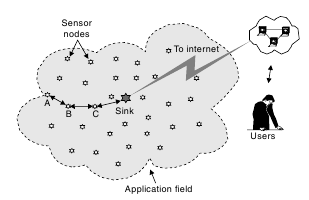
\includegraphics[scale=0.7]{./graph/wsn}
\caption{Bezvadu sensoru tīkls} \label{fig:wsn}
\end{minipage}%
\begin{minipage}[t]{0.5\linewidth}
\centering
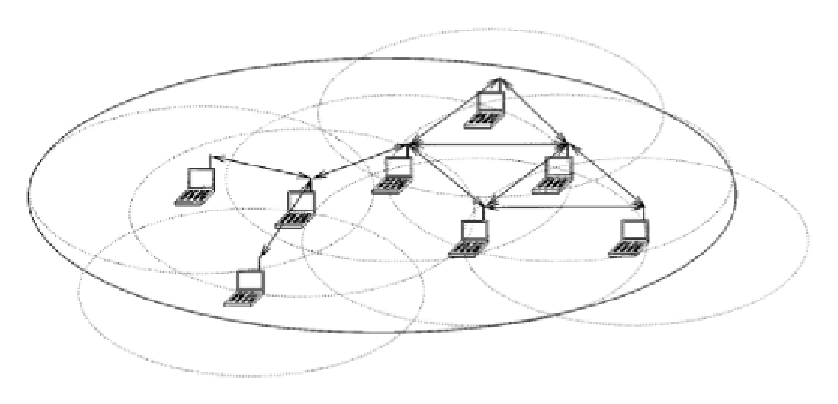
\includegraphics[scale=0.6]{./graph/adhoc}
\caption{Ekspromta tīkls} \label{fig:manet}
\end{minipage}
\end{figure}

\section{WSN un MANET salīdzinājums}
Bieži vien ir grūti noteikt precīzu robežu starp MANET un WSN tīkliem, jo abām topoloģijām ir kopīgas iezīmes un atšķirības ir novērojamas tikai niansēs. Taču šīs nianses izpaužas kā ļoti  svarīgi parametri maršrutēšanas protokolu dizainā.

\subsubsection{Līdzības}
MANET tīkla raksturīpašības ir sekojošas: relatīvi liels mezglu skaits, topoloģija nemitīgi un ātri mainās (dinamiskā topoloģija) un maršrutēšanas protokola pamatuzdevums ir nodrošināt efektīvu datu pārraidi dinamiskos topoloģijas apstākļos. Savukārt, WSN raksturo: ļoti mazas ierīces ar ārkārtīgi ierobežotiem resursiem, koncentrēta mezglu izvietošana, un maršrutēšanas protokola centrālais aspekts ir dati un energoresursu patēriņš. WSN un MANET ir līdzīgi sekojošos aspektos:\\
\small\textbf{\textit{Ad Hoc režīms.}} Nav nepieciešamības iepriekš definēt izmantojamo infrastruktūru vai bāzes staciju (BS). Mezgli savstarpēji sazinās caur vairākām bezvadu saitēm. Katrs tīkla mezgls spēj būt arī avots, galamērķis vai retranslēt paketes.  \\
\small\textbf{\textit{Resursu ierobežojumi.}} Abu tīklu mezgliem ir ierobežoti raidītāja jaudas resursi. Parasti MANET ierīces ir pārnēsājamas ierīces ar zemu raidītāju kapacitāti, piemēram, klēpjdatori, mobilie telefoni, PDA utt.  Sensoriem pieejamie jaudas resursi ir vēl zemāki. \\
\small\textbf{\textit{Enerģijas avotu ierobežojumi.}} Abiem visu mezglu darbība tiek nodrošināta ar mazjaudas akumulatoriem vai baterijām. Viens no svarīgākjiem sistēmas kritērijam ir enerģijas patēriņa samazi- nāšana. Lai ievērojami uzlabot sistēmas veiktspēju ir nepieciešami algoritmi, kas pārrauga enerģijas patēriņu.\\
\small\textbf{\textit{Bezvadu komunikācija.}} MANET un WSN ir izveidoti uz bezvadu komunikācijas kanāla bāzēm.

\subsubsection{Atšķirības}
No pirmā skatiena var rasties iespaids, ka WMN un MANET ir ļoti līdzīgi, taču starp abiem tīkla veidiem ir būtiskas atšķirības.\\
\small\textbf{\textit{Mezglu identificēšana.}} MANET tīklā mezgliem vienmēr ir vispārēji unikāls identifikators (\acs{GUID}), piemēram, MAC adrese vai IP adrese. Tas ir pamat adresēšanas princips visiem MANET maršrutēšanas protokoliem. WSN tīklā GUID tiek pielietots pēc nepieciešamības (ar AODV vai OLSR protokoliem) un iespējām.\\
\small\textbf{\textit{Resursi.}} Abiem - MANET un WSN tīkliem ir ierobežoti resursi, bet kritiskais līmenis katram ir savs. MANET mezglu resursi ir daudzkārt augstāki nekā WSN. MANET tīkls pārsvarā sastāv no pārnēsājamām ierīcēm, kuru procesora kapacitāte sasniedz simtus MHz; iebūvētās atmiņas tilpums ir no dažiem megabaitiem līdz gigabaitiem, to var palielināt ar atmiņas kartēm; akumulatoru kapacitāte nodrošina ierīces vairāku stundu darbību. Savukārt, WSN sastāv no ierīcēm ar ārkārtīgi ierobežotiem resursiem. Piemēram, Berkeley MICA2 sensors ir aprīkots ar 8-bitu ATmegall128 procesoru, iebūvētu 128K RAM, 4K EEPROM un 512K atmiņas karti \cite{Proc13}.\\
\small\textbf{\textit{Komunikācijas paradigma.}} MANET tīklā visi mezgli ir vienranga (peer-to-peer). Nevienam mezglam nav prioritātes un datu pārraidi var iniciēt ikviens tīkla mezgls. Apraide (broadcast) izmantota tikai maršruta izveidošanas procesā (handshake apmaiņai), savukārt ziņojumu pārsūtīšanai izmanto GUIDS adresi un ziņojumi adresēti vienam noteiktam galamērķim. WSN tīkla galveno lomu aizņem satekne (sink), tā ir vienīgā vārteja (gateway) starp tīklu un galalietotāju (\figurename. ~\ref{fig:wsn}). Satekne vienmēr iniciē datu pārraidi tīklā. Mezglu savstarpēja komunikācija ir reta parādība bezvadu sensoru tīklā. Savukārt, apraide un multiraide (multicast) ir ļoti bieži sastopama WSN tīklos, to ietekmi vienmēr jāņem vērā.\\
\small\textbf{\textit{Blīvums.}} Mezglu blīvums $\rho$ tiek definēts kā vidējais kaimiņ-mezglu skaits uz vienu mezglu tīklā \cite{NSsurvey}. Izmantojot disku grafu komunikācijas modeli (Unit Disk Communication Model) to aprēķinā pēc formulas \cite{perkinsBook}
\begin{equation}
\rho=\frac{(N\pi r_{link}^2)}{A} ,
\label{eq:blivums}
\end{equation}
kur $N$ ir kopējais sensoru skaits tīklā, A ir tīkla laukums un $r_{link}$ ir mezgla radio pārraides diapazons. MANET tīklos mezgli ir reti izkliedēti tīkla laukumā, turpretim WSN mezglu izvietojums ir biezs. Dažādu blīvumu dēļ tiek izmantoti dažādi paņēmieni robustuma novēršanai. Piemēram, MANET protokolā datu posms nodrošina lēkumu pārraidi un šī savienojuma izturība ir ļoti svarīga. Maršrutēšanas protokolu dizainā pievērš lielu uzmanību savienojuma izveidošanai un tā ilgstošai pastāvēšanai. WSN tīklos datu pārraide notiek bez apliecinājumu (acknowledgment) mehānisma pielietošanas, jo vienaposmā (one-hop) savienojums var būt ļoti nedrošs. No iepriekš minētā var secināt, ka pārraides kanāla noturība ir ļoti svarīgs aspekts \cite{20}.\\
\small\textbf{\textit{Bezvadu multiraides priekšrocība.}} WSN tīkla mezgls multiraides režīmā spēj vienlaicīgi raidīt datus $r_{link}$ diapazonā esošajiem kaimiņiem. Līdz mezgliem, kas atrodas ārpus šī diapazona, ziņojums nonāks kā troksnis. Savukārt, MANET tīklā pārraide notiek uz vienu noteiktu adresi.  \\
\small\textbf{\textit{Dizaina kritēriji.}} MANET tīklu galvenie izveidošanas un vērtēšanās kritēriji ir servisa kvalitāte (\acs{QoS}) un kanāla caurlaidspēja. Enerģijas patēriņš tiek atvirzīts otrajā plānā, jo ierīces akumulators var tikt nekavējoties uzlādēts vai aizvietots. WSN tīkls sastāv no liela neaprūpēta ierīču skaita, kurā akumulatora aizvietošana vai uzlādēšana ir sarežģīts proces. Līdz ar to maršrutēšanas galvenais mērķis ir pazemināt enerģijas patēriņu lai pagarinātu tīkla darbības laiku.\\
\small\textbf{\textit{Protokolu dizains.}} MANET tīkla protokoli tiek izveidoti pēc slāņu koncepcijas, kas savukārt ir iemantota no vadu tīkliem. Turpretī, WSN tīkls ir izveidots uz iegultās sistēmas (embedded system) bāzes un šai gadījumā ''visi-vienā'' (all-in-one) dizains ir piemērotāks. \\

\section{WSN un WMN salīdzinājums}
Bezvadu režģtīkls (WMN) sastāv no mezgliem kas caur bezvadu savienojumu retranslē citu mezglu paketes (\seename ~\figurename.~\ref{fig:wmn}, ar punktēto līniju apzīmēts bezvadu savienojums).
\begin{figure}[!htb]
\centering
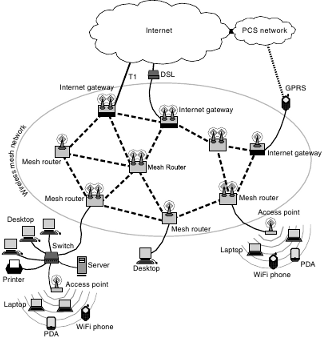
\includegraphics[scale=1]{./graph/wmn}
\caption{Bezvadu režģtīkls \cite{perkinsBook}}
\label{fig:wmn}
\end{figure}

 WMN tīklu pamatuzdevums ir retranslēt paketes  līdz režģtīkla globālā tīmekļa vārtejām (\figurename.~\ref{fig:wmn} ''Internet gateway''). Parasti režģtīkla mezglam ir raksturīgi sekojoši parametri: mezgli stacionāri, vai arī tiem piemīt minimāla mobilitāte; mezgli ir izvietoti uz māju jumtiem vai ielas apgaismojuma stabiem; atsevišķas vārtejas ar vadu ir savienotas ar pamattīklu. Mezgli aprīkoti ar vairākiem interfeisiem: Wi-Fi, Ethernet, Bluetooth un citi.

Kā pāradīts \figurename.~\ref{fig:wmn} WMN perfekti der pilsēttīkla (\acs{MAN}) izveidošanai. WMN spēj nodrošināt augstāku datu pārsūtīšanas ātrumu nekā mobilo telefonu tīkls, līdz ar to var nodrošināt kvalitatīvu IP balss pārraidi (VoIP) un citus multimediju servisus.
Pēc savas koncepcijas WMN it līdzīgs MANET, tas ir tādā ziņā, ka mobilās stacijas savā starpā komunicē izmantojot daudzposmu pārraidi. MANET un WMN ir būtiskas atšķirības:
\begin{itemize}
\item Režģtīkla mezgli pārsvarā ir stacionāri un tas ietekmē protokolu dizainu, savukārt MANET mezgli ir mobili.
\item WMN tīkla caurlaidspēja ir svarīgs faktors, jo WMN tīklā spēj operēt simti vai pat tūkstoši mezglu. Arī tīkla mērogojamība ir svarīgs jautājums WMN tīkla dizainā.
\item Enerģijas patēriņš nav tik svarīgs, jo pamatā režģtīkla mezgli ir tieši savienoti ar elektroenerģijas tīklu. Tas ļauj izmantot jaudīgāku aparatūru režģtīkla mezgliem.
\end{itemize}

\section{Bezvadu interfeiss}
Ad hoc tīklos ir pielietojamas vides piekļuves vadības (\acs{MAC}) balstītas bezvadu tehnoloģijas, kas pārsvarā darbojas ISM frekvenču joslā (Industrial Scientific and Medical band). Radio kanāli, kas darbojas ISM frekvences joslā, saņem papildus interferenci no tīklā neiesaistītām ierīcēm kas darbojas ISM, piemēram, mikroviļņu krāsnis. Šajā sadaļā netiks apskatīti visi IEEE 802 ģimenes standarti, bet tikai tie ar kuriem aprīkots vairākums no PDA, portatīvajiem datoriem kā arī mobilie telefoni un kurus iespējams izmantot Ad Hoc tīklu izveidē.

\begin{table}[!ht]
    \begin{tabular}{|l|c|c|c|c|c|c|}
        \hline
~              &802.11a&802.11b&802.11g&802.11n&802.15.1&802.15.4\\ \hline
Frekvence,[GHz]&5      &2.4    &2.4    &2.4    &2.4,     &2.4\\
              ~&      ~&      ~&      ~&     ~ &5        &0.868,0.915\\
Tehnoloģijas   &OFMD   &DSSS   &OFMD   &OFDM   &FHSS     &DSSS\\
Pārraid.ātrums,[Mbit/s]&54     &11     &54     &250      &3  &20-250$^{1}$\\
Antenas jauda,[mW]&20-40&100   &20-50  &250    &1,2.5&1\\
Diapazons,[m]  &120     &140   &140    &250    &10       &75\\
Tips           &\multicolumn{4}{c|}{WLAN}&\multicolumn{2}{c|}{WPAN}\\
 Enerģ.pateriņš Tx [mA]&\multicolumn{4}{c|}{400+}&40     &30\\
      'standby' režīma [mA]  &\multicolumn{4}{c|}{20}&0.2        &3\\\hline
\multicolumn{7}{r}{ \footnotemark[1]\footnotesize{Kbit/s}}
    \end{tabular}
\caption{IEEE 802 standartu apkopojums}
\end{table}

\begin{figure}[!htb]
 \centering
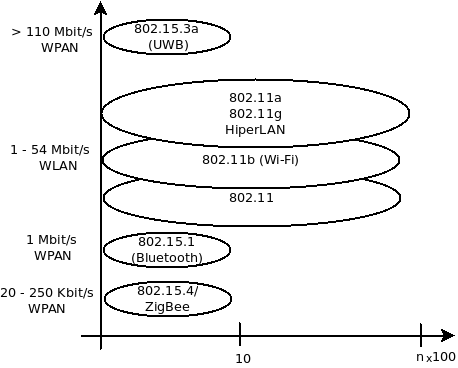
\includegraphics[scale=0.6]{./graph/wireless.png}
\caption{IEEE 802 bezvadu tehnoloģijas}
\end{figure}

% B. Mac Protocol - IEEE 802.11 Standard
% The distributed coordination function (DCF) of IEEE 802.11 [10] for wireless local area networks (WLANs) is used as the medium access control (MAC) protocol. The IEEE 802.11 DCF uses Request-to-send (RTS) and Clear-to-send (CTS) control packets for “unicast” data transmission to a neighboring node. The RTS/CTS exchange anticipates the data packet transmission and implements a form of virtual carrier sensing and channel reservation to reduce the impact of the well-known hidden terminal problem [11]. Data packet transmission is followed by an acknowledgment (ACK). All the packets are transmitted at maximum power. “Broadcast” data packets and RTS control packets are sent using physical carrier sensing. An un-slotted CSMA technique with collision avoidance (CSMA/CA) is used to transmit these packets. The considered node model has characteristics similar to those typical of the commercial radio interface in Lucent’s WaveLAN [12].



\subsection{IEEE 802.11}
Šobrīd visplašāk  pieejamais bezvadu datu pārraides interfeiss ir IEEE 802.11 ģimenes tehnoloģijas, kas pārsvarā darbojas 2.4 GHz frekvenču diapazonā izņemot IEEE 802.11a 5 GHz. Wi-Fi datu pārraides segums ir atkarīgs no  ierīces antenas jaudas un vides kurā signāls izplatās. Tīkla pārklājums variē no 50 līdz 100 metriem.

\subsubsection{IEEE 802.11a}
IEEE 802.11a izmanto ortogonālo frekvenčdales multipleksēšanas (\acs{OFDM}) tehnoloģiju un ir vienīgā bezvadu radio tehnoloģija kura darbojas 5 GHz frekvenču joslā.  IEEE 802.11a standarta datu pārraides ātrumi varbūt [6, 9, 12, 18, 24, 36, 48, 54] Mbit/s. Standartā rekomendējamais datu pārraides ātrums ir 24 Mbit/s, bet IEEE802.11a ierīču ražotāji palielina to līdz 54 Mbit/s (tas ir atļauts standartā). 54 Mbit/s ir maksimālais pārraides ātrums, bet reālistiskos apstākļos sasniedz 24 Mbit/s. Pēc CISCO publicētiem datiem pārraides jauda ir 40 mW pie [6 - 24] Mbit/s un 20 mW pie maksimāla datu pārraides ātruma 54 Mbit/s \cite{cisco}.

\subsubsection{IEEE 802.11b}
IEEE 802.11b izmanto tiešās secības spektra paplašināšanas (\acs{DSSS}) tehnoloģiju un darbojas 2.4GHz frekvenču joslā. Datu pārraides ātrums ir [1, 2, 5.5, 11] Mbit/s. Datu pārraides distance ir 90 m pie 1 Mbit/s un ap 30 m pie 11 Mbit/s. Ar maksimālo jaudu 100 mW pie visiem pārraides ātrumiem \cite{cisco}. No IEEE 802.11 ģimenes standartiem šis standarts ir viss biežāk pieejams mobilajās ierīcēs.

\subsubsection{IEEE 802.11g}
IEEE 802.11g tāpat ka IEEE 802.11a izmanto izmanto OFDM, un kā IEEE 802.11b darbojas 2.4GHz frekvenču joslā. Maksimālais datu pārraides ātrums ir 54 Mbit/s, savukārt reālistisks ir 22 Mbit/s. Tapat kā IEEE 802.11a standartā datu pārraides ātrums var būt [6, 9, 12, 18, 24, 36, 48, 54] Mbit/s un antenas pārraides jauda ir 50 mW pie [6 - 24] Mbit/s un 20 mW pie 54 Mbit/s \cite{cisco}.

\subsection{IEEE 802.15}
IEEE 802.15 standarts nosaka bezvadu personālā apgabala tīkla (\acs{WPAN}) standartus. Tas iekļauj informāciju par fiziskā (PHY) un \acs{MAC} slāņa specifikāciju bezvadu savienojumiem izveidošanai stacionārām, portatīvām un mobilām ierīcēm, kas darbojas PAN apgabalā.

\subsubsection{IEEE 802.15.1}
IEEE 802.15.1 standartā aprakstītā tehnoloģija ir plašāk pazīstama kā Bluetooth tehnoloģija. Bluetooth signāla modulācijai izmanto frekvences lēkāšanas (\acs{FHSS}) tehnoloģiju, kas arī darbojas 2.4 GHz frekvenču joslā. Šīs tehnoloģijas datu pārraides diapazons ir ierobežots līdz 10 metriem un datu pārraides ātrums ir 1 Mbit/s. Bluetooth antenas jaudas: Klase 1 ir 100 mW ar raidīšanas distanci $\approx$ 100m; Klase 2 ir 2.5 mW ar distanci $\approx$ 10 m; Klase 3 ir 1 mW ar distanci $\approx$ 5 m.

\subsubsection{IEEE 802.15.4/ZigBee}
IEEE 802.15.4/ZigBee tehnoloģija izmanto tiešās secības spektra paplašināšanas (\acs{DSSS}) tehnoloģiju un darbojas 2.4 GHz, 915 MHz un 868 MHz frekvenču joslās. Datu pārraides ātrums ir 250 Kbit/s pie 2.4 GHz, 40 Kbit/s pie 915 MHz un 20 Kbit/s pie 868 MHz. IEEE 802.15.4 MAC slānis ir nesēja jušanas un sadursmju nepieļaušanas daudzpiekļuves (\acs{CSMA/CA}) metodi, tapāt kā IEEE 802.11 ģimenes standarti. Datu pārraides diapazons ir no 10 līdz 75 metriem un antenas jauda ir 1 mW.
Šeit svarīgi atzīmēt ka ZigBee nav IEEE 802.15.4 standarts. IEEE 802.15.4 standarts ir zemo-ātrumu bezvadu personālā apgabala tīkls (\acs{LR-WPAN}), savukārt ZigBee ir specifikācija kurā PHY un MAC slāņos izmanto IEEE 802.15.4 standartu.
\begin{figure}
\centering
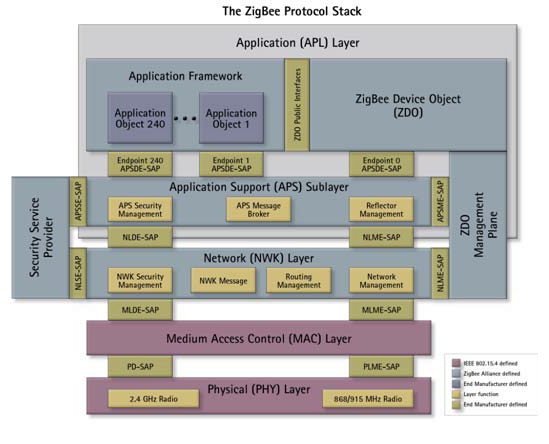
\includegraphics[scale=0.95]{./graph/zigBee.png}
\caption{IEEE 802.15.4/Zigbee \cite{libelium}}
\end{figure}

% \section{Tehnoloģijas izvēles pamatojums}
% WSN tīklu galvenas raksturīpašības ir: augsts mezglu blīvums, ierobežots enerģijas avots, Ad-Hoc režīms. No IEEE 802 standartu ģimenes IEEE 802.15.4/ZigBee standarts izpilda visas. Pirmkārt ZigBee nodrošina zemo enerģijas patēriņu ar to ka tam ir tikai divi darbības režīmi: 1)Pārraides/Uztverēs un 2)miega (Sleep). Atkarība no ierīces konfigurācijas (galvenokārt raidītajā jaudas)  baterijas darbības laiks variē no mēnešiem līdz pat gadiem. Otrkārt, ZigBee ierīces spēj darboties trijās ISM joslas: 2.4GHz un 868/915 MHz. Augstfrekvences josla ir vispasaules pieejama un zemāka josla Ziemeļamerikā, Eiropā, Austrālijā un Jaunzēlandē. Un treškārt ZigBee varbūt dažādas topoloģijas: zvaigžņtīkla, režģtīkla un  vienādranga arhitektūra.
% \begin{table}[!ht]
%     \begin{tabular}{|c|l|l|l|}
%         \hline
% Frek. josla,[MHz]& 868.3&902-928&2400-2483.5\\ \hline
% Kanālu sk.&1&10&16\\
% Joslas platums,[KHz]&600&2000&5000\\
% Pārraides ātrums,[Kbit/s]&20&40&250\\
% Symbol Rate[1/sec]&20&40&62.5\\
% Frek. stabilitāte&\multicolumn{3}{|c|}{40ppm}\\
%         \hline
%     \end{tabular}
% \caption{IEEE 802.15.4 standarta PHY slāņa parametri}
% \end{table}
\chapter{Ad Hoc tīkla teorētiskie aspekti}\label{sec:tris}

\section{Komunikācijas modeļi}
Tīklā notiekošie procesi var būt apskatīti kā fizikālie procesi vai arī kā protokolu norises darbība. Savā grāmatā Perkins piedāvā divus Protokolu un fizisku komunikācijas modeļus \cite{perkinsBook}. Protokola modelis (\textit{Protocol Model}) nosaka, ka mezgls $i$ veiksmīgi pārraida mezglam $j$, ja kaimiņ mezgls $X_{k}$ uzsākot pārraidi nepārraus savienojumu starp $X_{i}$ un $X_{j}$ mezgliem. Matemātiski to var izteikt sekojoši:
\begin{equation}
 \mid X_{k}-X_{j}\mid\geq(1+\Delta)\mid X_{i}-X_{j}\mid ,
\end{equation}
savienojums starp $X_{i}$ un $X_{j}$ mezgliem.
Fiziskais  modelis (\textit{Physical Model}) nosaka, ka mezgls $i$ veiksmīgi pārraida mezglam $j$, ja mezglā $j$ signāla un interferences attiecība (\acs{SIR}) ir
\begin{equation}
 SIR=\frac{\frac{P_{t}}{|X_{i} -X_{j}|^\alpha}}{N_{o}+\sum\limits_{k\neq i}\frac{P_{k}}{|X_{k}-X_{j}|^\alpha}}\geq\beta ,
\end{equation}
kur \gls{p_t} ir mezgla $i$ pārraides jauda, $\alpha$ ir pārraides trakta zudumu koeficients, $N_{o}$ ir trokšņa līmenis un $\beta$ ir minimālā nepieciešama signāla un interferences attiecība (\acs{SIR}) kas ir nepieciešams veiksmīgai datu pārraidei.  Gadījumā kad $\alpha >2$ un visi mezgli pārraida ar vienādu $P_{t}$, abu modeļu aprēķinu rezultātiem ir jābūt vienādiem \cite{perkinsBook}.


\section{Tīkla modeļi}
\subsection{Statiskais ekspromta tīkls}
Savā darbā P.Gupta un P.R.Kumar \cite{gupta} pēta statisko bezvadu tīklu caurlaidspēju. Tīkla modelis ir vienības sfēra kurā novietoti $n$ identiski mezgli. Skaitlis $n$ ir nemainīgs un mezgli izvietoti nejauši. Visi mezgli raida vienā kanālā un mezgli savstarpēji traucē izraisot interferenci. No avota līdz galamērķim paketes tiek pārraidītas pa daudzposmu maršrutu, izveidotie maršruti ir taisnas līnijas (iespējamais īsākais ceļš). Katrs mezgls var būt arī avots, galamērķis vai retranslējošs mezgls. Izmantojot Voronoi diagrammu ar sfēras virsmu $S^2$ (\seename ~\figurename.~\ref{fig:voronoi}), viņi pierādīja ka eksistē tāda Voronoi diagramma kas nodrošina:
\begin{itemize}
 \item Katra Voronoi šūna $V \in \nu_{n}$ iekļauj sevī disku ar laukumu $\frac{100\log{n}}{n}$ un
 $\rho(n)$ vienāds ar diska rādiusu ar laukumu $\frac{100\log{n}}{n}$ uz $S^2$ virsmas.\footnote{Šī diska laukums uz $S^2$ virsmas ir mazāk par $\pi \rho^2$}
\item Katra Voronoi sūna ir ietverta diskā ar rādiusu $2\rho(n)$
\end{itemize}

\begin{figure}[htb!]
\centering%

\includegraphics{./graph/voronoi}
\caption{$S^2$ virsmas Voronoi diagramma uz sfēras \cite{gupta}}
\label{fig:voronoi}
\end{figure}

Pārejot uz 2-dimensionālo plakni rādiuss būs $e(n) = c\sqrt{n\log(n)}$, ar konstanti $c$ lielāku par 0. Tīkla mezgli ir nejauši izvietoti līdz ar to visām Voronoi šūnām $V \in \nu_{n}$ ir iregulāra forma un katrā no šūnām ar $\zeta \geq 1-\frac{c}{n}$ varbūtību ir izvietots vismaz viens mezgls, kur $c$ lielums atbilst savienojuma prasībām \cite{gupta}. Izēveloties mezglu pārraides diapazonu $8e(n)$, tas ļauj nodrošināt komunikāciju ar kaimiņ-mezgliem kas atrodas $8e(n)$ attālumā. Divas šūnas izraisa savstarpējus traucējumus, ja viena no šūnām ir mezgla $(2+\Delta)8e(n)$ attālumā no jebkuras mezgla otras šūnas. $\Delta$ ir pozitīvs skaitlis, to pielieto modelējot situāciju, kad ir nepieciešamība nepiļaut blakus esošiem mezgliem pārraidīt vienlaicīgi vienā kanālā.

Izmantojot ''\textit{Protocol}'' un ''\textit{Physical}'' modeļus var pierādīt, ka statisko bezvadu ekspromta tīklu caurlaidspēja vienāda ar $\Theta({\frac{1}{\sqrt{n}}})$ gadījuma kad mezgli ir patvaļīgi novietoti tīkla laukumā. Un $\Theta(\frac{1}{\sqrt{n\log(n)}})$ ar nejauši izvietotiem mezgliem. Neņemot vērā to, kādā veidā ir izvietoti mezgli, caurlaidspēja samazinās pieaugot kopējam $n$ mezglu kaitam.


\subsection{Mobilais Ad Hoc tīkls ar viena-posma maršrutu}
Grossglauser un Tse \cite{grossglauser} pievādā izmantot viena-posma datu pārraides shēmu MANET. Šī shēma izmanto vienkāršo trakta izplatīšanas modeli, kurā datu avots izvēlas īsāko maršrutu (short-path) un rezervē to. Kaimiņmezgli tiek izvēlēti kā retranslējoši, ja tie ir tieši savienoti ar galamērķi (tikai viens posms). Tīkla modelis ir normalizēts vienības disks kura laukumā izvietoti $n$ mobilie mezgli. Lai atvieglotu analīzi, tiek pieņemts, ka informācijas apmaiņa notiek laika intervālos. Atrašanās vieta mezglā $i$ laika periodā $t$ apzīmēta ar $X_{i}(t)$. $\{X_{i}(\cdot)\}$ kas ir stacionārs un ergodisks process izkliedēts uz diska virsmas, kura mezgli kustas pēc neatkarīgi un viendabīgi izkliedētas (\acs{iid}) trajektorijas. Katrā no laika intervāliem, plānotājs izlemj kurš no mezgliem būs datu avots, retranslējošs mezgls vai galamērķis. Tādā veidā tiek panākts, ka pāris avots - galamērķis ir nemainīgs laika periodā.

Avotam $i$ ir ziņojums uz galamērķi $d(i)$ laika periodā $t$. Tā kā mezgliem $i$ un $d(i)$ savienojums ilgst vidēji $\frac{1}{n}$ laikā periodu, tad ziņojums būs piegādāts $d(i)$ $\frac{1}{n}$ vai $\frac{2}{n}$ maršrutā ar retranslējošo mezglu. Grossglauser un Tse pieņem ka katra pakete var būt pārsūtīta ne vairāk kā vienu reizi.

Saskaņā ar $Physical Model$ laika brīdī $t$ mezgls $j$ var saņemt informāciju no $i$ ar noteikto ātrumu $B$ [b/sec] , ja
\begin{equation}
SIR=\frac{P_{t}(t)g_{ij}(t)}{N_{0}+\frac{1}{M}\sum\limits_{k\neq
i}P_{k}(t)g_{ij}(t)}=\frac{P_{t}(t)g_{ij}(t)}{N_{0}+\frac{1}{M}I}\geq\beta,
\end{equation}
kur $P_{t}(t)$ ir mezgla $i$ pārraides jauda, $g_{ij}(t)$ - savienojuma garuma pieaugums no mezgla $i$ līdz $j$, $M$ - sistēmas apstrādes pieaugums un $I$ kopējā interference mezglā $j$. Savienojuma garuma pieaugums $g_{ij}(t)$ ir no attāluma atkarīga funkcija \cite{grossglauser},
\begin{equation}
 g_{ij}(t)=\frac{1}{|X_{i}(t)-X_{j}(t)|^\alpha}=\frac{1}{r_{ij}^\alpha(t)},
\end{equation}
kur $r_{ij}(t)$ ir attālums starp $i$ un $j$.

No iepriekš teiktā izriet, ka katrs no mezgliem nosūta datus divos etapos. Pirmajā etapā notiek pakešu pārraide no avota uz retranslācijas mezglu un otrajā no retranslācijas mezgla uz galamērķi. Abi posmi notiek paralēli, bet  2. etapam ir absolūta prioritāte visos ieplānotajos avots-galamērķis pāros. Tādēļ, ka mezglu trajektorija ir neatkarīga un viendabīgi izkliedēta un sistēma atrodas stabilā stāvoklī, ilgtermiņa caurlaidspēja starp jebkuriem diviem mezgliem ir vienāda ar varbūtību ka šie divi mezgli tiks izvēlēti kā iespējamie avots-galamērķis pāris. Saskaņā ar \cite{grossglauser} šī varbūtība ir vienāda ar $\Theta(\frac{1}{n})$. Nejauši izvēlētais avots-galamērķis pāris var tikt savienots tieši vai caur vienu retranslējošo mezglu. Tādējādi, pakalpojuma līmenis ir $\lambda_{j} = \Theta(\frac{1}{n})$ izmantojot retranslācijas mezglu vai tiešo savienojumu. No tā izriet, ka kopējā caurlaidspēja avots-galamērķis pārim $\lambda_{T}$ ir
\begin{equation}
 \lambda_{T}=\sum\limits_{j=1, j\neq i}^{n}\lambda_{j}=\sum\limits_{j=1, j\neq
i}^{n}\Theta
(\frac{1}{n})=\Theta\lgroup\frac{n-1}{n}\rgroup\xrightarrow{
n\rightarrow\infty} \Theta(1).
\end{equation}
Tātad šī shēma sasniedz $\Theta(1)$ caurlaidspēju avots-galamērķis pārī tad, kad $n$ mezglu skaits tiecas uz bezgalību. Tomēr tāda viena lēkuma pārraide izraisa lielu pakešu aizkavēšanos un attiecīgi ar $n$ pieaugumu tiecas uz bezgalību.

\subsection{Mobilais Ad Hoc tīkls ar daudzposmu maršrutu}\label{sec:moby}
O.Tonguz savā darba \cite{qoS_mobility} piedāvā jaunu veidu kā reprezentēt mobilā tīkla topoloģiju. Lai mazinātu malas efektu, tiek uzskatīts ka tīkla virsma ir apļa  forma. Šis pieņēmums palīdz vienkāršot aprēķinus, jo mezgliem kas izvietoti pie pašas tīkla robežas ir mazāks kaimiņ-mezglu skaits salīdzinājuma ar pārējiem mezgliem. Gadījumā, ja tīkla virsma ir apaļa virsma, tad visiem tīklā esošajiem mezgliem ir vienāds kaimiņu skaits  neatkarīgi no tā, vai tas atrodas uz tīkla malas vai centrā. Šeit ir svarīgi atzīmēt ka, dēļ šī pieņēmuma var rasties neliela atšķirība ar reālo sensoru tīklu.

\begin{figure}[ht!]
 \centering
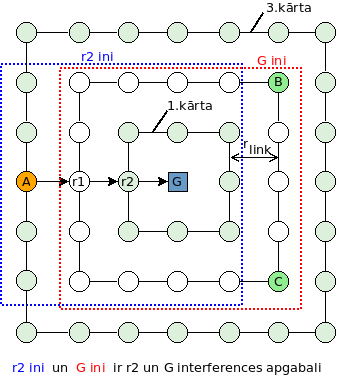
\includegraphics[scale=0.6]{./graph/tier.png}
\caption{Mobilo mezglu novietošana tīklā}
\label{fig:topo}
\end{figure}

Lai iegūtu ieskatu šajā problēmā, tiek pieņemts, ka tīkls ir taisnstūra režģis ar mezgliem izvietotiem to krustojumos un katram mezglam ir četri tuvākie kaimiņi (\seename~\figurename.~\ref{fig:topo}). Sakarā ar kvadrāta režģveida struktūru attālums līdz tuvākajam kaimiņam  ir fiksēts lielums \gls{r_link}  un maršruts līdz jebkuram mezglam ir vienāds ar vienāda garuma posmu virkni. Konstruējot kvadrāta režģi no $N$ mezgliem uz apļa virsmas ar laukumu $A$ ir viens un tas pats kā $N$ mazie kvadrāti ar laukumu $r_{link}^{2}$ ievietot lielā kvadrātā  ar laukumu $A$. No kā izriet ka $Nr_{link}^{2} = A$ un līdz ar to attālums starp diviem tuvākiem kaimiņiem var tikt izteikts sekojoši \cite{qoS_mobility}:
\begin{equation}
r_{link}=\sqrt{\frac{A}{N}}=\frac{1}{\sqrt{\rho_{s}}}
\label{eq:rlink}
\end{equation}
Kur \gls{rho} ir mezglu telpiskais blīvums. Tātad, kāda laika perioda $t$ avotam $n_{A}$ ir ziņojums uz galamērķi $n_{G}$ (att.~\ref{fig:topo}). Maršruts no $n_{A}$ līdz $n_{G}$ izmanto 2 retranslējošus mezglus ($r_{1}$, $r_{2}$) un tā kopējais garums ir 3$r_{link}$. Līdz ar to attālums starp avotu-galamērķi ir $i\times r_{link}$, $i$ ir kārtas numurs. Kā pāradīts att.~\ref{fig:topo} mezglam $n_{G}$ ir 7 kaimiņ-mezgli kas arī laikā brīdi $t$ var pārraidīt uz citiem mezgliem. Pieņemsim, ka divi kaimiņ-mezgli $k_{B}$ un $k_{C}$ arī raida. Tad $n_{G}$ SINR būs
\begin{equation}
SINR=\frac{Pt_{2}(t)r_{link}}{P_{trok}+P_{ini}},
\end{equation}
kur $Pt_{2}(t)r_{link}$ ir jauda saņemta no mezgla $r_{2}$, $P_{trok}$ ir kanāla trokšņu jauda un $P_{ini}$ ir interferējoša signāla jauda. Šai gadījumā $P_{ini}$ ir signālu summa saņemto no $k_{B}$ un $k_{C}$. Tad tad iepriekšējo formulu var pārrakstīt sekojoša veida:
\begin{equation}
SINR=\frac{P_{r_{G}}}{P_{trok}+P_{ini}}=\frac{Pr/P_{trok}}{1+(P_{r_{A}}+P_{r_{B}})/P_{trok}}.
\end{equation}


\section{Daudzposma maršruta garums}\label{sec:route}
Vienādranga bezvadu sensoru tīklos ar avots-galamērķis pāriem, gadījuma izvēlēto posmu skaits maršrutā ir gadījuma lielums un ir atšķirīgs katram maršrutam. Lai izvērtētu tīkla  veiktspēju  par maršruta garumu tiek pieņemts viduvējs maršruta garums. Tīkla virsma ir aplis un avots ir izvietots tīkla centrā (kā parādīts \figurename. ~\ref{fig:topo}). Ja galamērķis ir izvēlēts nejauši, tad minimālais posmu skaits līdz galamērķim būs intervālā no 1 līdz $2i_{n}$, kur $i_{n}$ ir  kārtas maksimālā pakāpe. Kas nozīme ka līdz pirmās kārtas kaimiņiem attālums ir viens posms un lai sasniegtu n-tas kārtas kaimiņus ir jāceļo $2i_{n}$ posmi. Posmu vidējo skaitu iegūst, izrēķinot posmu skaitu maršrutā no avota līdz katram iespējamam galamērķim un pēc tam aprēķinot vidējo vērtību. Pieņemot, ka katrs galamērķis ir vienlīdzīgi iespējams, vidējais posmu skaits maršrutā ir

\begin{equation}
\bar{n}_{h}=\frac{1}{N-1}\left[4 \sum^{i_{n}}_{i=1}i+4\sum^{i_{n}}_{i=1}2i+8\sum^{i_{n}}_{i=1}\sum^{i-1}_{j=1}(i+j)\right]
\label{eq:average}
\end{equation}

Kur pirmā summa atbilst posmu skaitam lai sasniegtu jebkuru no četriem centrētu mezglpunktiem visās tīkla $i$ kārtās; otra summa atbilst nepieciešamam posmu skaitam, lai sasniegtu jebkuru no četriem stūru mezglpunktiem visās tīkla $i$ kārtās; pēdējā -trešā divkārtīgā summēšana atbilst nepieciešamam posmu skaitam lai sasniegtu parējos mezglpunktus visās tīkla $i$ kārtās. Vienkāršojot (\ref{eq:average}) vienādojumu iegūs

\begin{equation}
\bar{n}_{h}=\frac{2}{N-1}\left (2i^3_{n}+3i^2_{n}+i_{n}\right )
\label{eq:sim_average}
\end{equation}
Tā kā $i$-tajā kārtā ir $8i$ mezgli, tad gadījumā, kad tīkla mezglu skaits ir pietiekami liels $i_{n}\simeq\frac{\sqrt{N}}{2}$. Tad (\ref{eq:sim_average}) formulā aizvietojot $i_{n}$ ar $\frac{\sqrt{N}}{2}$ iegūs\\
\begin{equation}
\bar{n}_{h}=\frac{(2+N)\sqrt{N}+3N}{2(N-1)}
\label{eq:aver_final}
\end{equation}
$\bar{n_{h}}$ var būt tikai vesels skaitlis, un (\ref{eq:aver_final}) rezultāts jānoapaļo uz augšu līdz tuvākajam veselam skaitlim.

Lai izveidotu daudzpusējo priekšstatu par pētāmā tīkla maršruta garumu ir nepieciešams aprēķināt $n^{max}_{h}$. Kā iepriekš jau bija minēts, tīkla virsma ir apļveidīga, tātad iespējamais garākais maršruts ir tad ja avots un galamērķis novietoti uz loka diametrāli pretējās pozīcijās. Šādā gadījumā visgarākais maršruts ir
\begin{equation}
n^{max}_{h}=\frac{2r_{A}}{r_{link}},
\end{equation}
kur $r_{A}$ ir virsmas rādiuss ($A=\pi r_{A}^2$). Aizvietojot $r_{link}$ ar (\ref{eq:rlink}) izteiksmi iegūst ka:
\begin{equation}
n^{max}_{h}=\lceil 2\sqrt{N/\pi}\rceil
\end{equation}
kur $\lceil\cdot\rceil$ ir noapaļošana līdz lielākajam veselam skaitlim.

Iegūtais $n_{max}$ ir neprecīzs lielums, jo daudzposmu maršruts var ''cilpot/riņķot'' ap taisno līniju novilktu starp avotu un galamērķi. Ņemot vēra faktu ka maršrutēšanas protokols ir "inteliģents" un ideālā gadījumā tiecas uz iespējami īsāko maršrutu, tad $n_{max}=\Theta\sqrt{N}$ neatkarīgi no tīkla virsmas formas \cite{cormen}.

\section{BER līmenis daudzposmu maršrutā}\label{sec:BER}
Daudzposmu maršruta katrā savienojuma uztvērēj-mezglā notiek datu reģenerācija un pārsūtīšana tālāk. Pieņemsim, ka ieviesušās kļūdas netiek izlabotas un kļūdas akumulējas visā maršruta garumā. Tad maršrutā $i$-tā posma bitu kļūdu intensitātes (\acs{BER}) līmenis starp diviem kaimiņ-mezgliem (\gls{ber_link}) ir atkarīgs no  signāla un trokšņa attiecības (\acs{SNR}) uztvērēj-mezglā ($SNR_{link}$) un radiokanāla raksturīpašībām. Savukārt, BER daudzposmu maršruta beigās būs \cite{qoS_static}:
\begin{equation}
BER_{route} = 1- \prod^{n-1}_{i=1}(1-BER_{link}^{(i)}),
\label{eq:BER_routeProd}
\end{equation}
kur n ir posmu skaits maršrutā. Lai nodrošinātu pieņemamu BER līmeni, maršruta beigas ir nepieciešams nodrošināt pēc iespējas zemāku BER katrā no posmiem,  $BER_{link} \ll 1$. Tad $BER_{route}$ tuvināta vērtība būs:
\begin{equation}
 BER_{route} \simeq \sum_{i=1}^{n}BER_{link}^{(i)}.
\label{eq:BER_route}
\end{equation}

Gadījumā kad tiek pielietota binārā fāzes manipulācija (\acs{BPSK}) un radiokanālā ir aditīvs baltais Gausa troksnis (\acs{AWGN}), tad posmā $BER_{link}$ var izteikt kā \cite{qoS_static}:
\begin{equation}
 BER_{link}^{(i)}=Q(\sqrt{2SNR_{link}^{(i)}}),
\end{equation}
kur $SNR_{link}$ ir signāla un trokšņa attiecība $i$-tā posmā beigās un $Q(x)=\int^\infty_x\frac{1}{\sqrt{2\pi}}e^{\frac{-u^2}{2}}du$.


\subsubsection{SNR līmenis posmā}
$SNR_{link}$  ir funkcija kas atkarīga no signāla pārraides jaudas, no attāluma starp raidītāju un uztvērēju, kā arī no trokšņu līmeņa kanālā. Ir iespējami divi varianti: 1) pārraides signāls tiek ietekmēts ar termisko troksni un interferenci; 2) signāls tiek ietekmēts tikai ar termisko troksni. Pirmais gadījums ir visiespējamākā situācija reālā radio kanālā. Otrais gadījums ir tad, kad dažādi daudzposmu komunikāciju maršruti savstarpēji netraucē. Tādu efektu iespējams sasniegt izmantojot ortogonālus spektra paplašināšanas kodus, vai arī izmantojot ultraplatjoslas tehnoloģiju (\acs{UWB}) \cite{qoS_mobility}. Signāla un trokšņu attiecība (\acs{SNR}) $i$-tā posmā, ir attiecība starp saņemtā signāla jaudu un trokšņu jaudu.
\begin{equation}
 SNR_{link}^{(i)}=\frac{P_{r}^{(i)}}{P_{therm}+P_{ini}^{(i)}},
\label{eq:snr}
\end{equation}
kur $P_{r}^{(i)}$ ir uztvertā jauda,  $P_{therm}$ ir termisku trokšņu jauda un $P_{ini}^{(i)}$ ir interferences jauda $i$-tā posma beigās. Visos maršruta posmos $P_{therm}$ būs vienāds un atkarīgs tikai no uztvērēj-mezgla fiziskajām raksturīpašībām. Saskaņā ar Friis formulu $P_{r}$ ir \cite{22}
\begin{equation}
 P_{r}=\frac{G_{t}G_{r}c^{2}P_{t}}{r_{link}^{\gamma}(4\pi f_{c})^2}
\label{eq:pr_vis}
\end{equation}
kur $G_{t}$ un $G_{r}$ raidītāja un saņēmēja antenas pastiprinājums; $f_{c}$ - ir raidošā frekvence, $P_{t}$ ir mezglu apraides jauda,  $P_{r}$ ir mezgla saņemtā jauda un $\gamma$ atbilst apskatītam viļņu izplatīšanās veidam\footnote{$\gamma$ = 2 ja tiek uzskatīts ka viļņi izplatās brīvā telpā un $\gamma$ = 4 ja divstaru atstarošanas modelis}. Šajā darbā tiek izmantots divstaru atstarošanās modelis un $\gamma$ = 4, tad izmantojot (\ref{eq:pr_vis}) vienādojumu $P_{r}^{(i)}$ būs:
\begin{equation}
 P_{r}^{(i)}=\frac{\alpha P_{t}}{r_{link}^{4}}
\label{eq:pr}
\end{equation}

\subsubsection{Trokšņu enerģija}
 Termisko trokšņu jauda \gls{p_therm} posma galā ir
\begin{equation}
 P_{therm}=FkT_{0}B
\end{equation}
kur $k = 1,38\times10^{-23}$ [J/K] ir Boltsmana konstante, $F$ - troksni raksturojošs lielums [dB], $T_{0}\simeq 300$ K ir istabas temperatūra un $B$ ir joslas platums [Hz].

Interferences jauda $P_{ini}$ ir atkarīga no mezglu topoloģijas un vides piekļuves vadības (\acs{MAC}) protokola. Tīklā visaugstākais interferences līmenis ir tad, ja visi tīklā esošie mezgli raida vienlaicīgi, tas ir tādā gadījumā ja netiek izmantota nesēja jušanas un sadursmju nepieļaušanas daudzpiekļuves (\acs{CSMA/CA}) piekļuves metode. Tādā gadījuma $P_{ini}$ būs \cite{route_res}
\begin{equation}
P_{ini}=\frac{\alpha P_{t}}{r_{link}^{2}}\sum^{i_{n}}_{i=1}\left[\frac{4}{i^{2}}+\frac{4}{(\sqrt{2i})^{2}}+\sum^{i-1}_{j=1}\frac{8}{(\sqrt{i^{2}+j^{2}})^{2}}-1\right]
\end{equation}
kur $i$ ir kārtas numurs.
Šajā darbā tiek apskatīts gadījums kad tīklā darbojas maršrutēšanas protokols un līdz ar to $P_{ini}$ ir potenciālo 'traucētāju' uztverto signālu jaudu summa. Potenciālie 'traucētāji' ir mezgli kas atrodas interferences apgabala attālumā, kas ir divreiz pārraides apgabals ($r_{ini}=2r_{link})$. Varbūtība ka mezgls, kas atradās interferences apgabalā, pārraidīs ir atkarīga no tīkla noslodzes. Ja trafika izveidi raksturo ka Puasona  procesu, tad interferences varbūtība ir atkarīga no pārraides datu ātruma $R_{b}$ [bit/s], paketes garuma L [bit/pck] un datu izveides ātruma $\lambda$ [pck/s]. Tad interferences varbūtība ir vienāda ar \cite{ferrari17}:
\begin{equation}
 \xi_{ini}= 1-e^{-\frac{\lambda L}{R_{b}}}
\end{equation}
Interferējoši signāli ir neatkarīgi un šajā darbā tiek apskatīta $P_{ini}$ no mezgliem, kas novietoti 2. un 3. kārtā attiecībā pret uztvērēj-mezglu. Tad $P_{ini}$ būs:
\begin{equation}
 P_{ini}^{(i)}=\xi_{ini}\cdot\left(\frac{n_{2}^{'} \alpha P_{t}}{(2r_{link})^{4}}\right) + \xi_{ini}\cdot\left( \frac{n_{3}^{'} \alpha P_{t}}{(3r_{link})^{4}}\right),
\label{eq:ini}
\end{equation}
kur $n_{2}^{'}$ un $n_{3}^{'}$ ir mezglu skaits respektīvi 2. un 3. kārtā.

Tad ņemot vērā iepriekš teikto $BER_{route}$ daudzposmu maršruta beigās var izteikt, kā \cite{ferrari17}:
\begin{equation}
 BER_{route}\simeq \sum_{i=1}^{n}Q\left( \frac{1}{r_{link}^{2}}\sqrt{2\frac{\alpha P_{t}}{P_{therm}+P_{ini}}}\right)
\end{equation}



\section{Atkārtotās pārraides modelis}\label{sec:retr}
Lai datu pārraide telekomunikāciju tīklos būtu uzticama un droša ir nepieciešams bojātu pakešu retranslācijas mehānisms. Šai nodaļā tiks apskatīts elementārs atkārtotas pārraides mehānisms, kurā bojātā pakete tiek raidīta ar $k_{max}$ maksimālo reižu skaitu vienā un tajā pašā posmā. Ja pēc $k_{max}$ atkārtotiem raidījumiem mezgls vēl joprojām saņem bojātu paketi, tas ir spiests to saņemt. Ir svarīgi pareizi izvēlēties $k_{max}$ parametra lielumu, ja $k_{max}$ ir pārāk mazs lielums tad pakešu kļūdi intwnsitāte (\acs{PER}) nenodrošina nepieciešamo servisa kvalitātes (\acs{QoS}) parametra lielumu. Tīklā QoS līmeni nosaka lietojumprogrammas kas izmanto tīklu. Piemēram, e-komercijas programmas pieprasa ļoti augstu datu pārraides kvalitāti - ikvienai saņemtai paketei jābūt bez kļūdām. Atkārtotas pārraides mehānisma mērķis ir nodrošināt, ka pēc $k_{max}$ atkārtotām pārraidēm PER ir zemāks par maksimālo lietojumprogrammas pieļaujamo $PER^{max}_{link}$. Dažādu pakešu atkārtota pārraide ir neatkarīgi un savstarpēji nesaistīti notikumi. Un $k_{max}$ ir minimālais iespējamais skaits pie kura pakete veiksmīgi tiek pārsūtīta. No kā izriet, ka $k_{max}$ ir mazākais veselais skaitlis pie kura ir iespējams
\begin{equation}
\sum^{k_{max}}_{j=0}\left(PER_{link}\right)^{j}\left(1-PER_{link}\right)\geq 1-PER_{link}^{max}
\end{equation}
Tātad, pie mazākā iespējamā veselā skaitļa $k_{max}$ var iegūt:
\begin{equation}
k_{max}=\left\lceil\frac{ln(PER_{link}^{max})}{ln(PER_{link})}-1\right\rceil ,
\end{equation}
kur $\lceil\cdot\rceil$ ir noapaļošana uz lielāko tuvāko veselo skaitli. Ja neņemtu vēra noapaļošanu un pieļautu, ka $k_{max}$ var būt racionāls skaitlis, tad
\begin{equation}
k_{max}=\frac{ln(PER_{link}^{max})}{ln(PER_{link})}-1 ,
\label{eq:retran}
\end{equation}
Ja $k_{max}$ ir vienāds ar 0.01, tad to var interpretēt kā - no 100 pārraidītam paketēm viena pakete tika atkārtoti pārraidīta. Vienādojumam (\ref{eq:retran}) ir jēga tikai tad, kad $PER^{max}_{link}<PER_{link}$, pretējā gaidījumā atkārtota pārraide nav nepieciešama, jo QoS līmenis ir nodrošināts.


\section{Maksimālais mezglu ātrums}
Mobilais bezvadu savienojums var tikt pārtraukts tādēļ, ka viens no mezgliem iziet ārpus otra mezgla uztveršanas zonas. Kas nozīme, ka visas pārraides laikā mezgli nevar pārvietoties tālāk par $r_{range}$. Kur $r_{range}$ ir maksimālais iespējamais attālums kurā var veiksmīgi uztvert signālu \cite{qoS_static}.
\begin{equation}
r_{range}=\sqrt[\gamma]{\frac{G_{t}G_{r}c^2 P_{t}}{(4\pi f_{c})^2 P_{r}^{min}}},
\label{eq:r_range}
\end{equation}
kur $P_{r}^{min}$ ir minimālā saņemtā jauda, kas ir nepieciešama lai veiksmīgi uztvertu pārraidītos datus.

Neatkarīgi no tā kā kustās mezgli tīklā (mobilitātes modeļa) var izteikt sakarību starp paketes garumu un maksimālo mezgla ātrumu $v_{max}$. Pie $v_{max}$ paiet $t_{break}$  kas ir laiks, lai mezgls šķērsotu attālumu $r_{range}$. Pie $R_{b}$ datu pārraides ātruma paiet $t_{tr}$ laiks, lai pārraidīt $L$ garu paketi.
\begin{equation}
t_{break}=\frac{\beta r_range}{v_{max}} ~~\mbox{un}~~ t_{tr}=\frac{n_{pck}L}{R_{b}},
\end{equation}
kur $\beta$ ir koriģējošs koeficients intervālā $(0, 1]$. Koeficients $\beta$ ir vienāds ar 1, kad mezgla uztveršanas zona ir vienāda ar $r_{range}$. Acīmredzams,  lai veiksmīgi pārraidītu ziņojumu (ziņojums sastāv no $y$ paketēm) $t_break > t_{tr}$. No iepriekš teiktā izriet, ka
\begin{equation}
\frac{\beta\cdot r_{range}}{v_{max}}>\frac{yL}{R_{b}}  \Rightarrow  v_{max}<\frac{yL}{\beta\cdot r_{range}R_{b}}.
\end{equation}

\section{Komutācijas modeļi}\label{sec:switch}
\subsection{Rezervēšanas komutācija}
Rezervēšanas komutācijas (\acs{RBS}) modelī, pirms datu pārraides avots $A_{1}$, daudzposmu maršrutā, iepriekš rezervē izmantojamos mezglus līdz galamērķim $G_{1}$, tas tiek izdarīts jau maršruta izveidošanas etapā. Pēc tam, kad mezgli piekrīt retranslēt datu plūsmu no $A_{1}$ uz $G_{1}$, retranslējošais $n_{1}$ mezgls nevar uzsākt savu sesiju vai retranslēt ziņojumus citiem avotiem, kamēr $A_{1}\rightarrow G_{1}$ seanss nav pabeigts. Kamēr mezgls retranslē tas nevar uzsākt jaunu sesiju, sevis  ģenerētos ziņojumus tas uzkrāj buferī lai tos pārraidīt  vēlāk (\figurename. ~\ref{fig:rb}). Pēc seansa beigām avots $A_{1}$ atbrīvo maršrutā iesaistītos mezglus. Seansa laikā starpposma mezglpunkti velta savu apstrādes laiku tikai $A_{1}$ avotam, kas rezervēja šo maršrutu. Tomēr daudzposmu maršruta rezervēšana nesniedz ekskluzīvu piekļuvi pie kopēja radio kanāla nevienam no mezgliem (tādiem kā frekvenču josla, laiksprauga vai izplatīšanas kodi). Pēc maršruta izveides visa seansa garumā retranslējošo starpmezglu secība paliek nemainīga neatkarība no faktiskā savienojuma garuma. Att. ~\ref{fig:rb} ilustrē maršrutu tīklā ar RBS komutācijas modeli. Vispārēja shēma: Katrs mezgls uzkrāj paketes buferī un tīkls sastāv no atsevišķiem daudzposmu maršrutiem.
\begin{figure}[htb!]
\centering
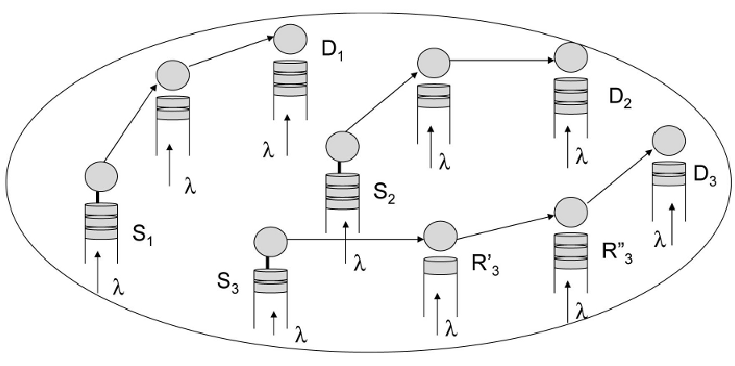
\includegraphics[scale=0.4]{./graph/rb_queue.png}
\caption{Rezervēšanas komutācijas modelis \cite{route_res}.}
\label{fig:rb}
\end{figure}

Laikā kamēr mezgls ir iesaistīts daudzposmu maršrutā, tas retranslē datus tikai vienam avotam. No kā izriet, ka visi aktīvi daudzposmu maršruti ir sašķelti. Tātad, pie vidējā daudzposmu maršruta garuma $\bar{n_{h}}$ tīklā ar $N$ mezgliem var būt maksimālais aktīvu maršrutu skaits $C_{s}$. Sašķeltu maršrutu $C_{s}$ skaitu var izteikt kā \cite{route_res}
\begin{equation}
C_{s}\simeq \frac{N}{\bar{n}_{h}+1}
\end{equation}
Ja mezglu skaits, kas vēlas izveidot daudzposma maršrutus ir lielāks par $C_{s}$, tad dažiem mezgliem būs jāgaida noteikts laika periods pirms tie vārēs izveidot maršrutu.
\begin{figure}[htb!]
\centering
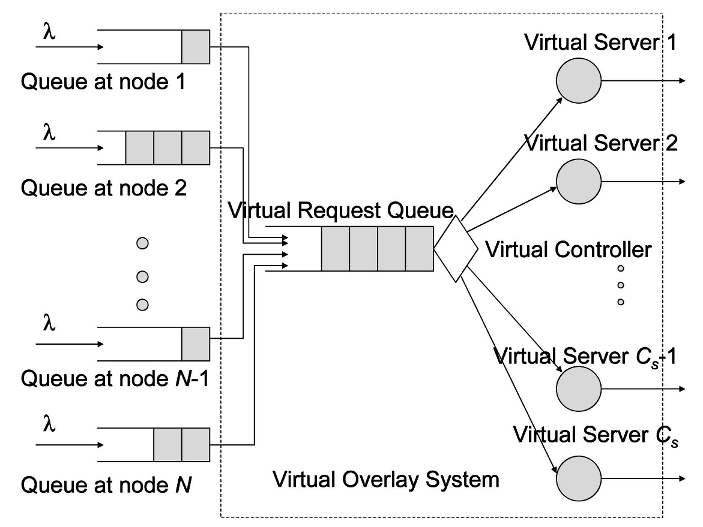
\includegraphics[scale=0.4]{./graph/rb}
\caption{Rindas veidošanās  MANET ar rezervēšanas komutāciju, \cite{route_res}}
\label{fig:rbServer}
\end{figure}

RB modelī maršruta izveidošanas procesu var aprakstīt ar \textit{virtuālā pieprasījumu rindu} (\seename ~\figurename.
~\ref{fig:rbServer} ''virtual request queue''), kas pārvalda pieprasījumus no visiem avotiem. Pirmais ziņojums no katra avota buferī nekavējoties tiek pārsūtīts uz \textit{virtuālā pieprasījuma rindu}. Ar \textit{virtuālā pieprasījuma rindas} paņēmienu modelē gaidīšanas laiku, tas ir laiks kuru avotam jāgaida sākot no maršruta izveidošanas brīža līdz momentam, kad avots vārēs aktīvi to izmantot. Katrs iespējamais daudzposmu maršruts atbilsts virtuālajam serverim (\seename ~\figurename. ~\ref{fig:rbServer} ''virtual server'') un katrs serveris pārvalda ziņojumus \textit{virtuālā pieprasījumu rindā}. Serveru skaits atbilst šā tīkla maksimālajam aktīvu maršrutu skaitam $C_{s}$. Laiks, kuru ziņojums pavada \textit{virtuālā pieprasījumu rindā}, ir vienāds ar laiku kas ir nepieciešams retranslācijas mezgliem, lai tie atkal kļūtu pieejami. Tādēļ ziņojumi, kas atrodas \textit{virtuālo pieprasījumu rindā} netiek apstrādāti tādā pašā secībā, kādā tie tika saņemti.\\
Papildus informāciju par RB komutāciju un to modeļu aprēķiniem var atrast O.K.Tongus darbā  \cite{route_res}.


\subsection{Bez rezervēšanas komutācija}\label{sec:nrbs}
Bez rezervēšanas komutācijas (\acs{NRBS}) modelī, pirms datu pārraides nav iepriekšējas retranslējošo mezglu rezervēšanas. Retranslējošie mezgli var vienlaicīgi piedalīties vairākos daudzposmu maršrutos. Att. \ref{fig:nrb} pāradīti divi iespējamie maršruti starp $S_{1}$ un $D_{1}$ (pārtraukta līnija, un pārtraukta-punktaina līnija). Ir redzams, ka viens un tas pats avots $S_{3}$ var vienlaicīgi pārraidīt ziņojumus uz diviem dažādiem galamērķiem $D_{3}$ un $D_{3}^{'}$.

\begin{figure}[htb!]
\centering
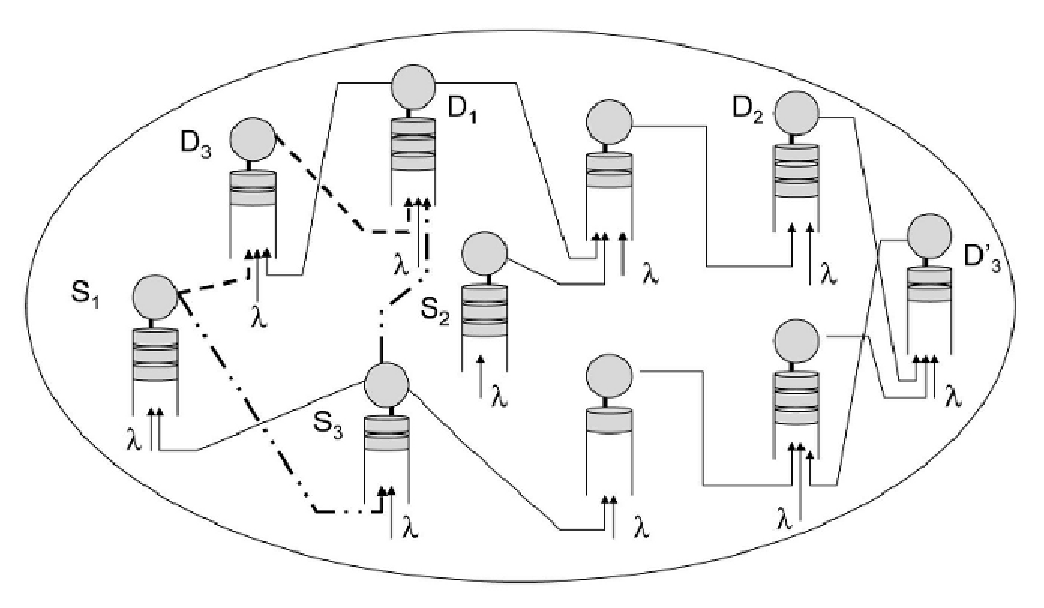
\includegraphics[scale=0.4]{./graph/nrb}
\caption{Bez rezervēšanas komutācijas modelis \cite{route_res}}
\label{fig:nrb}
\end{figure}

Kad $n_{a}$ mezgls saņem ziņojumu no $n_{b}$ mezgla ($n_{a}$ darbojas kā releja), $n_{a}$ ievieto saņemto ziņojumu bufera rindā kopā ar $n_{a}$ mezgla ģenerētiem ziņojumiem. Ziņojumi no šīs rindas tiek pārraidīti secīgi, saņemtiem un $n_{a}$ ģenerētiem ziņojumiem nav prioritātēs šajā rindā.
Šī ir \acs{NRBS} pamatatšķirība no \acs{RBS} komutācijas modeļa, kurā retranslējoši mezgli dod absolūtu prioritāti saņemtiem ziņojumiem un savu ziņojumu pārraidi pilnībā aptur. \ac{NRBS} modelī katrs daudzposma maršruts ir rindu tandēms un visu tīklu var uzskatīt kā rindu tandēmu (\figurename. ~\ref{fig:nrbTandem}).

\begin{figure}[htb!]
\centering
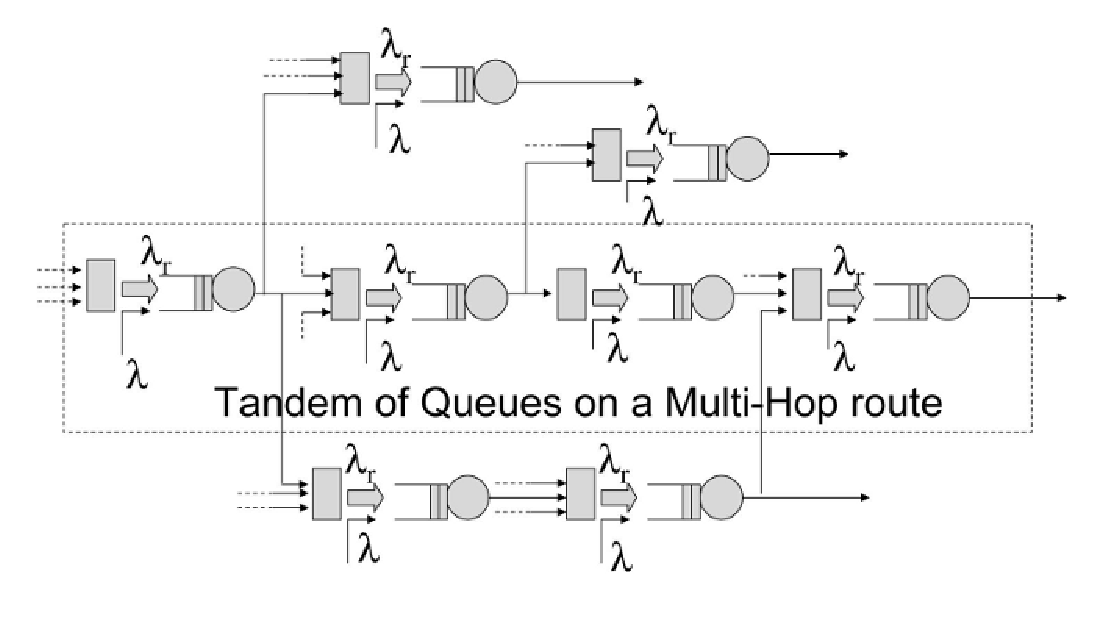
\includegraphics[scale=0.4]{./graph/tandem}
\caption{ Bez rezervēšanas komutācijas tandēmrinda \cite{route_res}}
\label{fig:nrbTandem}
\end{figure}

% \subsection{ Mobilitātes ietekme uz komutācijas modeļa veiktspēju}
% Pieņemsim, ka mobilie mezgli 1) pārvietojas ierobežota un konstanta pēc izmēra laukumā $A$ 2) vienmēr var atrast kaimiņ-mezglu uz $\Theta(1/\sqrt{\rho A})$ attālumā. Jāatzīmē ka, pastāv iespēja ka $\Theta(1/\sqrt{\rho A})$ attālumā kaimiņ-mezgls nav nekavējoties pieejams; tas izraisa pārraides aizkāvi no avota līdz galamērķim. Tīklā ar \ac{RBS} komutāciju savienojuma garums starp mobiliem mezgliem var paliecināties laikā un tas ietekmes tīkla robustumu. \ac{RBS} robustums ir daudzkārtēji mazināts ar mezglu mobilitāti salīdzinājumā ar \ac{NRBS}. Tīklā ar \ac{NRBS} komutāciju kad pārraide no avota ir sākusies  maršruta secīgas savienojuma izvēlēti  oportūnistiski, balstoties uz attāluma. Gadījuma ja divi noteikta maršruta secīgi mezgli pārāk attālinās viens no otra, savienojuma sakuma mezgls ( mezgls kas secīgi ir pirmais) izvēlas citu mezglu kas atrodas $\Theta(\sqrt{1/\rho A})$ attālumā. Lai nodrošināt šādu maršruta izveidi ir nepieciešama liela vadības ziņojumu (control message) apmaiņa starp retranslējošiem mezgliem.

\chapter{Mobilitātes Modeļi}\label{sec:mobilityModels}
Mobilitātes modelis ir noteikumu kopa, kas nosaka mobilas vienības trajektoriju \cite{tuduce}. Modelim jāatbilst sekojošiem  kritērijiem:
\begin{itemize}
\item jābūt iespējai apvienot kopā n modeļus un izveidot tādu pašu lielāka izmēra modeļus
\item jābūt mainīgiem lielumiem, kurus mainot var izveidot dažādus mobilitātes  scenārijus
\item modelim jābūt stacionārai
\item modelim nepieciešams nekorelēt
\end{itemize}

Pamatmetode ar kuru pēta ekspromta tīklu darbību un procesus ir datorsimulācija (turpmāk simulācija). Simulācijai ir vairākas būtiskas priekšrocības: iespēja identiski atkārtot scenāriju, iespēja izolēt noteiktus parametrus un iespējams variēt dažādus tīkla raksturlielumus. Mobilo Ad Hoc un WSN tīklu simulācijā galvenie faktori ir tīkla topoloģija un mezglu kustība, kas ietekmē pētāmā tīkla parametrus. Tīkla topoloģija nosaka mezglu sākotnējo izvietojumu, savukārt mobilitātes modelis nosaka mezglu kustību tīklā. Mezglu mobilitātes modelis visvairāk ietekmē maršrutēšanas protokola darbību. Simulācijas rezultāti, kas iegūti ar nekorektu mobilitātes modeli izveido nepareizu priekšstatu  par protokolu darbību un par tīklā notiekošiem procesiem.

Mobilitātes modeļi tiek uzskatīti par vienu no lielākajām problēmām mobilo ekspromta tīklu simulācijas jomā \cite{tuduce}. Reālas pasaules lietotāju uzvedības modelēšana ir sarežģīts uzdevums un bieži rodas nepieciešamība izvēlēties kompromisu starp modeļa sarežģītību un precizitāti. Viens no paņēmieniem ir novērot mobilitātes modeli (tā rakstu) reālā sistēmā. Tomēr metode nav pilnībā efektīva, jo tā atspoguļo tikai vienu kustības scenāriju, kuru nav iespējams vispārināt. Turklāt, šādi modeļi neatbilst iepriekš minētajam kritērijam, proti modelim ir jābūt stacionārām, jo lietotāju kustība un daudzums ir atkarīgs no diennakts laika. Piemēram, lielveikala apmeklētāju skaits diennakts laikā  var svārsties no 0 apmeklētājiem naktī, līdz simtiem apmeklētāju pīķa stundās. Risinājums ir mākslīgie modeļi (synthetic models), kas plaši tiek  pielietoti daudzos pētnieciskos projektos. Vairums no šobrīd visplašāk sastopamajiem mākslīgajiem modeļiem ir aprakstīti Camp darbā \cite{camp}. Šajā nodaļā tiks apskatīti trīs visbiežāk pielietojamie modeļi: \acf{RWMM}, \acf{RDMM} un \acf{OMM}. Šie modeļi ir pieejami \acl{NS-2} un GloMoSim datorsimulāciju programmās.

\begin{figure}[htb!]
\begin{minipage}[t]{0.45\linewidth}
\centering
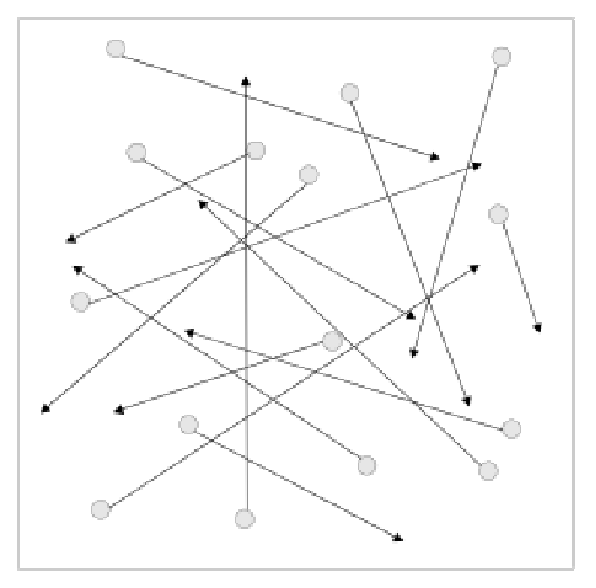
\includegraphics[scale=0.45]{./graph/RWMM1}
\caption{Gadījuma maršrutpunktu mobilitātes modelis (RWMM)} \label{fig:rwmm}
\end{minipage}%
\hspace{0.5in}
\begin{minipage}[t]{0.45\linewidth}
\centering
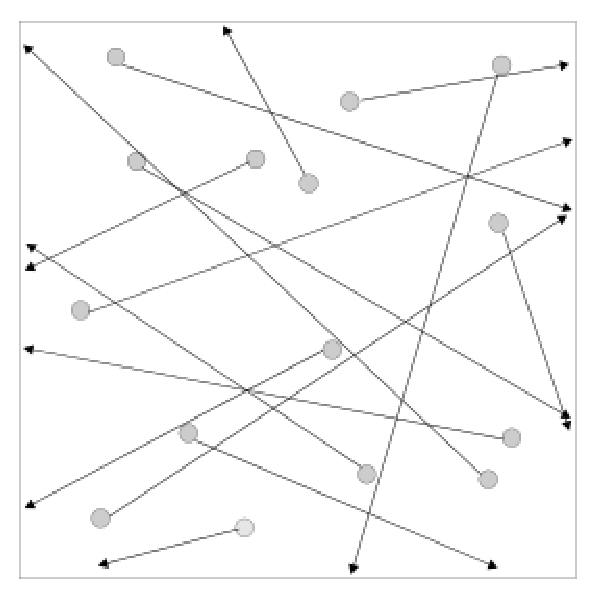
\includegraphics[scale=0.45]{./graph/RWMM2}
\caption{Gadījuma virzienu mobilitātes modelis (RDMM)} \label{fig:rdmm}
\end{minipage}
\end{figure}

\section{Mobilitātes modeļu raksturlielumi}
Ja tīklu apskata no simulācijas viedokļa, tad mobilitātes modeļi būtībā atšķiras pēc mezglu sākotnējas izvietošanas tīkla laukumā $S^{2}$ un ar mezglu izmaņu simulācijas laikā. Lai modeli raks-turot matemātiski, izmanto telpisko mezglu izvietošanu laukumā. Lai simulācijas mērķis būtu ar pēc iespējās reālistisku scenāriju, tad ir jāņem vērā arī: mezglu kustības ātrumu, savienojuma ilgumu, mezglu izkliedi un to blīvumu tīkla laukumā.

\subsection{Atkarība starp tīkla laukumu un mezglu ātrumu}
Sākuma mezglu izvietojums un ātrums nosaka vēlāko mezglu izvietojumu simulācijas laukumā. Turklāt izvietošanas un ātruma varbūtības sadalījums nepārtraukti mainās laika gaitā. To - kādā laika brīdī tīkls sasniegs savu 'līdzsvara' stāvokli, matemātiski var aprakstīt ar stacionāro sadalījumu \cite{navid}.

\subsection{Savienojuma ilgums}
Savienojuma ilgums ir laika periods starp savienojuma izveidi līdz tā izjaukšanai. Simulācijas vidējais savienojuma ilgums ir vidējais aritmētiskais no visiem savienojumiem, kas tiek izveidoti simulācijas laikā. Šis parametrs ir svarīgs jo mēdz gadīties, ka protokoli, kuriem ir nepieciešams platjoslas savienojums, nebūs spējīgi darboties īslaicīgā savienojuma dēļ.

Bieži vien simulāciju programmās tiek pieņemts, ka savienojums izveidojas tiklīdz mezgli ir viens otra uztveres diapazonā (attālums starp mezgliem $\leq$ \gls{r_link}). Reālajā dzīve tā nav, jo brīdī, kad mezgls konstatē elektromagnētiskā signāla klātbūtni, pirms komunikācijas uzsākšanas ar raidītājmezglu,  tam ir nepieciešams sinhronizēties. Piemēram, ierīcēm ar Bluetooth tehnoloģiju ir nepieciešamas aptuveni 10 sekundes, lai divi mezgli uztveres diapazonā izveidotu savienojumu. Ņemot vēra šo faktu, kā arī to, ka mezgli kustas ātri, pastāv ļoti augsta varbūtība gadījumam, ka $r_{link}$ attālumā atrodošies divi mezgli, kas ātri kustas pretējos virzienos, nevarēs izveidot savienojumu (pat ja kādā brīdī tie būs ļoti tuvu). Tas ir tādēļ, ka laiks, kas ir nepieciešams savienojuma izveidošanai ir lielāks par laiku, kurā tiek šķērsota distance $r_{link}$.

\subsection{Mezglu blīvums}
$A$ mezglā kaimiņ-mezglu blīvums ir mezglu skaits kas atrodas $A$ mezgla uztveres diapazonā. Tīklā, kur telpiskais sadalījums ir viendabīgs, vidējais kaimiņ-mezglu blīvums ir būtisks parametrs. Aprēķina pēc (\ref{eq:blivums}) formulas.

\subsection{Mezglu izkliede}
Mezglu blīvums arī saukts par telpisko blīvums, ir mezglam $A$ kaimiņ-mezglu skaits $y$ uz laukuma vienību, šos kaimiņus var sadalīt $i$ dažādās kārtās (\seename~\figurename. ~\ref{fig:topo}) un aprēķina kā $\rho_{s}=\frac{N}{A}$. Ja mezglu skaits pirmajā kārtā ir $k$, tas nozīme ka sadalījums $D(k)$ ļauj izvēlētajam mezglam $A$ izveidot $k$ skaitu savienojumu. Dalījums kārtās sniedz iespēju iegūt informāciju par to vai mezglam $A$ būs iespējams izveidot savienojumu vai nē. Jo augstāka mezglu izkliede tīklā, jo augstāka ir varbūtība, ka mezgls $A$ izveidos 0 savienojumu.


\section{Gadījuma maršrutpunktu mobilitātes modelis}
Gadījuma maršrutpunktu mobilitātes modelis (\acs{RWMM}) ir viens no vienkāršākajiem un arī visplašāk pielietojamais mobilo Ad Hoc tīklu simulēšanai. Gadījuma maršrutpunktu mobilitātes modelī katram mezglam ir noteikts izvietojums (\seename~\figurename.~\ref{fig:rwmm}). Pārraides laikā ātrums \gls{v} un kustības virziens nemainās. Mezgla kustības galamērķis ir nejauši izvēlēta vieta tīkla laukumā. Ātrums $v$ ir izvēlēts intervālā $(v_{min}, v_{max})$, neatkarīgi no mezgla sākotnējās pozīcijas un tā kustības galamērķa. RWMM minimālais ātrums $v_{min}$ var būt tikai pozitīvs skaitlis, pretējā gadījumā vidējais ātrums būs negatīvs lielums. Kad mezgls nonāk galamērķī, tas var izdarīt pārtraukumu uz nejauši izvēlētu laiku, vai arī turpināt kustību uz jauno galamērķi. Mezglam tiek piešķirts jauns galamērķis un jauns ātrums $v$ neatkarīgi no iepriekšējā ātruma, galamērķa un pārtraukuma izvēles. Simulēšanas procesā RWMM mezglu izvietojums un ātrums neatbilst vienveidīgam izkārtojumam. Novērots, ka stacionārs mezglu izkārtojums tiek koncentrēts ap tīkla centru (\seename~\figurename.~\ref{fig:rwmm}), kurā notiek aktīva mezglu kustība \citep{bett, navid}.

\section{Mobilitātes modeļa ietekme uz BER}
Mezglu mobilitāte var tikt raksturota ar  ātrumu $v$ un tā leņķi \gls{theta} (leņķis attiecībā pret horizontālo asi). Gadījuma maršrutpunktu mobilitātes modelī (\acs{RWMM}) ziņojuma pārraides laikā, divu pārraidē iesaistītu mezglu ātrums un kustības virziens paliek nemainīgs.
\subsection{Scenārijs ar RWMM un NRBS}
Tiek uzskatīts, ka daudzposmu maršrutā secīgie posmi ir neatkarīgie viens no otra. Katrā no diviem posmiem vienā un tajā pašā maršrutā, mezgla beigu pozīcija (savienojumā, kur tas ir uztvērējs) būs neatkarīga no tā paša mezgla pozīcijas nākošā posma sākumā (jaunajā savienojumā, kur tas ir raidītājs). Mezgli $n_{A}$ un $n_{B}$ ir mezglu pāris kurš veido savienojumu. Ziņojuma pārraides laikā abiem mezgliem ātrums un virziena leņķis ir konstantes, $(v_{A}, \theta_{B})$ un $(v_{B}, \theta_{B})$. Sākotnējā pozīcijā mezgli $n_{A}$ un $n_{B}$ atrodas $r_{link}$ attālumā. Att.~\ref{fig:dp} ilustrēts kā mainās savienojuma garums $r_{link}$ a) pārraides sākumā $t_{s}$ un b) pēc ziņojuma pārraides $t_{e}=t_{s}+t_{msg}$.

\begin{figure}[!htb]
\centering
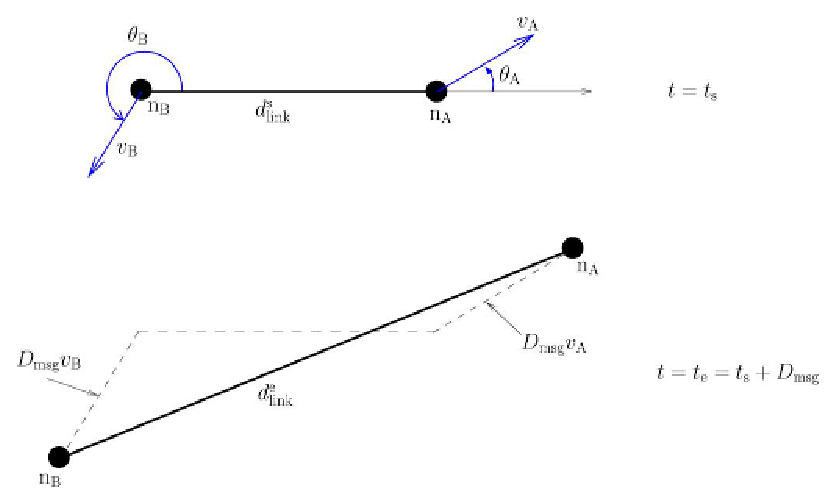
\includegraphics[scale=0.65]{./graph/dp}
\caption{Mezgla kustības trajektorija ar RWMM pie NRBS \cite{qoS_mobility}}
\label{fig:dp}
\end{figure}
Pielietojot kosinusu teorēmu posma garums $r_{link}^{e}$ laika bridī $t_{e}$ būs
\begin{align}
r_{link}^{e} &= \left[ r_{link}^{2} + t^{2}_{msg}(v^{2}_{A}+v^{2}_{B})-2v_{A}v_{B}t^{2}_{msg}cos(\theta_{A}-\theta_{B})+ \right. \nonumber \\
    &\qquad {}\left.	+2r_{link}t_{msg}(v_{A}cos\theta_{A}-v_{B}cos\theta_{B})\right]^{\frac{1}{2}}
\end{align}
Tātad, divu mobilu mezglu vidējais maršruta posma garums $\bar{r}_{link}$ ir vienāds ar $\bar{r}_{link}=\frac{1}{2}(r_{link}+r_{link}^{e})$. Lai aprēķinātu SNR pārraides laikā var izmantot (\ref{eq:snr}) formulu, aizvietojot $r_{link}$ ar $\bar{d}_{link}$. Pamatatšķirība ar statiska tīkla ir tā, ka $\bar{d}_{link}$ ir gadījuma lielums, kas ir atkarīgs no $(v_{A}, \theta_{A})$ un $(v_{B}, \theta_{B})$.

Vienkāršībai, tiek uzskatīts, ka katra mezgla kustības veids ir neatkarīgs no pārējiem mezgliem. Ziņojuma pārraides laikā daudzposmu maršruta $i$-tās posma ($i \in {1,\cdots ,\bar{n}_{h}}$), divu mezglu ātrums un kustības virziens ir $\zeta_{i}=(v_{i},\theta_{i},v_{i+1}, \theta_{i+1})$. Kur divi secīgi stāvokļi $(v_{B},\theta_{B})$ un $(v_{A}, \theta_{A})$ attiecas uz vienu un to pašu mezglu. Šis pieņēmums neietekmē savienojumu posmu skaitu daudzposmu maršrutā \cite{qoS_mobility}. Acīmredzams, ka $\bar{r}_{link} = r_{link}(\zeta_{i})$ un $i$-tā lēkuma BER būs $BER_{link}(\zeta_{i})$. Tādēļ daudzposmu maršruta galā $BER_{route}$ ar vidējo lēkumu skaitu $\bar{n}_{h}$ un pie $\zeta_{NRBS}=(\zeta_{1}, \cdots,\zeta_{\bar{n}_{h}})$ būs \cite{qoS_mobility}
\begin{equation}
BER_{route}(\zeta_{NRBS})=1-\prod_{i=1}^{\bar{n}_{h}}\left[1-BER_{link}(\zeta_{i})\right].
\end{equation}
Pie pietiekami liela realizāciju skaita $\eta$, $\zeta_{NRBS}^{j}=(\zeta^{j}_{1}, \cdots,\zeta^{j}_{\bar{n}_{h}}), j\in[1, \cdots,\eta]$ vidējais BER būs \cite{qoS_mobility}
\begin{equation}
BER_{route}=\frac{\sum_{j=1}^{\eta}BER_{route}\left(\zeta_{NRBS}^{j}\right)}{\eta}.
\end{equation}


\subsection{Scenārijs ar RWMM un RBS}
Pēc maršruta izveides, ziņojums 'plūst' caur iepriekš rezervētiem maršruta posmiem neatkarīgi no pārmaiņām tajā un mobilitātes iespaida. Att. ~\ref{fig:dpRBS} ilustrēta mezglu mobilitātes ietekme uz iepriekš rezervētu maršrutu. Attēlā, kad $t=t_{1}+5\times t_{msg}$ var redzēt, kā maršruts izliecas ap $n_{3}$ mezglu. Maršrutu iespējams pilnveidot izslēdzot $n_{3}$ no maršruta, jo mezgli $n_{2}$ un $n_{4}$ var komunicēt pa tiešo. Acīmredzams, ka - jo lielāks mezglu ātrums $v_{i}$, jo ātrāk notiks savienojuma posma pārrāvums.

\begin{figure}
\centering

\includegraphics[scale=0.40]{./graph/dpRBS.png}
\caption{Maršruta izmaiņas pārraides laikā ar RBS \cite{qoS_mobility}}
\label{fig:dpRBS}
\end{figure}

Tā kā RBS iepriekš rezervē mezglus visa maršruta garumā un tas nemainās visas pārraides laikā, tad mēs varam uzreiz aprēķināt visa maršruta garuma izmaiņas. Maršruts sastāv no $i$ savienojumiem posmā starp $n_{i}$ un $n_{i+1}$ mezgliem, ziņojuma pārraides laikā $t = t_{1}+(i-1)t_{msg}$, sākuma un beigu maršruta garumi var tikt izteikti\footnote{Balstīts uz pieņēmuma, ka starp diviem kaimiņ-mezgliem izplatīšanās laiks ir niecīgs, salīdzinot ar visa ziņojuma pārraides laiku. Šis pieņēmums ir patiess visa veida sensoru tīkliem, kuros veiksmīgi izveidoti savienojumi starp kaimiņ-mezgliem.}, kā \cite{qoS_mobility}:

\begin{align}
  r_{link}^{i,s} &= \left[ r_{link}^{2} + ((i-1)t_{msg})^{2}(v_{i}^{2} + v_{i+1}^{2})-2v_{i}v_{i+1}((i-1)t_{msg})^{2}cos(\theta_{i}-\theta_{i+1})+ \right.\nonumber \\
    &\qquad {} \left.  +2r_{link}(i-1)t_{msg}(v_{i}cos\theta_{i}-v_{i+1}cos\theta_{i+1})\right]^{\frac{1}{2}} 	\nonumber
\end{align}
\begin{align}
  r_{link}^{i,e} &=\left[ r_{link}^{2} + (it_{msg})^{2}(v_{i}^{2} + v_{i+1}^{2})- 2v_{i}v_{i+1}(it_{msg})^{2}cos(\theta_{i}-\theta_{i+1})+ \right.\nonumber \\
     &\qquad {} \left.  +2r_{link}i t_{msg}(v_{i}cos\theta_{i} - v_{i+1}cos\theta_{i+1}) \right]^{\frac{1}{2}}  \nonumber
\end{align}

Tātad, vidējo maršruta garumu var aprēķināt kā aritmētisko vidējo no sākuma un beigu garumiem $\bar{r}_{link}^{i} = (r_{link}^{i,s}+r_{link}^{i,e})/2$.

BER $i$-tā savienojuma posma beigas var izteikt izmantojot (\ref{eq:BER_routeProd}) formulu, aizvietojot $r_{link}$ ar $\bar{r}_{link}^{i}$, kas ir atkarīgs no $(v_{i}, \theta_{i})$ un $(v_{i+1}, \theta{i+1})$. Un vidējais maršruta posmu skaits ir $[\bar{r}_{link}^{1},\cdots, \bar{r}_{link}^{\bar{n}_{h}}]$, kas ir atkarīgs arī no realizēto mezglu kustībām $\zeta_{RBS} = [(v_{1},\theta_{1}),\cdots ,(v_{\bar{n}_{h}}, \theta_{\bar{n}_{h}})]$.

Vienkāršība laba tiek uzskatīts, ka katra mezgla kustības veids ir neatkarīgs no pārējiem mezgliem. Ziņojuma pārraides laikā daudzposmu maršruts ar $i$ savienojumiem ($i \in {1,\cdots ,\bar{n}_{h}}$) divu mezglu ātrums un kustības virziens ir $\zeta_{i} = (v_{i},\theta_{i},v_{i+1}, \theta_{i+1})$. Tādēļ daudzposmu maršruta galā $BER_{route}$ ar viduvēju lēkumu skaitu $\bar{n}_{h}$ un $\zeta_{RBS}$ būs \cite{qoS_mobility}

\begin{equation}
BER_{route}(\zeta_{RBS}) = 1-\prod_{i=1}^{\bar{n}_{h}-1}\left[1-BER_{link i}(\zeta_{i})\right].
\end{equation}

Pie pietiekami liela realizāciju skaita $\eta$, $\zeta_{RBS}^{j} = [(v^{j}_{1}, \theta^{j}_{1}), \cdots,(v^{j}_{\bar{n}_{h}}, \theta^{j}_{\bar{n}_{h}})], j\in[1, \cdots,\eta]$ vidējais BER būs
\begin{equation}
BER_{route}=\frac{\sum_{j=1}^{\eta}BER_{route}\left(\zeta_{RBS}^{j}\right)}{\eta}.
\end{equation}

% \emph{\textbf{As at the end of the previous section, the final expression for the route BER is given by (19).}}


\section{Gadījuma virzienu mobilitātes modelis}
Gadījuma virzienu mobilitātes modelī (\acs{RDMM}) mezglu sākotnējā izvietošana tīkla laukumā ir vienveidīga un paliek nemainīga visas simulācijas laikā. RDMM mezgli maina kustības virzienu un ātrumu ziņojuma pārraides laikā. RDMM modelī mezglu kustība ir neatkarīgi un viendabīgi sadalīta (\acs{iid}), kustības virzienu maiņa notiek 'nepārtraukti' (laikā nepārtraukts stohastisks process). Mezglu kustības virzienu maiņa notiek laika periodos. Katrā laika periodā mezglam ir noteikts ātrums $v_{m}$ un virziens. Laikā perioda garums ir gadījuma lielums $p$, kas ir eksponenciāli sadalīts ar lielumu $\lambda_{m}$. Absolūti nepārtrauktu sadalījumu (\acs{CCDF}) $F_{m}(p)$ var izteikt kā \cite{camp}
\begin{equation}
F_{m}(p)=exp(-\lambda_{m}p)
\end{equation}

Katrā laika periodā kustības virziens (intervālā $[0, 2\pi)$) un ātrums $[v_{min}, v_{max}]$ ir vienmērīgi sadalīti. Ātrums, kustības virziens un perioda garums ir neatkarīgi katrā laika periodā. Turklāt, kad mezgls sasniedz šūnas robežu, tad mezgla kustības virziens tiek mainīts uz diametrāli pretējo, bet ātruma modulis paliek nemainīgs. Minimālais ātrums $v_{min}$ var būt nulle un pārtraukumā tas ir nulle.


\section{Šķēršļu mobilitātes modelis}
Šķēršļu mobilitātes modelis (\acs{OMM})  ir reālistisks mobilitātes modelis, kurā tīkla laukumā iekļauti šķēršļi \cite{jabra,jabras}. Šķēršļi ierobežo gan mezglu kustību, gan to signālu pārraidi (\seename ~\figurename. ~\ref{fig:omm1}). \acs{OMM} kustības trajektoriju izveidošanai izmanto Voronoi trajektorijas aprēķinu (Voronoi path computation) metodi\cite{aur}. Šķēršļu mobilitātes modelī šķēršļiem ir poligona forma, kas Voronoi diagrammu dala vienādās daļās (\seename ~\figurename. ~\ref{fig:omm2}). Tas dod iespēju aprēķināt Voronoi dalījumu skaitu simulācijas laukumā. Katrs Voronoi dalījums, kuram nav šķēršļa, tiek uzskatīts par iespējamo kustības trajektoriju.
 Mezgli var būt nejauši izvietoti segmentos izmantojot īsākā ceļa (short-path) metodi iespējams aprēķināt ceļu līdz galamērķim izvairoties no šķēršļiem.

\begin{figure}[htb!]
\begin{minipage}[t]{0.49\linewidth}
\centering
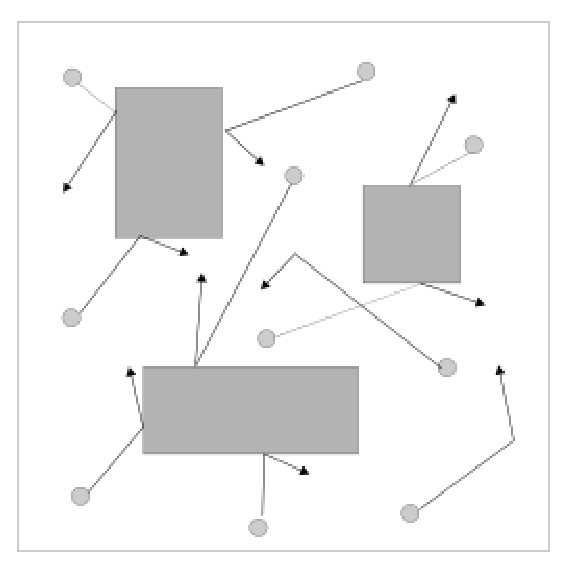
\includegraphics[scale=0.5]{./graph/OMM1}
\caption{Mobilo mezglu kustība laukumā ar šķēršļiem \cite{jabras}} \label{fig:omm1}
\end{minipage}%
\hspace{0.1cm}
\begin{minipage}[t]{0.49\linewidth}
\centering
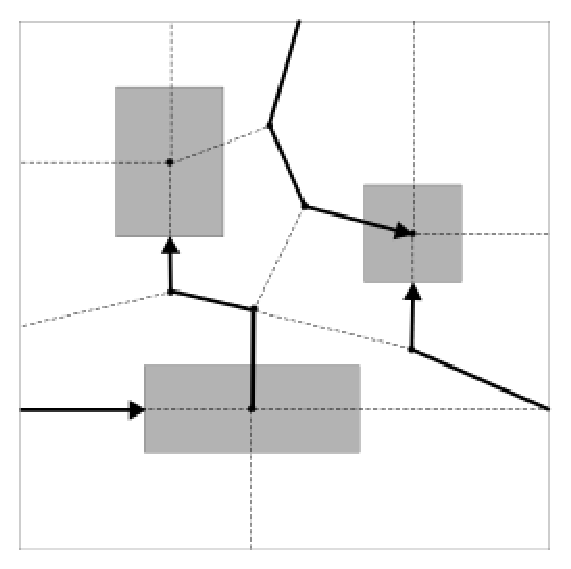
\includegraphics[scale=0.5]{./graph/OMM2}
\caption{OMM ar iepriekš noteiktiem kustības maršrutiem \cite{jabras}} \label{fig:omm2}
\end{minipage}
\end{figure}

Simulācijas rezultāti parāda, ka šķēršļu izmantošana un mezglu mobilitāte būtiski ietekmē ekspromta tīkla protokola veiktspēju \cite{jabras}.
\chapter{Maršrutēšanas protokoli}\label{sec:prot}
Mobilā WSN un Ad Hoc tīklā mezgli nepārtraukti kustās un raida informāciju. Lai atvieglotu maršruta izveides un uzturēšanas procesu tīklā tiek izmantoti maršrutēšanas protokoli. Abiem tīkliem maršrutēšanas protokola mērķis ir ātra un efektīva maršruta izveide un šo uzdevumu ir jāpaveic ar minimālu resursu patēriņu un joslas aizņemšanu. Kā tika minēts \ref{sec:infra} nodaļā, WSN atšķiras no MANET ar to, ka WSN tīklam ir limitēts enerģijas avots, kas arī ir kā uzstādījums un prasība maršrutēšanas protokoliem, taču tas neizslēdz iespēju ka abos tīklos var izmantot vienus un tos pašus protokolus.

Šajā nodaļā ir apskatīti trīs maršrutēšanas protokoli: DSR, AODV un OLSR un nodaļas noslēguma ir piedāvāts maršruta izvēles algoritma optimizācijas veids.

\section{Maršrutēšanas protokolu klasifikācija}
Maršrutēšanas protokolu klasificēšana var tikt izdarīta pēc sekojošiem principiem: \emph{A)} Distances vektora (distance vector) un posma stāvokļa (link state) maršrutēšana, \emph{B)} tabulu vadīta (Table driven) un sūtītāja vadīta (source driven) maršrutēšana un \emph{C)} pēc tīkla topoloģijas veida.

\begin{figure}[ht!]
\centering
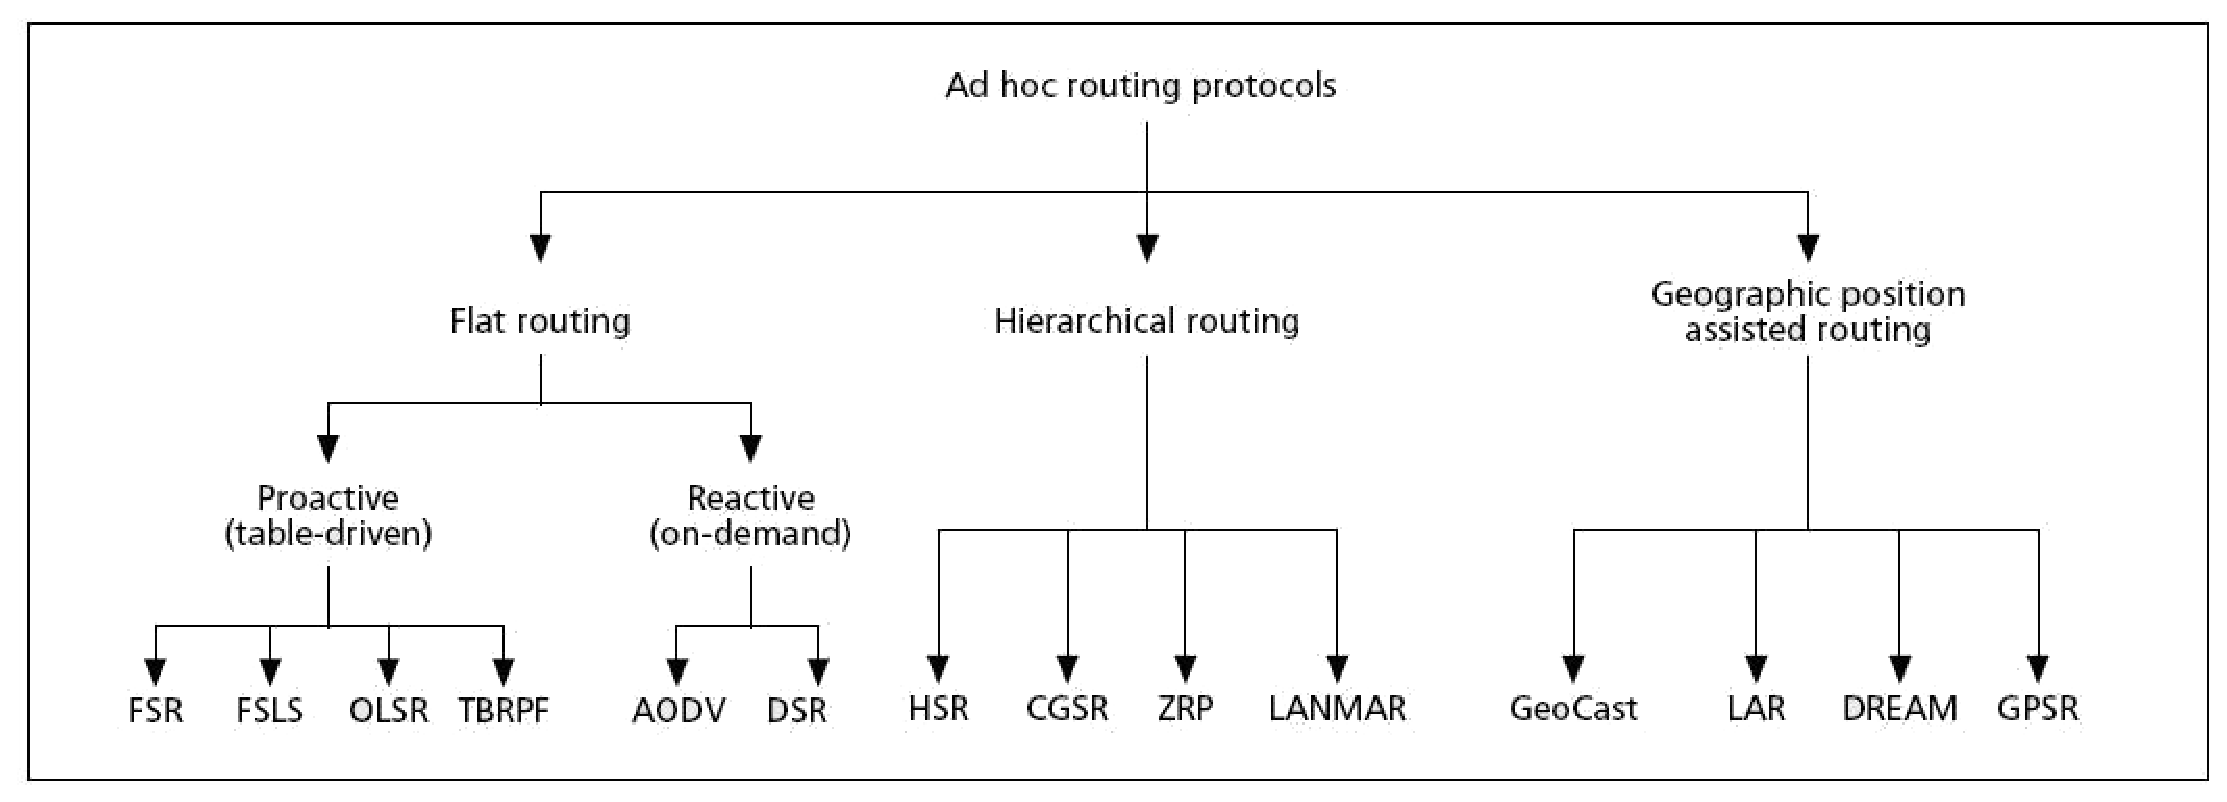
\includegraphics[scale=0.4]{./graph/protocol}
 \caption{Ad Hoc maršrutēšanas protokolu klasifikācija \cite{hong}}
\end{figure}

\textit{Distances vektora}  maršrutēšanas protokols ir balstīts uz decentralizēta algoritma. Katrs tīkla mezgls aprēķina īsāko maršrutu caur tiešiem kaimiņ-mezgliem (pirmās pakāpes kaimiņi) līdz pārējiem tīklā esošiem mezgliem (n-tās pakāpes kaimiņi). Šim maršrutēšanas veidam viens no būtiskākajiem trūkumiem ir: nevienam no mezgliem nav zināma globālā tīkla topoloģija, kā rezultātā ir nepieciešams ilgs laiks līdz visiem tīkla mezgliem ir vienādas ''zināšanas'' par apkārtējo topoloģiju. Att. \ref{fig:rout} a) ilustrē viena lēkuma (one-hop) maršrutu izplatīšanu ar distances vektora protokolu. Mezgla C pārraidītais distances vektors ļauj mezglam B aprēķināt attālumu līdz D kā $B \rightarrow D$ ir 2 un pārraidot šo informāciju A. Savukārt A distances vektors ļauj aprēķināt tā attālumu līdz D kā $A \rightarrow D$ ir 3.

\begin{figure}[ht!]
\centering
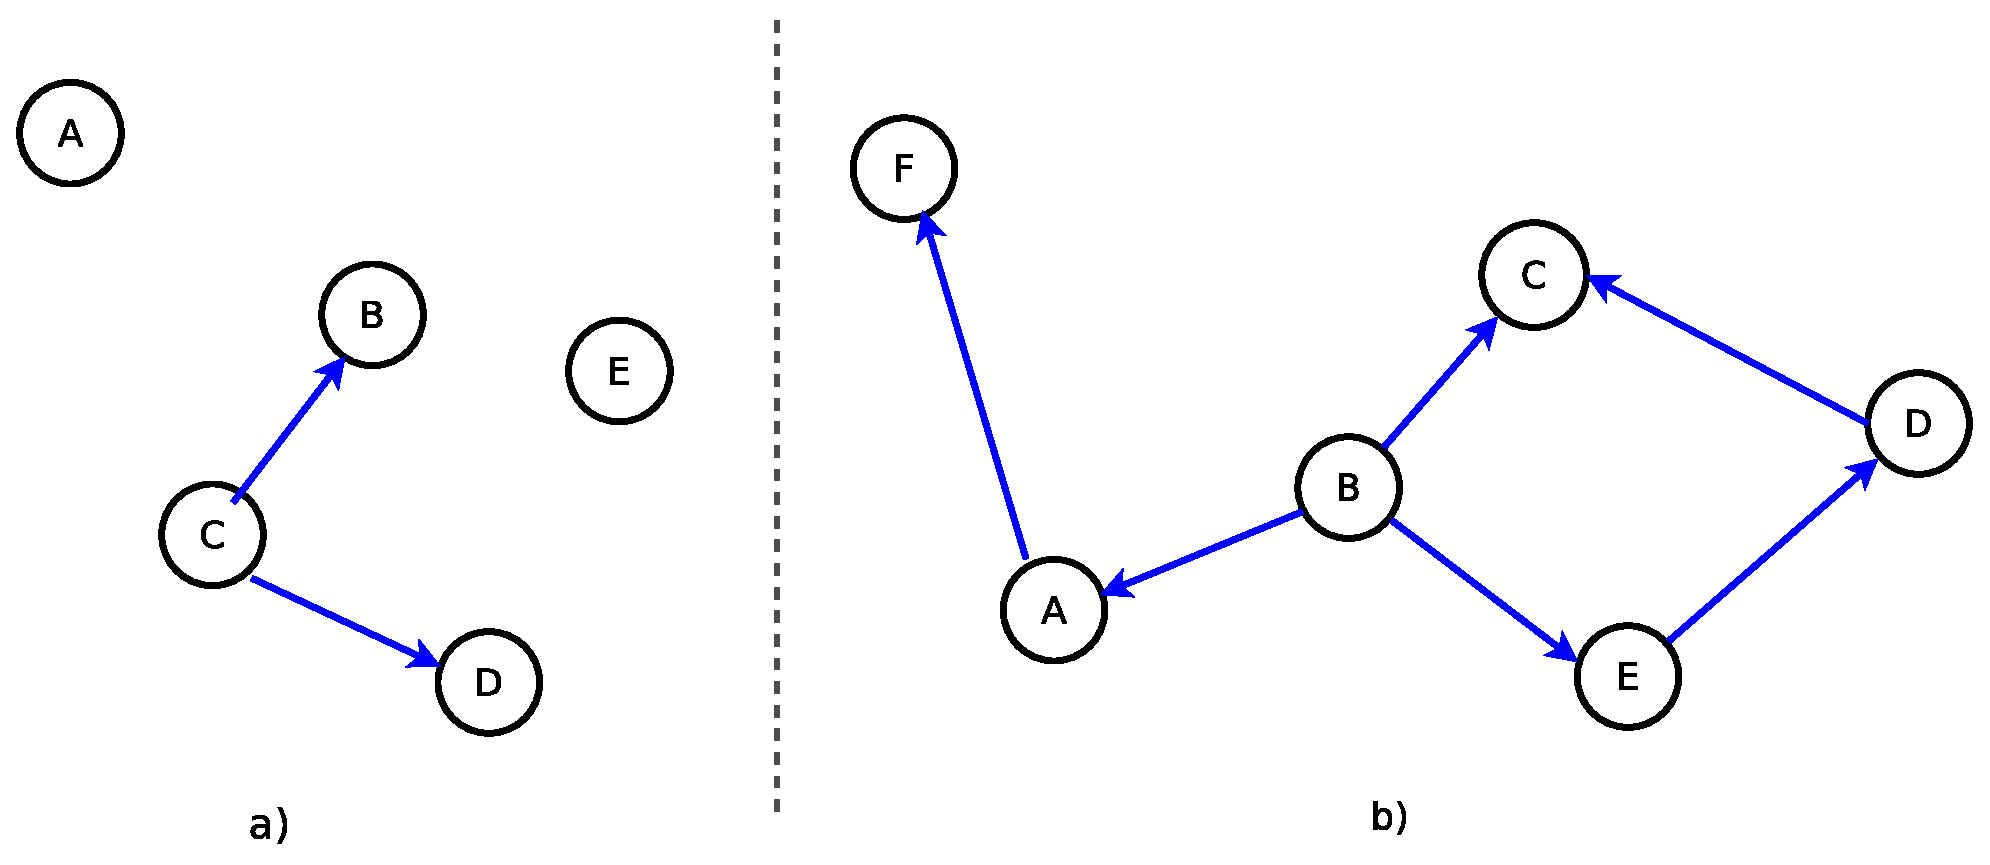
\includegraphics[scale=0.38]{./graph/dis_link}
 \caption{Maršruta atklāšana tīklā ar a) Distances vektora protokolu  un b) Posma stāvokļa protokolu}
\label{fig:rout}
\end{figure}

\textit{Posma stāvokļa} maršrutēšanas protokols balstīts uz globālā maršrutizēšanas algoritma. Katrs tīkla mezgls aprēķina īsāko maršrutu līdz ikvienam tīkla mezglam, tādā veidā iegūstot zināšanas par visiem iespējamajiem maršrutiem. Katrs mezgls pārraida posma stāvokli ikvienam tuvākajam kaimiņ-mezglam lai šī informācija tiktu tālāk pārraidīta visā tīklā. Šāda informācijas apmaiņa ļauj katram tīkla mezglam iegūt informāciju par visa tīkla topoloģiju. Att.\ref{fig:rout} b) ilustrē kaimiņ-mezglu informācijas izplatīšanu, izmantojot pārpludināšanas mehānismu (flooding mechanism). Divas posma stāvokļa paketes, viena no C un otra no B ļauj mezglam A noteikt tā maršrutu līdz mezglam D. \textit{Posma stāvokļa} algoritms salīdzinājumā ar \textit{Distances vektora} algoritmu tiek uzskatīts par labāku risinājumu, jo ļauj izvairīties no ''bezgalīgas skaitīšanas'' (count-to-infinity)\footnote{\emph{count-to-infinity} problēmas. Ja mezgls A informē mezglu B, ka tam ir maršruts līdz kaut kāda veida galamērķim, tad mezglam B nav iespējas uzzināt vai B ir daļa no tā vai nē.} un cilpošanas problēmām.

\textit{Tabulu vadītā} jeb \textit{Proaktīvā} maršrutēšanā. Protokols mēģina secīgi uzkrāt jaunāko informāciju par katru mezglu un izplatīt to katram tīkla mezglam. Protokols katrā mezglā saglabā vienu vai vairākas tabulas ar maršrutu informāciju un protokols reaģē uz tīkla topoloģijas izmaiņām ar atjauninājumu izplatīšanu visā tīklā, lai nodrošinātu konsekventu skatījumu par tīklu. Savā starpā \textit{Tabulu vadītie} protokoli atšķiras ar maršrutēšanai nepieciešamo tabulu skaitu un metodēm ar kurām tiek pārraidītas tīkla struktūras izmaiņas.

\textit{Sūtītāja vadīta} jeb \textit{Pēc pieprasījuma} (On-Demand) maršrutēšana izveido maršrutus tikai tad, kad to pieprasa sūtītāju mezgls. Kad mezglam ir nepieciešams maršruts līdz galamērķim, tas tīklā ierosina maršrutu atklāšanas (route discovery) procesu. Šo procesu var uzskatīt par pabeigtu tikai tādā gadījumā, ja maršruts ir atrasts vai visas iespējamās maršrutu permutācijas ir pārbaudītas.  Kad maršruts ir izveidots, tas tiek uzturēts ar maršrutu uzturēšanas procedūru līdz brīdim, kad galamērķis kļūst nepieejams izmantojot jebkuru no iespējamajiem maršrutiem, vai kamēr maršruta uzturēšana vairs nav nepieciešama.

Tīkla topoloģijas var izdalīt – ar vienotu maršrutēšanu (flat routing), hierarhisku maršrutēšanu (hierarchical routing) un maršrutēšana pēc ģeogrāfiskā izvietojuma (geographic position assisted routing)\cite{hong}. Saskaņā ar tīkla loģiskās struktūras organizēšanas nosacījumiem mobilie Ad Hoc maršrutēšanas protokoli var tik sadalīti uz a) klaster-bāzetiem (cluster-based), b) hierarhisku vai c) vienādranga struktūra, jeb d) hibrīd veida – apvienotā struktūra kas iekļauj abas iepriekš minētos struktūras veidus. Klaster-bāzēti protokoli pēc noteiktas loģikas iedala tīklu klasteros un katram klasterim piešķirot savu galveni. Visas galvenes savstarpēji uztur informāciju par tīkla globālo topoloģiju, šo informāciju galvenes izplata savā klasterī lai nodrošinātu pakešu pārsūtīšanu citiem klastera mezgliem. Vienādranga struktūras tīklā šāda tipa informācija apmaiņa nenotiek, kā rezultātā katram tīkla mezglam kešarmiņā ir jāuztur lokāla maršrutēšanas tabulu.



\section{DSR protokols}\label{sec:dsr}
Dinamiska avota maršrutēšanas protokols (\acs{DSR}) ir avota maršrutēts un maršrutēšanas protokols balstās uz avota iepriekšēju pieprasījumu.  Katrs mezgls kešatmiņā uzglabā maršrutu līdz tam zināmiem mezgliem. Šie dati tiek atjaunoti mezgla kešatmiņā tikai tad, kad tam kļūst zināmi jauni maršruti. Protokolam ir divas galvenās fāzes: maršruta atklāšana (route discovery) un maršruta uzturēšana (route maintenance).

Ja avota mezgls vēlās nosūtīt paketi adresātam, tad tas pārmeklē savu kešatmiņu lai pārliecinātos vai tam jau ir zināms maršruts līdz adresātam. Gadījumā, ja kešatmiņā esošā informācija par maršrutu līdz galamērķim vēl joprojām ir derīga, tad tas izmanto kešatmiņā pieejamo informāciju lai nosūtītu datus. Pretējā gadījumā avota mezgls iniciēs maršruta meklēšanas procesu ar maršruta pieprasījuma paketes (\acs{RREQ}) nosūtīšanu. RREQ satur avota  adresi, galamērķa adresi (varbūt daži) un unikālo idicifišanas numuru. Saņemot RREQ paketi katrs mezgls pārbauda savu kešatmiņu gadījumam vai tam jau ir zināms maršruts līdz galamērķim. Taču - ja starpmezglam nav zināms tāds maršruts, tad tas pievienos savu adresi paketes maršrutu sarakstā (route record) beigās un pārsūtīs to tālāk saviem kaimiņ-mezgliem. Lai ierobežotu RREQ pārsūtīšanas skaitu, mezgls analizē RREQ paketi tikai tādā gadījumā, ja mezgla adrese nav ierakstīta paketes zināmo maršrutu sarakstā. Attēlā ~\ref{fig:dsr} a) pāradīts kā pārvietojas RREQ un izveido maršrutu sarakstu (route record).
\begin{figure}[ht!]
\centering
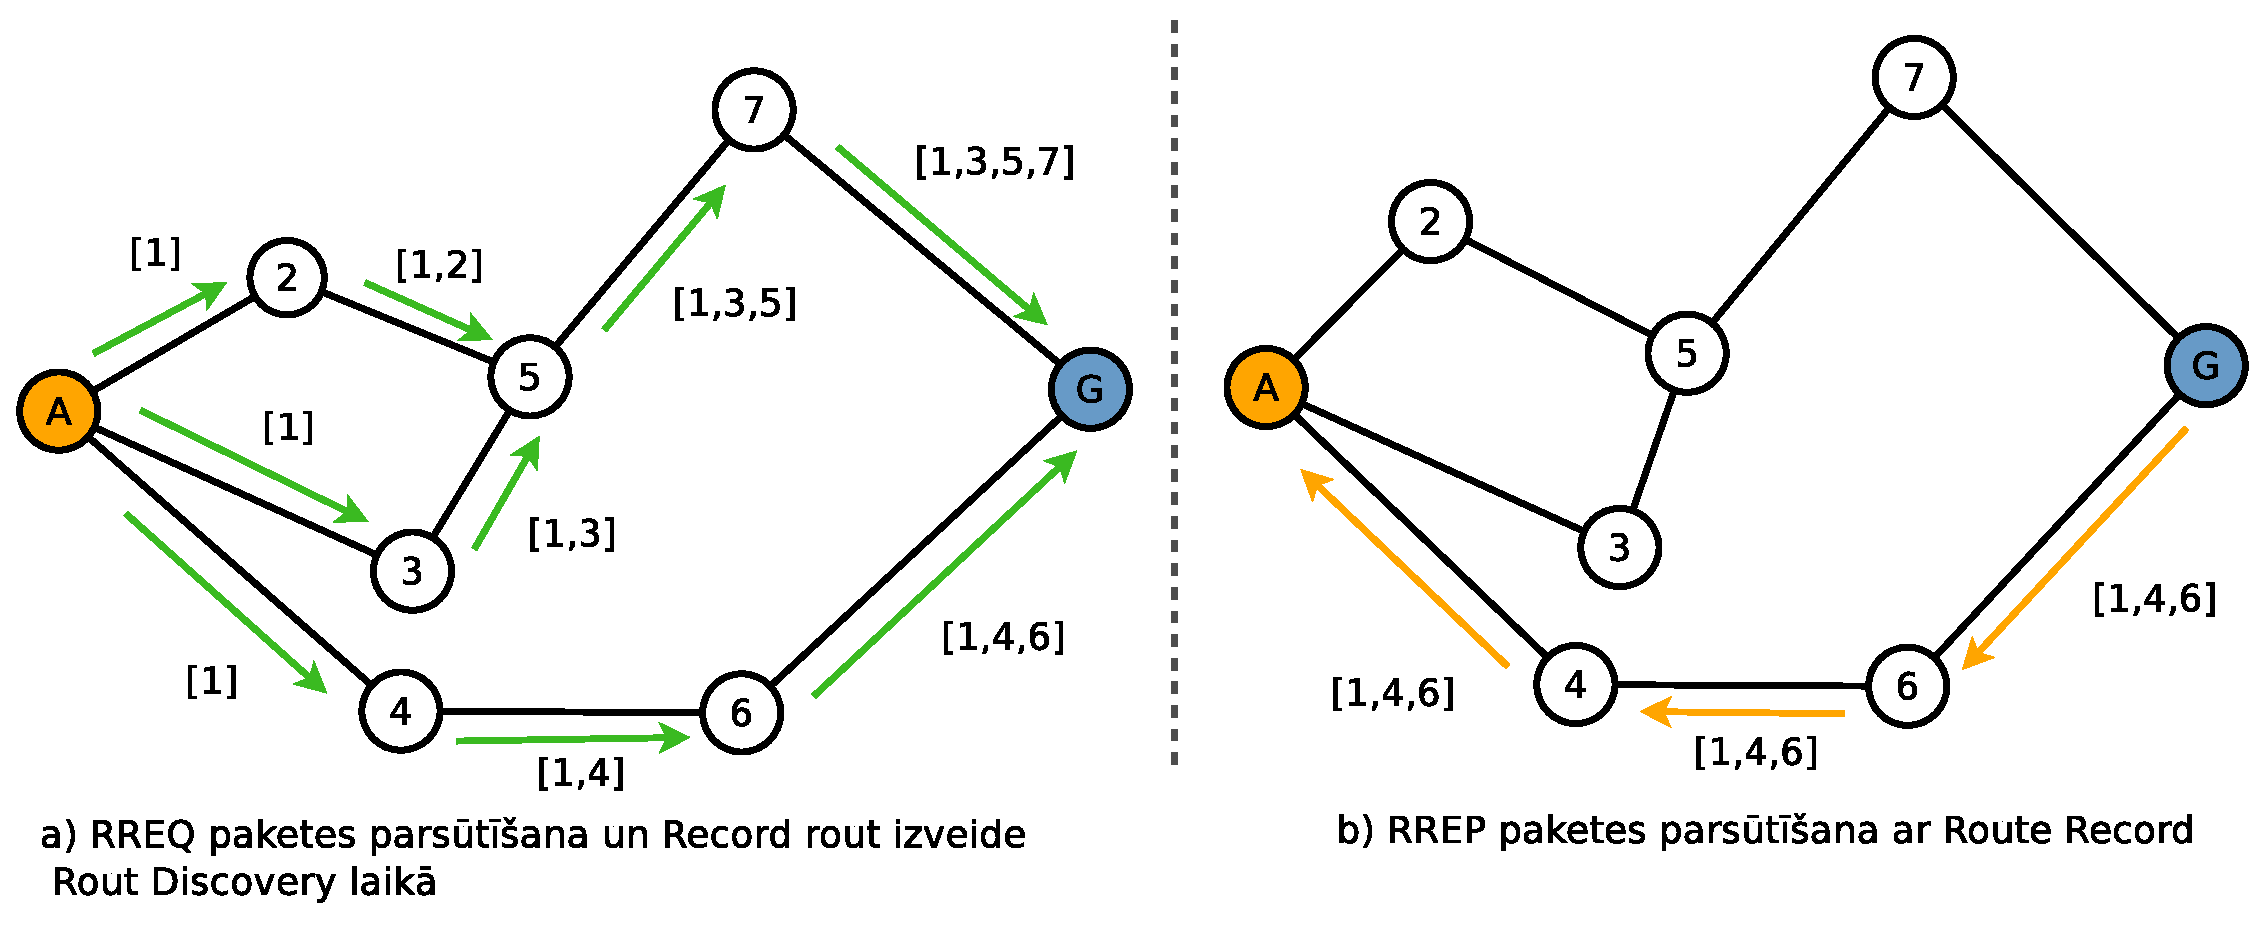
\includegraphics[scale=0.4]{./graph/dsr1}
 \caption{DSR protokola Route discovery}
\label{fig:dsr}
\end{figure}

\acf{RREP}  tiek izveidota ja RREQ sasniedz  galamērķi vai starp mezglu kuram ir informācija par maršrutu līdz galamērķim. Gadījumā ja RREQ sasniedz galamērķi, tad  galamērķis pārkopē maršruta sarakstu (informāciju  par ceļoto maršrutu) no RREQ uz RREP  paketi. Att.~\ref{fig:dsr} b) parādīts ka galamērķis pats nosūta RREP paketi.

Gadījumā kad RREP sasniedz starpmezglu, kuram ir zināma informācija par maršrutu līdz galamērķim, šis mezgls izveido RREP paketi. Mezgls iekopē maršruta sarakstu (route record) no RREQ paketes un pievino to kešatmiņas esošajam maršrutam beigās (RREP = kešatmiņas maršruts + route record). Mezgls var nosūtīt RREP paketi tikai tad, ja tam kešatmiņā ir maršruts līdz avotam. Ja mezglam šādas informācijas nav, tad tas iniciē maršruta atklāšanu (route discovery) līdz pat pašam avotam un pievieno RREP jaunajai RREQ paketei. Maršruta ieraksts (route record) no RREQ paketes var tikt izmantots tikai tādā gadījumā ja tīkla konfigurācija atbalsta divvirzienu savienojumu.

\subsubsection{DSR apkopojums}
DSR priekšrocība ir tā, ka maršruti tiek uzturēti tikai starp tiem mezgliem kas savstarpēji sazinās. Tādēļ paketes virsraksta (header) izmērs pieaug lineāri ar maršruta garumu. Iepriekš minētais, kā arī mezglu kešatmiņas datu aktīvā izmantošana ļauj samazināt virstēriņus, kas ir saistīti ar maršruta uzturēšanu. Tīklos ar DSR maršrutēšanu maršruta pieprasījuma process potenciāli var pārpludināt (flooding) visus tīklā esošos mezglus un kā atbildes reakciju radīt tīklā maršruta atbilžu (RREP pakešu) vēl lielāku pārpludinājumu.

Vēl viens DSR trūkums, ir tas, ka tīklā var rasties cilpas efekts. Gadījumā, ka mezgls izveido RREP balstoties uz savas kešatmiņas datiem. Pastāv iespēja, ka šis maršruts iekļauj sevī iniciējošo mezglu (mezgls kas nosūtīja RREQ). Tāda maršruta izmantošana noved pie cilpas izveidošanas tīklā. Ja tīkla topoloģija ļoti strauji mainās, tas var palielināt virstēriņu dēļ ''novecojušiem'' maršrutu tabulas datiem mezgla kešatmiņā.


\section{AODV protokols}
\acf{AODV} \cite{rfc3561} bija izveidots uz galamērķa secīgā distances vektora protokola (\acs{DSDV}) bāzes 1997.gadā un balstīts uz Bellman Ford algoritma. AODV protokols paredzēts darboties MANET tīklos, kas sastāv no dažiem mezgliem līdz pat tūkstošiem mezglu. AODV raksturiezīmes ir galamērķa secības numurs, IP adresēšana, kā arī tas, ka katrs mezgls izveido maršrutēšanas tabulu. AODV izmanto (\acs{MAC}) protokola beacon paketi lai periodiski pārbaudītu posmu stāvokli ar saviem pirmās kārtas kaimiņiem. Tas palīdz AODV ātri reaģēt uz topoloģijas izmaiņām. Atšķirība no vairākiem MANET protokoliem ir tā, ka AODV var darboties uniraidē un multiraidē. AODV var aizsākt multiraides maršrutēšanu un uzturēt koku kas savieno visus multiraides dalībniekus. Koks sastāv no multiraides dalībniekiem un starpmezgliem.

Galamērķa secības numurs (destination sequence number) kas tiek piešķirts katram ierakstam maršrutēšanas tabulā. Galamērķis izveido un iekļauj secības numuru ikvienā paketē ar maršruta informāciju ko galamērķis nosūta pieprasītajam mezglam (requesting node). Šis numurs ļoti svarīgs, jo tas palīdz mezgliem atšķirt jaunāku maršrutēšanas informāciju (RREQ, RREP) no jau esošajām to tabulām. Galamērķis vai jebkurš starpmezgls var atbildēt uz RREQ. Ja starpmezglam ir zināms maršruts līdz galamērķim, tas nosūta RREP tādā gadījumā, ja tabulā saglabātajai informācijai galamērķa secības numurs ir lielāks par secības numuru RREQ paketē. Galamērķa secības numurs ir izšķirošs lielums gadījumos, kad mezglam ir jāizvēlas starp diviem maršrutiem līdz galamērķim, mezgls vienmēr izvēlas ar lielāku galamērķa secības numuru. Secības numurs ir AODV pamat mehānisms, lai atrisinātu bezgalīgās summēšanas (count-to-infinity) problēmu, kas ir raksturīga visiem distances vektora protokoliem.

Atšķirība no DSR (sk. sadaļa \ref{sec:dsr}), AODV katrā mezglā izveido maršrutēšanas tabulu tādā veidā katrs mezgls uztur vietēju maršrutu kopiju kurā tiek iekļauti dati par to tuvākajiem kaimiņ-mezgliem. Katrs mezgls pārvalda savu posmu stāvokli, kad viens no posmiem tiek pārrauts, mezgls izveido maršruta pieprasījuma error paketes (\acs{RERR}) ziņojumu un nosūta to visiem mezgliem ierakstītiem vietējā tabulā.

AODV ir On-Demand protokols un izveido maršrutus tikai pēc avota pieprasījuma nosūtot maršruta pieprasījuma pakete (\acs{RREQ}) ziņojumu. AODV RREQ ziņojums iekļauj RREQ ID, galamērķa IP adresi, galamērķa secības numuru, avota IP adresi, kā arī avota secības numuru. RREQ ID un avota secības numurs pieaug par vienu katru reizi kad tiek izveidots jauns RREQ. Galamērķa secības numurs ir jaunākais secības numurs ko saņem avots no jebkura cita maršruta līdz šim galamērķim. Ikviens starpmezgls saņemot RREQ saglāba kešatmiņā maršrutu līdz noteiktam RREQ avotam, tādējādi izveidojot atpakaļ ceļu. Kā jau tika minēts, tad ne tikai galamērķis var izveidot RREP ziņojumu, taču RREP ziņojumu var izveidot arī starpmezgls. Proti - ja $dsn_{kesatmina}\geq dsn_{avota}$. galamērķis vai starpmezgls satur derīgu informāciju par maršrutu, tad tas konkrētajam mezglam, kas izveidoja RREQ, var atbildēt uz RREQ ar RREP. Mezgli saglabā šādus datus par RREP: avota ID un tā IP adresi. Tas ir nepieciešams divu iemeslu dēļ. Pirmkārt, lai nogādātu vēlāk sūtītās paketes uz šo galamērķi. Otrkārt, gadījumā ja sūtīts RREP jau vismaz reizi ir ticis pārsūtīts, mezgls to izdzēš - tādā veidā samazinot trafiku. Kad mezgls izveido RREQ/RREP ziņojumu lēkumu skaits ir vienāds ar 0, pārsūtot RREQ/RREP  ziņojumu katrs starpmezgls palielina lēkumu skaitu par 1. Šis mehānisms palīdz starpmezgliem noteikt distanci līdz avotam vai galamērķim izmantotāja maršrutā. Kā arī tas palīdz avotam izvēlēties īsāko maršrutu līdz galamērķim gadījumā, ja ir vairāk nekā viens RREP. Avotam saņemot vairākus RREP ziņojumus, tas tabulā saglabā pirmo ziņojumu un visus nākamos salīdzina ar tabulas ierakstu. Gadījumā ja RREP secības skaitlis ir lielāks vai vienādas un, turklāt, lēkumu skaits ir mazāks par tabulā ierakstīto, tad mezgls tabulā saglabā jauno īsāko maršrutu.
\begin{figure}[!htb]
\centering
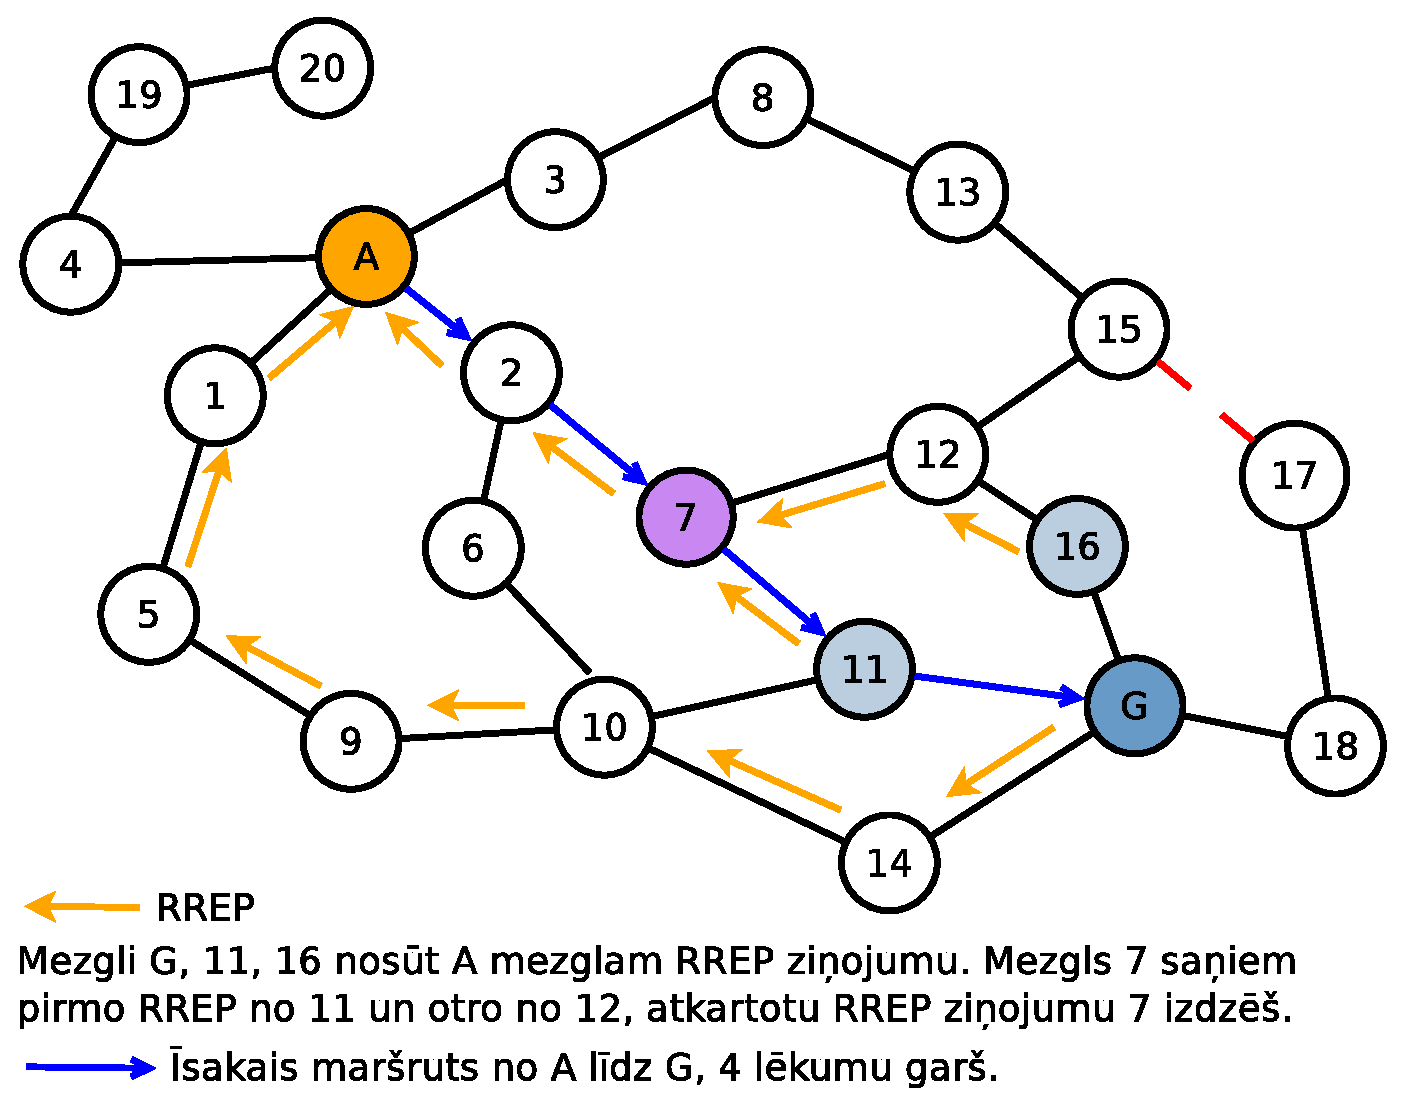
\includegraphics[scale=0.35]{./graph/aodv}
 \caption{AODV protokola datu pārraide tīklā}
\label{fig:aodv}
\end{figure}

Kad maršruts ir izveidots AODV izmanto to tik ilgi cik vien var. Savienojums var tikt izjaukts divu iemeslu dēļ: 1) ja neviens tam nesūta paketes un iestājas noilgums (time-out) un 2) ja kāds no mezgliem iziet no apraides. Ja aktīvi izmantots posms tiek pārtraukts, tad viens no kaimiņ-mezgliem nekavējoties izveido RERR ziņojumu. No maršrutēšanas tabulas mezgls izvēlās mezglus kam maršrutā paredzēts izmantot pārrautu posmu un nosūta tiem RERR. RERR ziņojums sastāv no ''DestCount'', nesasniedzamā galamērķa IP adreses, nesasniedzamā galamērķa kārtas (sequence) numura un galamērķa IP adreses. Kur ''DestCount'' skaits norāda cik galamērķi ir nesasniedzami, nesasniedzamā galamērķa kārtas (sequences) numurs ir kārtas numurs kas tiek ierakstīts mezgla maršrutēšanas tabulā.


AODV izmanto paplašinātu reģiona meklēšanas tehniku (expanding ring search technique), lai kontrolētu pārraides apgabalu. Faktiski, tas palielina dzīvošanas laika (TTL) ilgumu katrā RREQ pārraides kārtā līdz tam brīdim, kad tas saņems RREP. AODV, savukārt, strādā tikai ar simetriskām saitēm.

\subsubsection{AODV apkopojums}
Galvena AODV priekšrocība ir maršrutu izveidošana tikai pēc pieprasījuma. Tas ļauj būtiski samazināt periodisko kontroles ziņojumu virstēriņu, kas ir saistīts ar tabulas vadītu maršrutēšanu. Savukārt, kā trūkumu var minēt to, ka tiek radīta liela pārraides aizture kas ir saistīta ar jauna maršruta atklāšanu. Tas ir tāpēc, ka jaunu maršrutu meklēšanas laikā mezgls ienākošās paketes liek rindā, līdz tiek atrasts jaunais maršruts. Šis ir primārais aspekts, kas rada plūsmas kritumu izteikti mobilos tīklu gadījumos, jo dēļ mainīgas topoloģijas un relatīvi ilga  maršruta izveides laika liels pakešu skaits tiek vienkārši izmests.

\section{OLSR protokols}\label{sec:olsr}
\acf{OLSR} ir proaktīvs maršrutēšanas protokols, kas izveidots uz posma stāvokļa maršrutēšanas protokola bāzes. Klasiskā posma stāvokļa maršrutēšanas protokols  (LSRP) link state pakete satur visu kaimiņ-mezglu sarakstu un ar tiem asociētiem posma izmaksu metrika (link cost metric), kas izraisa lielu kontrolpaketes virstēriņu (overhead). Šis virstēriņš ir šķērslis šaurjoslas tīklos jo pakete tiek piegādāta katram tīklā esošam mezglam (pārpludināt). Padarot pārpludināšanas mehānismu efektīvāku un samazinot kontrolpaketes (contorl packet) virstēriņu jaunais protokols tika nodēvēts par optimizētu posma stāvokļa maršrutēšanas protokolu (\acs{OLSR}).

OLSR samazina atkārtoto pārraižu skaitu izmantojot vairākstāvokļu releju (\acs{MPR}). Tīklā tiek izvēlēti mezgli kas spēj viss efektīvāk pārklāt tīklu, tos dēvē par MPR mezgliem. MPR mezgli ir viena lēkuma (one-hop) kaimiņ-mezgli kuriem ir divvirzienu savienojums un viņi pēc kārtas pārklāj visus divu lēkumu kaimiņus (\figurename. ~\ref{fig:olsr}).

\begin{figure}[!htb]
\centering
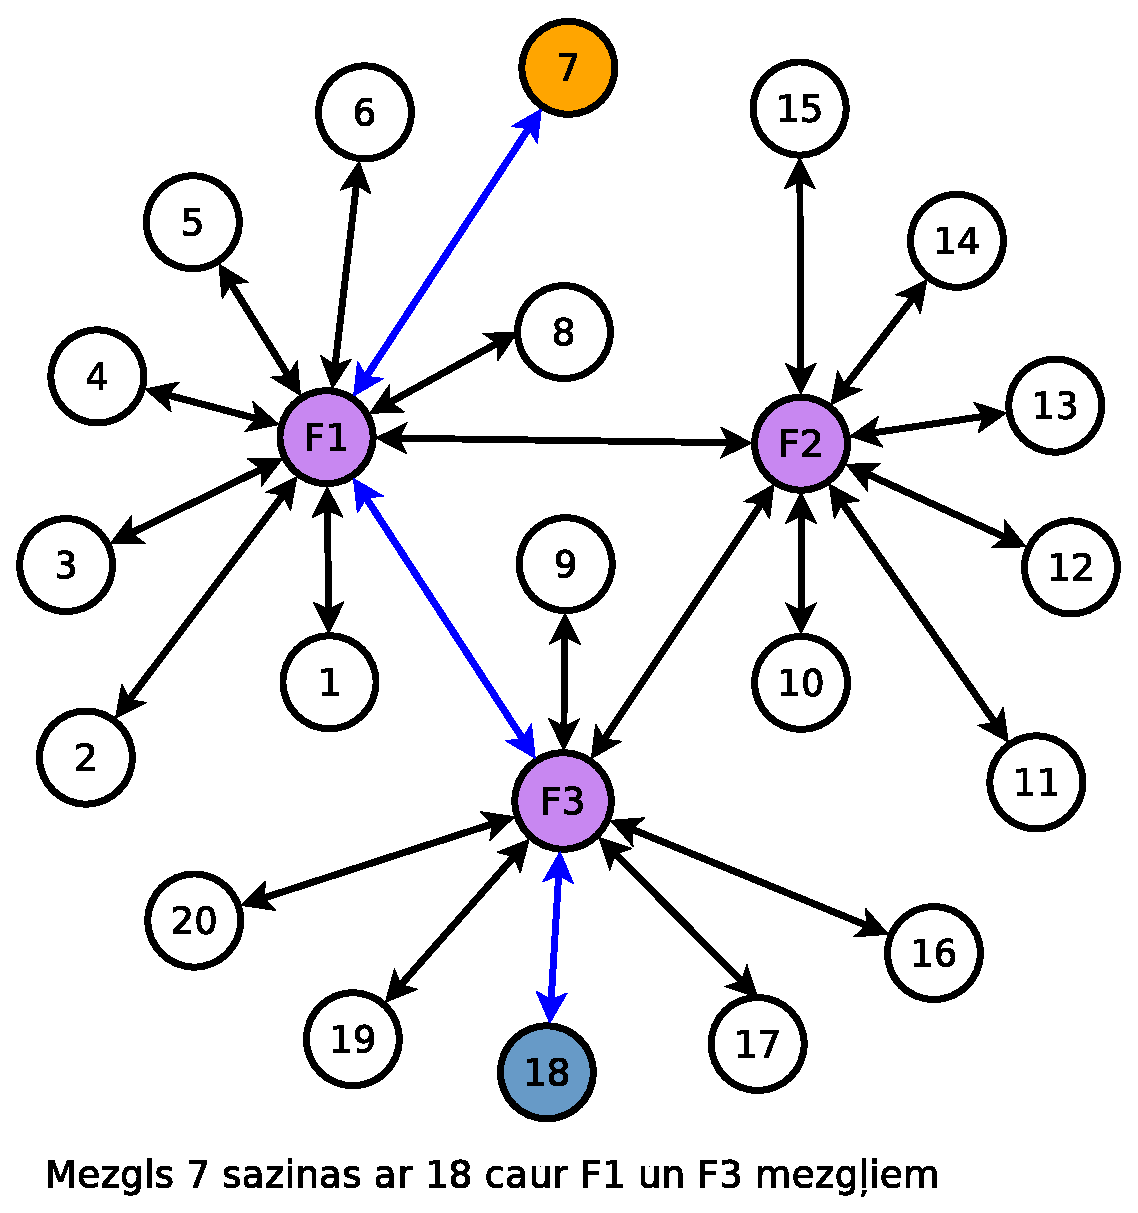
\includegraphics[scale=0.35]{./graph/olsr}
\caption{Datu pārraide tīklā ar OLSR protokolu}
\label{fig:olsr}
\end{figure}

Tīklā ar OLSR protokolu visi mezgli tiek iedalīti divās grupās: 1) MPRset (\figurename. ~\ref{fig:olsr} apzīmēti ar F1, F2, F3) un 2) MPRselctorset. Kur MPRset sastāv no izvēlētiem MPR mezgliem un MPRselectorset ir mezglu grupa, kuriem izvēlētais mezgls ir MPR mezgls. MPR mezgla izvēlētā grupa (MPRselectorset) darbojas kā pārsūtīšanas stacijas - tās saņem ienākošos datus un pārsūta tos uz galamērķi savā MPRselectorset. Šis paņēmiens palīdz samazināt virstēriņa posma statusa (link state) paketes, jo tikai MPR posma stāvokļa kontrolpaketē ir iekļauta posma stāvokļa statusā (link state connectivity) informācija.

Sākumā mezgli savu darbību uzsāk ar tukšām MPRset un MPRselectorset tabulām. Katrs mezgls izvēlas grupu no kaimiņ-mezgliem, tā lai katrs otrais kaimiņ-mezgls būtu sasniedzams ar šīs grupas starpniecību. OLSR izmanto vienkāršu zondēšanas shēmu lai atklātu kaimiņ-mezglu posma (link) statusu. Kaimiņmezglu posma statusam ir trīs iespējamās stadijas: vienvirziena (unidirectional), abu virzienu (bidirectional) un MPR. Periodiski OLSR izplata HELLO ziņojumu - šajā ziņojumā tiek iekļauti nesen komunicēto kaimiņ-mezglu saraksts un to posma statusi (link state). Kad mezgls saņem HELLO ziņojumu tas atzīmē posmu kā vienvirziena (unidirectional) lokālajā kaimiņ-mezglu tabulā un nākamajā HELLO ziņojumā iekļauj tajā sava kaimiņ-mezgla identifikatoru - ID. Kad kaimiņ-mezgls saņem šo HELLO ziņojumu ar savu ID tas atzīmē šo posmu kā abpusēju (bidirectional). Katrs mezgls izmanto dalītās aproksimācijas algoritmu (distributed approximation algorithm) lai izrēķinātu savu MPRset un marķē posmu ar šo mezglu kā MPR savā lokālajā tabulā.

RFC 3626  sadaļā 8.3.1, ir detalizēti aprakstīts heiristisks algoritms MPRset izrēķināšanai \cite{rfc3626}. HELLO ziņojumi tiek pārraidīti noteiktā MPRselctorset zonā, tādējādi samazinot joslas izmantošanu. No HELLO ziņojuma mezgli uzzina kas bija izvēlēts kā MPR mezgls. Saņemot HELLO ziņojumu MPR mezgls atzīmē sūtītāju savā MPRselectorset sarakstā. Visa tīkla posma statusa (link state) informācijas apmaņa notiek ar Topoloģijas uzraudzības ziņojumu (\acs{TC}). Periodiski katrs MPR mezgls tīklā pārraida pārējiem MPR mezgliem TC ziņojumu, kas satur MPR mezgla ID un tā MPRselectorset sarakstu. Šeit ir arī svarīgi atzīmēt, ka šādu ziņojumu sūta ne tikai tie MPR mezgli, kuriem MPRselectorset saraksts nav tukšs. Pamatojoties uz TC ziņojumu informāciju, mezgli var aprēķināt īsāko ceļu līdz katram mezglam tīklā. Ir svarīgi arī saprast, ka OLSR maršruts vienmēr iekļauj MPR mezglus kā retranslācijas punktu. Tāpēc OLSR maršruts nav iespējamais īsākais maršruts tīklā.

\subsubsection{OLSR apkopojums}
OLSR priekšrocība ir tā, ka šis protokols samazina kontroles informācijas apjomu un tādējādi izteikti samazina nepieciešamo trafika apjomu pārraidāmajā joslā. Lai arī OLSR iekļauj informāciju par katru maršruta posmu no avota līdz galamērķim, tas nebūt nenozīmē, ka piedāvātais maršruts ir visīsākais, jo notiek datu retranslācija caur MPR mezglu. Kā vēl vienu no OLSR protokola trūkumiem var minēt to, ka MPR mezglos, kad tie operē kā lokalizēti retranslējoši mezgli, ir novērojama maršrutēšanas aizture kā arī joslas virstēriņš. Tomēr, saskaņā ar protokola specifikāciju \cite{rfc3626}, OLSR uzrāda labus rezultātus ļoti blīvā tīklā ar augstu RWM mezglu kustību.

\section{Maršruta izvēles algoritma optimizācija}\label{sec:BERSP}
Šajā nodaļā apskatītie protokoli izmanto Bellman Ford algoritmu maršruta izvēlei, gadījumiem kad līdz vienam galamērķim ir pieejami vairāki maršruti. Izvēle tiek izdarīta vadoties pēc kopējā maršruta garuma, izvēloties visīsāko maršrutu (short-path). Īsākais maršruts nodrošina ātrāku datu pārraidi, bet tas ne vienmēr nozīmē arī visaugstāko servisa kvalitāti (QoS). \acl{QoS} tīklā ir atkarīga no bitu kļūdu intensitātes (\acs{BER}), datu pārraides ātruma un datu aizkavēm pārraides laikā. Ja maršrutēšanas protokols izvēlas maršrutu pēc Bellman Ford algoritma principa, tas, pirmkārt, mazina potenciālo datu aizkaves laiku un, otrkārt, saskaņā ar formulu (\ref{eq:BER_route}) (\seename \ref{sec:BER} sadaļu) mazinās $BER_{route}$, pie nosacījuma ka visos maršrutos $BER_{link}$ ir viens un tas pats. Taču jāņem vērā, ka mainīgas topoloģijas gadījumā šis nosacījumus nav iespējams.

Pēdējā laikā daži pētnieki piedāvā aizvietot Bellman-Ford algoritmu ar jauniem BER-bāzētiem algoritmiem \cite{olsr_ber} un \cite{qoS_static}.  T.Yelemou un P.Meseure savā darbā piedāvā BER-balstītu MPR izvēlētu OLSR maršrutēšanas protokolu \cite{olsr_ber}. Kā arī G.Ferrai un O.Tonguz \cite{qoS_static} piedāvā RESGO MAC BER-bāzētu protokolu, kas izvēlas maršrutu balstoties uz BER līmeni galamērķī. Tāds paņēmiens palīdz nodrošināt zemu BER līmeni, taču šis ieguvums, savukārt, tiek sasniegts ar maršruta garuma pieaugumu \cite{qoS_static}.

Abiem algoritmiem ir trūkumi un savas priekšrocības, lai mazinātu trūkumus šai maģistra darbā tiek  apskatīta iespēja apvienot šos algoritmus vienā algoritmā. Jaunais BER-SP algoritms ir balstīts uz kompromisu starp BER līmeni un posmu skaitu maršrutā. Tas izvēlas maršrutu ar īsāko maršrutu no saraksta kuram $BER_{route}$ ir zemāk par $BER_{app}$. Kur $BER_{app}$ ir BER līmenis kuru nepieciešams  nodrošināt pareizai lietojumprogrammas darbībai.  Algoritma darbība var tikt aprakstīta sekojošā veidā:
\begin{center}
 \begin{verbatim}
 1. Atrast visus zināmos maršrutus līdz galamērķim N
 2. Ja maršrutu skaits ir lielāk par 1, tad
     2.a No maršrutu saraksta izvēlēties vienu ar vissmazāko mezglu skaitu
     2.b Salidzīnāt izvēlētā maršruta BERroute ar BERapp
     2.c Ja  BERroute <= BERapp izvēleties šo maršrutu
     2.d Ja  BERroute > BERapp atkārtot procesu parējiem maršrutiem
 3. Ja otrajā solī netika izvelēts neviens maršruts
    3.a No saraksta izvēlēties maršrutu ar vismazāko BERroute
\end{verbatim}
\end{center}
Lai skaitliski pamatotu šī algoritma veiktspēju, izmantojot MATLAB tika simulēta SP, BER-bāzētu un BER-SP darbība izmantojot gadījuma lielumu $BER_{route}$ un $n_{h}$. Līdz vienam galamērķim ir 7 iespējami maršruti [$BER_{link}$ $n_{h}$], no šiem maršrutiem SP, BER-bāzēts vai SP-BER izvēlas vienu kas ''vislabāk'' atbilst algoritmu kritērijam. Programma izpilda 50 iterācijas lai izslēgtu nejaušības (MATLABa kodu skatīt \ref{appen:matlabSPBER}).

\begin{figure}
 \centering
 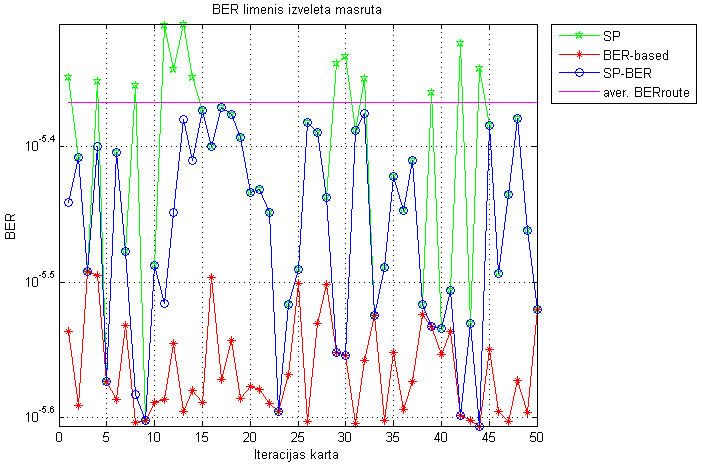
\includegraphics[scale=0.75]{./graph/BERSP_BER}
\caption{Dažādu algoritmu BER līmenis izēvelētajā maršrutā}
\label{fig:SPBER_ber}
\end{figure}

Attēlā \ref{fig:SPBER_ber} pāradīts BER līmenis izvēlētajā maršrutā atkarībā no maršrutēšanas algoritma. Uz Y ass izvietotas BER vērtības algoritmu izvēlētajā maršrutā un uz X ass iterācijas kārtas numurs. Salīdzinājumā ar SP algoritmu (attēlā zaļā krāsā) BER-SP (attēlā zilā krāsā) parāda labākus rezultātus, ko arī varējām gaidīt.
\begin{figure}[!htb]
 \centering
 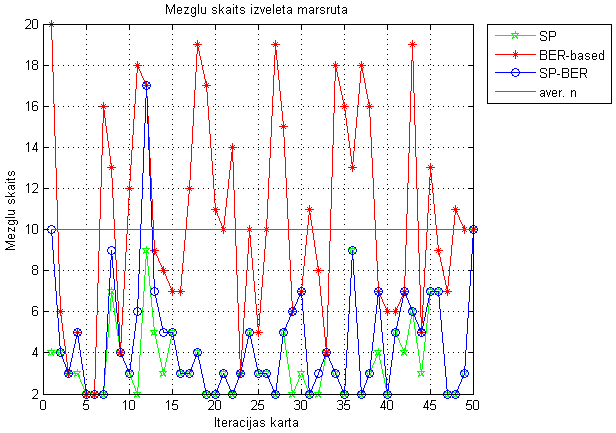
\includegraphics[scale=0.75]{./graph/BERSP_n}
\caption{Dažādu algoritmu posmu skaits izvēlētajā maršrutā}
\label{fig:SPBER_rho}
\end{figure}

Attēlā \ref{fig:SPBER_rho} pāradīts posmu skaits izvēlētajā maršrutā atkarībā no maršrutēšanas algoritma. Kā arī tika paredzēts, ka BER-bāzēta posmu skaits ir viss augstākais salīdzinājumā ar pārējo algoritmu izvēlētajiem maršrutiem. Savukārt BER-SP izvēlētajos maršrutos (attēlā zilā krāsā) vairākumā no posmu skaita kas ir mazāks par vidējo mezglu skaitu $n_{h}$(rozā līnija).

Šeit ir jāatzīmē, ka ir svarīgi noteikt pareizo $BER_{app}$ līmeni. Gadījumā kad $BER_{route}$ $\gg$ $BER_{app}$ BER-SP darbosies kā BER-bāzēts algoritms un izvēlēsies maršrutu ar viszemāko $BER_{route}$. Savukārt gadījumā, kad $BER_{route}$ $\ll$ $BER_{app}$ tas darbosies pēc SP algoritma principa, izvēloties visīsāko maršrutu jo visiem maršrutiem $BER_{route}$ ir zemāks par $BER_{app}$.

Maģistra dara izstrādes laikā nespēju atrast nevienu zinātnisku publikāciju, kas aprakstītu šādu maršrutēšanas algoritmu.
\chapter{Praktiskā daļa}\label{sec:prakt}
Šajā nodaļā, lai novērtētu mobilitātes ietekmi uz pakalpojuma kvalitāti bezvadu sensoru tīklos, aprēķiniem tiks izmantota lietojumprogramma MATLAB un \ac{NS-2} v.2-35. MATLAB ir izmantots BER līmeņa analīzei statiskā WSN tīkla kanālā, lai vēlāk šos datus saildzinātu ar NS-2 iegūtajiem rezultātiem.
Visās datorsimulācijās tika izmantoti tīkli ar vienādām fiziskā slāņa īpašībām. Pielikumā var apskatīt izmantoto NS-2 šablonu (\seename~\ref{appen:NETtempl}). Simulācijas parametri apkopoti Tab.\ref{tab:param}, maksimālā pārraides jauda un uztvērēja jūtīgums atbilst Lucent’s WaveLAN parametriem, tehnoloģija kuru iespējams pielietot WSN tīklu izveidei.
\begin{table}[!htb]
\centering
 \begin{tabular}{|l|c|c|}
\hline
~&\multicolumn{2}{c|}{Lucent’s WaveLAN}\\
\hline\hline
mezglu skaits&\multicolumn{2}{c|}{51}\\\hline
Tīkla laukums [$m\times m$]&1500$\times$300&500$\times$300\\\hline
Viļņu izplatīšanas veids&\multicolumn{2}{c|}{Two Ray Ground}\\\hline
Antenas veids&\multicolumn{2}{c|}{omnidirectional}\\\hline
Frekvence [MHz]& \multicolumn{2}{c|}{915}\\\hline
Raidītāja jauda [W]&\multicolumn{2}{c|}{0.001}\\\hline
Pārraides ātrums &2 [Mbit/s]&40 [Kbit/s]\\\hline
Radiouztvērēja slieksnis [W]&\multicolumn{2}{c|}{3.652$\times10^{-13}$}\\\hline
%Treshold to avoid collisions [W]&\multicolumn{2}{c|}{1.559x$10^{-11}$}\\\hline
Kolīziju slieksnis [dB]&\multicolumn{2}{c|}{10}\\\hline
MAC protokols& \multicolumn{2}{c|}{802.11}\\\hline
Traffika veids&\multicolumn{2}{c|}{CBR}\\\hline
Paketes garums [biti]&\multicolumn{2}{c|}{512}\\\hline
Pakešu izveides ātrums [pck/s]&\multicolumn{2}{c|}{4}\\\hline
Maršrutēšanas protokols&AODV&DSR\\\hline
Pakešu skaits rindā&\multicolumn{2}{c|}{64}\\\hline
Simulācijas laiks [s]&\multicolumn{2}{c|}{900}\\\hline
$t_{pause}$ [sek] &\multicolumn{2}{c|}{0, 30, 45, 60, 120, 300, 450, 600, 900}\\\hline
Komutācijas veids&\multicolumn{2}{c|}{NRBS}\\\hline
Mobilitātes Modelis&\multicolumn{2}{c|}{RWMM}\\\hline
$max$ mezglu ātrums [m/s]&\multicolumn{2}{c|}{0, 5, 10, 15, 20}\\
\hline
\end{tabular}
\caption{Simulācijas parametri}
\label{tab:param}
\end{table}

\section{Raiduztvērēju parametri}
Lai sasniegtu reālistiskos rezultātus tiek izmantoti reālo raiduztvērēju un raidītāju  parametri: Lucent’s WaveLAN frekvences ir $f_{c}$ = 915 MHz un raidītāj jauda $P_{t}$ ir 1mW.

\subsection{Radiouztvērēja slieksnis}
Ar radiouztvērēja slieksni $RXThresh\_$ raksturo minimālo jaudu kas ir nepieciešama veiksmīgai paketes saņemšanai. Lucent’s WaveLAN radiouztvērēja jutīgums ir -94 dBm, tātad $RXThresh\_$ = -94 dBm kas ir 3.981$\times10^{-13}$ W.\\
NS-2 vidē, ja pakete nonāk mezglā ar jaudu, kas ir lielāka vai vienāda ar slieksni, tad tiek uzskatīts, ka sūtītājs atrodas pārraides apgabalā un pakete ir veiksmīgi saņemta.

\section{MATLAB}
Mobilitātes apstākļos datu pārraidei ir nepieciešams nodrošināt divus nosacījumus: 1) mezgla A raidītājapgabalā ir jābūt uztvērēj-mezglam un 2) mezgliem jābūt vienam otra uztveršanas diapazonā  laika periodā $t$, lai pārraidītu $M$ garu ziņojumu pie datu pārraides ātruma $R_{b}$.

\subsection{Datu pārraides ātrums un mezglu kustības ātrums}
Savienojuma ilgumam jābūt tādam, lai laikā brīdi $t_{par}$ kaut vienu reizi nosūtīt ziņojumu uztvērēj-mezglam. Šo laika brīdi nosaka mezglu kustības ātrums un uztvērēj-mezgla jūtīgums, kā arī datu pārraides ātrums. Pie radiouztvērēja jutīguma -94 dBm, ideālos apstākļos kad interference netiek ņemta vērā, maksimālā distance pie kuras uztvērēj-mezgls saņems ziņojumu bez kļūdām  ir $r_{range}$ = 6.43 m (saskaņā ar (\ref{eq:r_range}) vienādojumu). Lai vienkāršot aprēķinus tiek pieņemts, ka divi mezgli kustas viens otram pretī ar vienādiem ātrumiem un sāk un pabeidz datu pārraidi $r_{range}$ attālumā no uztvērēj-mezgla (\seename ~\figurename. ~\ref{fig:mezgli}).

\begin{figure}[!htb]
\centering
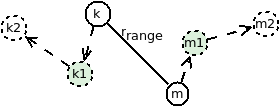
\includegraphics[scale=0.6]{./graph/mezgli.png}
\caption{Mezglu kustība}
\label{fig:mezgli}
\end{figure}

Tad laiks nepieciešams šķērsot šo attālumu pie mezglu vidējā ātruma no 5 līdz 20 [m/s] intervālā, būs vienāds ar

\begin{table}[!htb]
\centering
\begin{tabular}{|l|l|}
\hline
Vid. ātrums [m/s]&Laiks [s]\\\hline
5&1.286\\
10&0.643\\
15&0.428\\
20&0.321\\\hline
\end{tabular}
\caption{Laks lai šķērsot $r_{range}$ distanci pie dažādiem ātrumiem}\label{tab:atrumi}
\end{table}

Tagad zinot laika intervālu, var aprēķināt paketes skaitu ko mezgls nosutīs pie dažādiem datu pārraides ātrumiem.
\begin{figure}[!htb]
\centering
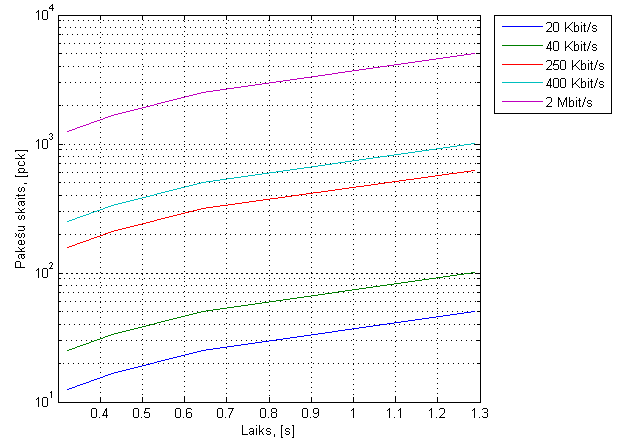
\includegraphics[scale=0.7]{./graph/vpck.png}
\caption{Pakešu skaits atkarība no datu pārraides ātrumiem}\label{fig:speed}
\end{figure}
Attēlā \ref{fig:speed} pieņemts ka paketes garums ir 512 biti, pakešu skaits būs atkarīgs no lietojumprogrammas. Lai iegūt pēc iespējas pilnīgu priekšstatu par tīkla darbību tiek pieņemts, ka datu pārraides ātrums ir 2 Mbit/s (augšēja robeža).

\subsection{Blīvuma ietekme}
Mezglu kustību var sadalīt relatīvi mazos laika posmos $\delta$t, tādos laika intervālos mobilo mezglu kustība būs tuva nullei (0). Un mobilo tīklu var apskatīt kā stacionāru. Izmantojot aprēķinu metodi (\seename ~\ref{sec:moby} sadaļu) tiek aprēķināta likumsakarība starp BER līmeni daudzposmu maršrutā un mezglu telpisko blīvumu tīklā. MATLAB programmu var apskatīt pielikumā (sk.~\ref{appen:matlabBERdensity})
\begin{figure}[!htb]
  \centering
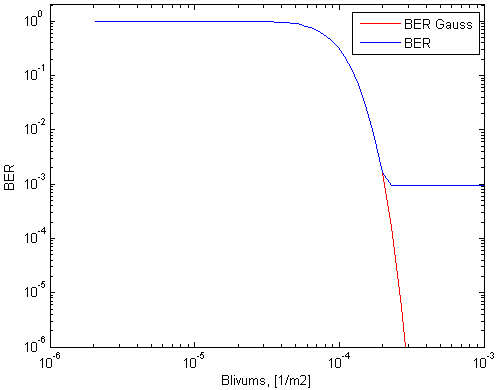
\includegraphics[scale=0.7]{./graph/blivBER.png}
\caption{BER daudzposmu maršrutā beigās atkarība no mezglu telpiska blīvuma tīklā}\label{fig:bliv}
\end{figure}

Attēlā \ref{fig:bliv} parādīta BER vērtībā atkarībā no mezglu izkliedes tīklā, kur sarkanā līnija ir $BER_{Gauss}$, kas ir aprakstīta šī darba \ref{sec:moby} sadaļā un zilā atbilst G.Ferrati un O.Tonguz piedāvātai metodei \cite{qoS_mobility} kurā, kad $\rho\rightarrow\infty$  tad $BER_{link} \simeq \frac{3\lambda M}{4R_{b}}$. Un $BER_{route}$ būs
\begin{equation}
 BER_{route}\simeq max \left \{  \left[ 1- \left[1-Q\left(\sqrt {\frac{2Pr}{Ptherm+Pini}}\right)\right]^{n_{h}}\right], \frac{3n_{h}\lambda M}{4R_{b}}\right \},
\end{equation}
kur $M$ ir ziņojuma garums.

Kā jau iepriekš tika minēts - lai izveidotu savienojumu ir nepieciešams uztvērēj-mezgls raidīšanas diapazonā laika periodā $t_{par}$. Pie zema $\rho_{s}$ BER līmenis daudzposmu maršruta beigās ir gandrīz viens (1), tādēļ tā raidītā jauda ir nepietiekami augsta lai pārraidītu signālu tik lielā attālumā. Savukārt pie $\rho_{s}$ ap  $5\times10^{-4}$ tas pazeminās, šajā robežā uztvērēj-mezgla jutīgums ir pietiekami augsts lai uztvert signālu, turklāt interference no apkārt esošiem mezgliem ir niecīga. Savukārt ar $r_{link}$ ($r_{link}=1/\sqrt{\rho_{s}}$) pazemināšanu kanālā palielinās interferences un tas ir galvenais trokšņu avots.
Ņemot vērā iepriekš teikto šajā darbā NS-2 realizētajos scenārijos būs apskatīts tīkls ar telpisko blīvumu $\sim10^{-4}$ lai izslēgtu varbūtību, ka datu pārraide tiek traucēta kāda cita iemesla dēļ.


\section{NS-2 simulācijas}
\acf{NS-2} lietojumprogramma ir diskrēto notikumu modelējoša (discrete event simulator) programma, kas bieži tiek izmantota telekomunikāciju tīklu pētījumos. Ar NS-2 iespējams modelēt TCP, maršrutēšanas un multiraides protokolu darbību vadu un bezvadu (WLAN, WPAN un satelīt) tīklos \cite{ns2}.

Maģistra darbā izmantoto NS-2 simulāciju scenāriju pilns apkopojums ir iekļauts maģistra darbam pievienotajā CD - ''Maģistra darbā ''Mobilitātes ietekme uz pakalpojuma kvalitāti sensoru tīklos'' izstrādātie NS-2 simulāciju scenāriji''.


\subsection{Datorsimulācijas parametri}

\subsubsection{Kolīziju slieksnis}
Datu pārraides laikā var gadīties, ka galamērķī vienlaicīgi pienāk divas paketes, izraisot kolīziju. NS-2 vidē kolīziju potenciāli var izraisīt tikai paketes ar jaudu, kas ir augstāka par $RXThresh\_$. Ja abām paketēm jaudas ir augstākas par $RXThresh\_$, tad to jaudu attiecības tiek salīdzinātas ar kolīziju slieksni $CPThresh\_$. Šajā eksperimentā kolīziju slieksnis tiek pieņemts $CPThresh\_$ = 10 dB.

\subsubsection{Viļņu izplatīšanās veids}
Tiek uzskatīts, ka tīkls ir plakana virsma un visi mezgli kustās tikai X un Y koordinātēs. Līdz ar to, lai sasniegtu iespējami reālistiskus rezultātus, tiks izmantots ''two-ray ground'' modelis. Šajā modelī uztvertā jauda tiek raksturota ar Friis formulu (\seename (~\ref{eq:pr}) formulu) ar $\gamma$ = 4.  Two-ray ground modelī mezgls uztver gan atstaroto signālu gan arī to, kas nonāk līdz mezglam bez atstarojuma. Lai izmantotu šo modeli NS-2 mezglu antenām ir jābūt izvietotām vienādā augstumā, tāpēc visos scenārijos tiek pieņemts, ka Z = 1.5 m.

\subsubsection{MAC protokol}
IEEE 802.11 standartā, RREQ paketes tiek pārraidītas apraides (broadcast) veidā, savukārt RREP un RERR un  datu pakešu pārraide notiek uniraides  veidā, šāda tipa paketes ir adresētas noteiktiem kaimiņ-mezgliem. Savienojuma pārrāvums tiek konstatēts ar MAC līmeņa palīdzību. Kad MAC līmenis uniraides paketes posmā otram mezglam vairs nespēj piegādāt paketes, tad uz maršrutēšanas līmeni tiek nosūtīts signālziņojums. Piemēram, gadījumos kad pēc datu pārraides beigām netiek saņemta ACK pakete.

\subsubsection{Buferis}
Visi šajā nodaļā apskatītie maršrutēšanas protokoli uztur nosūtīšanas buferi, kura garums ir 64 paketes. Paketes, kurām maršruta atklāšanas (route discovery) process ir ticis iniciēts, taču mezglā vēl nav saņemta RREP pakete, tiek ievietotas buferī. Gadījumā, kad pakete atrodas buferī ilgāk par 30 sek. tā tiek dzēsta. Līdz mirklim kad MAC līmenis atkal būs pieejams gan datu, gan maršrutēšanas paketes tiek ievietotas rindas interfeisā (interface queue). Rindas interfeisa garums ir 64 paketes un tajā maršrutēšanas protokoliem ir prioritāte, visas parējās paketes tiek sūtītas rindas kartībā.

\subsubsection{Trafiks un Mobilitātes modelis}
Šajā simulācijā tika izmantots konstants bitu ātruma (\acs{CBR}) avots, ar konstantu pakešu izveides ātrumu $\lambda$ [pck/s]. Avots-galamērķis pāris ir nejauši izvietots tīkla laukumā. NS-2 standart pakā ir iebūvēta \texttt{cbrgen.tcl} utilītprogramma trafika automātiskai izveidei. Ar šo utilītprogrammu tika izveidoti CBR trafika šabloni, kas savukārt turpmākajā darbā tika izmantoti kā ievaddati. Visās simulācijas mezglu mobilitātei ir izmantots (\acs{RWMM}) (\seename nodaļa ~\ref{sec:mobilityModels}). \acf{RWMM} mezgli kustas ar gadījuma ātrumu [$v_{min}, v_{max}$] līdz gadījuma mērķim. Simulācijas mērķis bija noteikt mezglu mobilitātes ietekmi uz QoS pie dažādiem ātrumiem. Visu simulāciju ilgums ir 900 sek. un simulācijas sakumā katrs mezgls ir nekustīgs $t_{pause}$ laika periodu.
Pauzes laiks $t_{pause} = 0$ atbilst nepārtrauktai mezglu kustībai (saskaņā ar RWMM modeli), savukārt $t_{pause} = 900$ sek. atbilst stacionāram tīklam kurā kustības nav, jo pauze ilgst visu simulāciju. RWMM kustības šablona izveidošanai tika izmantota NS-2 iebūvētā utilītprogramma \texttt{setdest.tcl}.

\subsubsection{Enerģija modelis}
Enerģijas modelis ir iebūvēts NS-2 kā mezglu atribūts. Enerģijas modelī ir ''initial value'' kas atbilst enerģijas līmenim darbības sakumā un pēc katras paketes pārraides/saņemšanas tas ņem vērā ar to saistīto enerģijas patēriņu. Kad mezgla enerģijas līmenis sasniedz nulli, mezgls ''nomirst'', tas vairs nevar saņemt, retranslēt vai nosūtīt paketes. Šajā darbā enerģijas patēriņš netiek ņemts vērā.


\subsection{Veiktspējas analīzes parametri}
Šajā darbā tiek pētīta mobilitātes ietekme uz servisa kvalitāti WSN tīklā. QoS līmenis ir noteikta prasību kopa kuru tīklam ir jānodrošina pārraidot datus no avota līdz galamērķim. Mobilitātes un dinamiskās topoloģijas dēļ, kā arī dēļ fiziskā slāņa ierobežojumiem var gadīties, ka tīkla resursi ne vienmēr ir pieejami pilnā apjomā visu pakešu vienlaicīgai pārraidīšanai. Līdz ar to, tādi parametri kā, piemēram, caurlaidspēja, aizkavē pakešu izmešanu (packet drop) un tam ir jāpievērš pastiprināta uzmanība. Lai noteiktu pakalpojumu kvalitāti stacionārā un mobilā WSN tīklā, tika izmantoti sekojoši veiktspējas parametri. \ac{PDF} un vidējā aizkave tīklā ir vieni no svarīgākajiem parametriem veiktspējas analīzē.

\subsubsection{\acl{PDF}}
\acf{PDF} ir attiecība starp veiksmīgi saņemtām CBR paketēm un summu visu izveidoto CBR pakešu simulācijas laikā. Tas ir svarīgs parametrs kas norāda uz tīkla pārblīvi\footnote{Pārmērīgi intensīva ziņojumu plūsmu, kas aizkavē ziņojumu pārsūtīšanu datoru tīklā, nelabvēlīgi ietekmē datoru tīkla veiktspēju un var radīt pārraidāmās informācijas zudumus \cite{lza}.} tīklā. PDF palīdz raksturot protokola veiktspēju vadoties pēc pakešu pazaudēšanas koeficienta (packet loss rate), ko ietekmē tādi faktori kā paketes garums, tīkla noslodze un mainīga topoloģija. Augsts PDF lielums nozīmē, ka pazaudētu pakešu skaits ir zems un no datu nosūtīšanas viedokļa protokols ir efektīvs. Šeit ir svarīgi atzīmēt, ka pie augsta PDF pakete, kas saņemta ar lielu aizkaves laiku ir nederīga. PDF un laika aizkave ir vienādi svarīgi parametri.
\begin{equation}
 PDF=\frac{\sum Sa_{CBR}}{\sum No_{CBR}},
\end{equation}
kur $Sa_{CBR}$ ir visās veiksmīgi saņemtas CBR paketes un $No_{CBR}$ ir visas nosūtītās CBR paketes.

\subsubsection{Vidēja aizkavē tīklā}
Vidējā aizkave tīklā, jeb abpusējā aizkave (end-to-end delay), ir vidējā laika starpība starp laika brīdi kurā paketi tika izveidota avotā, līdz brīdim kad tā tika saņemta galamērķī. Pazaudētās paketes netiek ņemtas vērā. Savukārt, tiek ņemtas vērā aizkaves kas ir radušās dēļ maršruta atklāšanas (route discovery), atkārtotām pārraidēm,  gaidīšanas laika rindā un viļņu izplatīšanās laiks. Visu savienojumu aizkaves tiek summētas kopā un tiek dalītas ar izveidoto savienojumu skaitu visas simulācijas laikā.
\begin{equation}
Avg.delay=\frac{\sum( Laiks_{gal} - Laiks_{avots})}{\sum N_{sav}},
\end{equation}
kur $Laiks_{gal}$ ir laika brīdis kurā pakete nonāk galamērķī, $Laiks_{avots}$ ir laika brīdis, kurā avots izsūtīja šo paketi un $N_{sav}$ ir savienojumu pāru skaits tīklā.

\subsubsection{Caurlaidspēja}
Tīkla caurlaidspēja ir datu daudzums kas vienas sekundes laikā tiek pārraidīts no avota uz galamērķi. Analizējot iegūtos datus tika ņemtas vērā tikai CBR paketes, ignorējot papildus tēriņus - tādus kā HELLO, RREQ un RREP utt.. Tika aprēķinātas divas caurlaidspējas: 1) mezgla caurlaidspēja - attiecība starp mezglā veiksmīgi saņemtu pakešu skaitu pret kopējo bitu skaitu simulācijas laikā. 2) Tīkla caurlaidspēja, kas ir vidējā mezglu caurlaidspēja tīklā - skaitot tikai tos mezglus, kas ir iesaistīti CBR datu pārraidē.
\begin{equation}
 n_{through}=\frac{\sum n_{bit}}{t_{sim}},
\end{equation}
kur $\sum n_{bit}$ ir summārais mezglā saņemto bitu skaits un $t_{sim}$ ir simulācija ilgums.
\begin{equation}
Tīkla.caurlaidspēja =\frac{\sum n_{through}}{N},
\end{equation}
kur $ \sum n_{through}$ ir visu mezglu summārā caurlaidspēja un $N$ ir  kopējais mezglu skaits tīklā.


\section{Rezultātu analīzē}
Simulācijas laikā iegūte rezultāti raksturo procesus tīklā ar telpisko blīvumu $\rho_{s} = 1.13\times10^{-4}$, distance starp raidītājmezglu līdz uztvērējmezglu ir $r_{link} = 134.2$ m un 10 no 51 mezgla ģenerē datus. Lai visi simulāciju scenāriju būt pēc iespējas vienādi, stacionārā tīkla mezglu izvietojums tika izveidots pēc tā pāša principa kā pārējie, ar tādu atšķirību, ka mezglu ātrums vienāds ar 0.01 [m/s] un pauzes laiks vienāds ar 900 sekundēm.

\subsection{Paketes piegādes sadale un vidējā aizkava tīklā}
\begin{figure}[htb!]
\begin{minipage}[t]{0.47\linewidth}
\centering
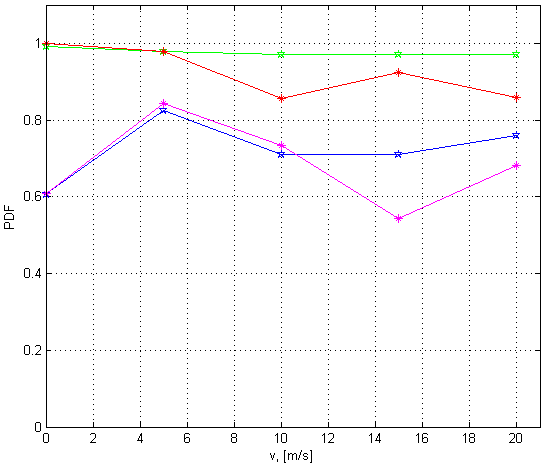
\includegraphics[scale=0.55]{./graph/vPDF.png}
\caption{Paketes piegādes sadales atkarība no maksimālā ātruma}
\label{fig:pdfspeed}
\end{minipage}%
\hspace{0.2cm}
\begin{minipage}[t]{0.47\linewidth}
\centering
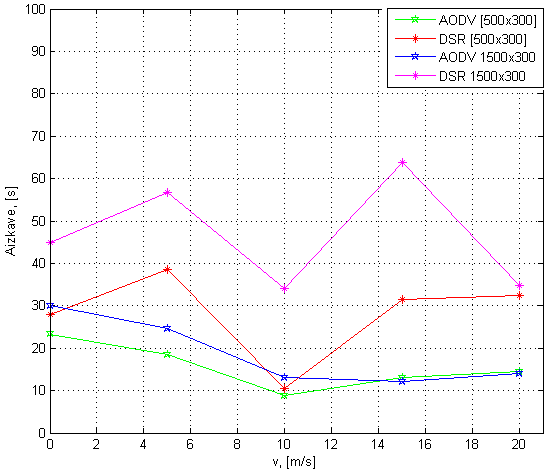
\includegraphics[scale=0.55]{./graph/vDelay.png}
\caption{Vidējā aizkave tīklā atkarībā no maksimālā ātruma}
\label{fig:avgDspeed}
\end{minipage}
\end{figure}
Attēlā \ref{fig:pdfspeed} parādīta PDF atkarība no maksimālā mezglu ātruma ar AODV un DSR maršrutē-šanas protokoliem, un tīkla telpiskā blīvuma $\rho_{1500\times300}$ = 1.13$\times10^{-4}$ un $\rho_{500\times300}$ = 3.4$\times10^{-4}$, [$\frac{1}{m^{2}}$]. Pie $\rho_{500\times300}$ = 3.4$\times10^{-4}$ stacionārā tīklā PDF ir gandrīz vienāds ar 1. Ar kustības sākumu tas degradē, it sevišķu gadījumos, kad tiek pielietots DSR protokols, pie maksimālā ātruma 20 [m/s] tas tuvinās pie 0.8 (datu piegāde krīt par $\sim$17\%). Savukārt pie $\rho_{1500\times300}$ = 1.13$\times10^{-4}$ stacionāram tīklam PDF ir vienāds tikai ar 0.6 un mezglu mobilitātes apstākļos tā pieaug vidēji par $\sim$12\%, sasniedzot maksimumu pie ātruma 5 [m/s]. PDF pārsniedz 0.8.

Kā var redzēt attēlā \ref{fig:pdfspeed} maršrutēšanas protokola izvēle lielā mērā ietekmē kopējo tīkla veiktspēju mobilitātes apstākļos. Ar mezglu ātrumu pieaugumu DSR protokols uzrāda aizvien sliktākus rezultātus salīdzinājumā ar AODV. Tas ir izskaidrojams ar to ka DSR protokols ir distances vektora protokols un mezgls savā kešatmiņā uztur datus tikai par maršrutiem līdz 1. kārtas kaimiņ-mezgliem. Jo straujāk mainās topoloģija (šajā gadījumā jo ātrāk kustas mezgli) jo vairāk DSR maršrutēšanas pakešu nepieciešams lai izveidotu datu pārraidi.

Daudzas lietojumprogrammas piegādātās paketes ar lielu laika aizkavi tiek uzskatītas per nederīgām. Attēls \ref{fig:avgDspeed} ilustrē tīkla vidējās aizkaves izmaiņas atkarībā no mezglu maksimālā kustības ātruma. Viszemākā aizkave tīkla ir pie maksimālā ātruma 10 [m/s]. Tas nozīmē, ka pie mezglu maksimālā kustības ātruma 10 [m/s] (vidēja 7.5 [m/s], no \texttt{trace} failā). Salīdzinājumā ar statisko tīklu pie $\rho_{500\times300}$ = 3.4$\times10^{-4}$ mobilitāte ļauj samazināt vidējo pakešu aizkavi pat 2 reizes. Savukārt AODV atkal uzrāda labākus rezultātus salīdzinājumā ar DSR. Mobilitātes apstākļos AODV spēj nodrošināt datu maršrutēšanu ar vidējo aizkavi tīklā ne augstāku par 15 sekundēm (kad mezglu maksimālais ātrums pārsniedz 5 [m/s]). Tas ir saistīts ar to ka informācija par tīkla topoloģiju izplatās daudz ātrāk nekā stacionārā.

\subsection{Caurlaidspēja}
\begin{figure}[!htb]
\centering
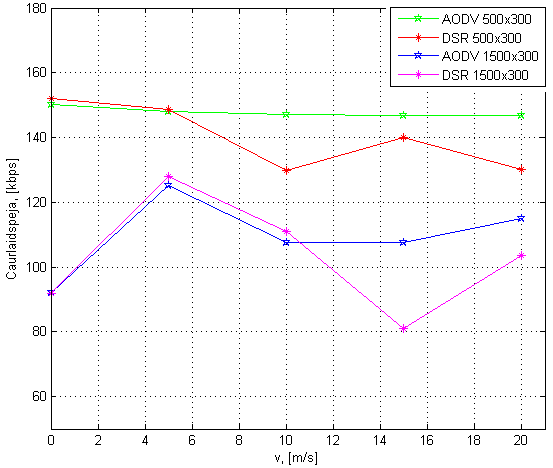
\includegraphics[scale=0.75]{./graph/vThrough.png}
\caption{Tīkla vidēja caurlaidspēja atkarība no maksimālā ātruma}
\label{fig:avgT}
\end{figure}
Kā var redzēt attēla  \ref{fig:avgT} pie mezglu telpiskā blīvuma 3.4$\times10^{-4}$ tīkla vidējā caurlaidspēja samazinās un tam ir loģisks izskaidrojums - pieaug maršrutēšanas pakešu skaits, kas ir nepieciešams datu pārraides izveidošanai. Savukārt, pie $\rho_{1500\times300}$ = 1.13$\times10^{-4}$ tīkla vidēja caurlaidspēja pieaug salīdzinājumā ar tā paša tīkla statisko modeli. Līdz ar to ir iespējami divi izskaidrojami, pirmkārt datu pārraide pieaug tādēļ ka kustīgi mezgli spēj ātrāk piegādāt datus līdz galamērķim. Gadījumā kad mezgli ir izkliedēti tīkla, mezglu kustība ļauj ātrāk pārvietot informāciju telpā, neatkarīgi no maršrutēšanas protokola. Savukārt pie 3.4$\times10^{-4}$ mobilitāte traucē it sevišķi DSR protokola izmantošanas gadījumā.

Ņemot vērā mezglu izkliedes pakāpi, vislabākos rezultātus uzrād AODV protokols pie $\rho_{1500\times300}$ = 1.13$\times10^{-4}$ vidēji paaugstinot tīkla caurlaidspēju par 15 [Kbit/s], kas ir aptuveni 18\% no stacionārā tīkla.

\subsection{AODV protokola veiktspēju atkarība no pauzes laika}
Iepriekšējā sadaļā bija apskatīta AODV un DSR protokolu darbība tīklā  ar nepārtraukti kustošiem mezgliem. Savukārt, ja gribam iegūt labāku priekšstatu par mobilitātes ietekmi uz tīkla darbību, tad ir nepieciešams novērtēt kustības maiņas ietekie. Gadījuma maršrutpunktu mobilitātes modelī mezgls sasniedzot savu galamērķi var uztaisīt pauzi uz kādu  $t_{pause}$ laiku, šajā laikā brīdi mezgla ātrums $v$ vienāds ar 0. Pēc pauzes mezglam tiek piešķirts jauns ātrums un jauns galamērķis. Lai uzzinātu kā AODV protokols spēj darboties pie dažādām mobilitātes pakāpēm, $t_{pause}$ tiek piešķirti sekojošas vērtības [0, 30, 45, 60, 120, 300, 450, 600, 900] sekundes un ar $\rho_{1500\times300}$ = 1.13$\times10^{-4}$.

\begin{figure}[htb!]
\begin{minipage}[t]{0.47\linewidth}
\centering
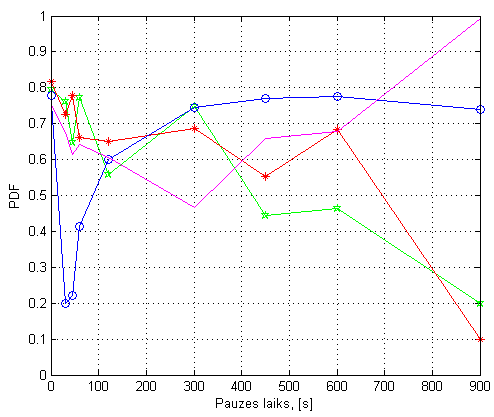
\includegraphics[scale=0.55]{./graph/pdf.png}
%\caption{Paketes piegādes sadale atkarība no pauzes laika}
%\label{fig:pdf}
\end{minipage}%
\hspace{0.2cm}
\begin{minipage}[t]{0.47\linewidth}
\centering
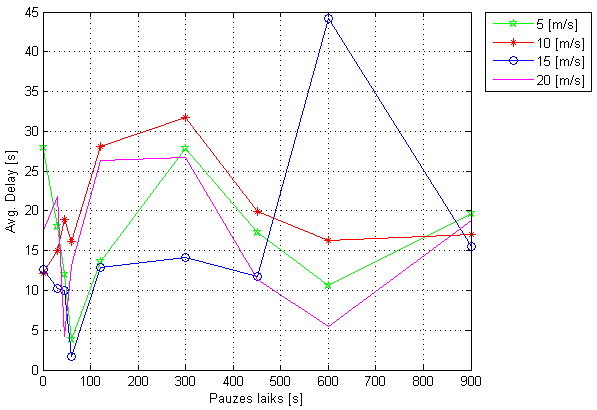
\includegraphics[scale=0.55]{./graph/avgD.png}
%\label{fig:avgD}
\end{minipage}
\caption{Vidēja aizkavē tīklā atkarība no pauzes garuma}\label{fig:pause}
\end{figure}
Attēlā \ref{fig:pause} pāradīta AODV protokola veiktspēja kā funkcija no pauzes garuma. Pie augstas mobilitātes, kad $t_{pause}$ ir zemāka par 300 sekundēm, salīdzinājumā ar $t_{pause}$ = 0 notiek aptuveni 15\% PDF kritums, savukārt, vidējā aizkave samazinās divas reizes pie $t_{pause}$ [30 - 120] sek. No kā var secināt, ka pauzes intervāls 60 sekundes (aizkavē mazāk nekā 5 sekundes) ir laiks kas ir nepieciešams AODV lai pielāgotu maršrutu. Par jebkurām izmaņām maršrutā ir jāmaksā ar datu pārraides daudzumu un pie $t_{break}$ = 60 PDF samazinās par 10\%. AODV maršrutēšanas paketēm ir prioritāte rindā. Šeit ir svarīgi atzīmēt ka, scenārijā pakešu garums ir 512 biti un tie ražoti ar ātrumu 4 pck/s, kas kopumā rāda augstu tīkla noslodzi. Kā arī mezglu izvietojums tīkla laukumā, koordinātēs X un Y ir gadījuma lielumi, un būtiski ietekmē datu pārraidi pie tik zema telpiskā blīvuma (1.13$\times10^{-4}$, [$\frac{1}{m^{2}}$]). Kā piemēram, att. \ref{fig:pause} vidējā aizkavē pie ātruma 15 [m/s] pārsniedz 40 sekundes. Šī darba mērķis ir iegūt vispārējo priekšstatu par mobilitātes ietekmi, lai iegūt likumsakarības starp pauzes laiku un protokola veiktspēju ir nepieciešams atkārtot aprakstīto scenārijus vairākas reizes un no iegūtajiem rezultātiem aprēķināt vidējo vērtību.
\chapter{Secinājumi}\label{sec:secin}
% raksturo materiālu (datu) vākšanā un analīzē pielietoto pētniecisko metodi, apkopo maģistra darba argumentāciju un teorētiskos un praktiskos secinājumus.
% Darba nobeigumā autors lakoniski definē secinājumus, darba rezultātus un iespējamās rekomendācijas. Pēc maģistra darba teksta, seko secinājumi (tēzes) īsā, lakoniskā veidā, rindkopu formā. Tās numerācijas secībā
%3. izvēlētās pētniecības metodes un objektus
Tuvāk iepazīstoties ar mobiliem bezvadu sensoru tīkliem (WSN) kļūst skaidrs, ka tīkla veiktspēja un servisa kvalitāte (QoS) tajā ir atkarīgi no daudziem faktoriem. Kuru starpā vissvarīgākie ir mobilitāte, mezglu telpiskais blīvums un maršrutēšanas protokola veiktspēja. Pārsvarā mobilie WSN tīkli tiek pētīti pie ideāliem apstākļiem izdalot tājos vienu vienīgu pētāmo parametru. Šajā darbā tika izmantota semi-analītiskā pieeja lai pētītu saistības starp mezglu mobilitāti, maršrutēšanas protokolu un fiziskā slāņa īpašību ietekmi uz QoS līmeni daudzposmu maršrutā.

Bezvadu sensoru tīkli ir diezgan jauna tehnoloģija, un līdz ar to trūkst reālo datu par tajā notiekošiem procesiem, kā arī pētīšanas process tiek apgrūtināts ar ļoti plašu pielietošanas spektru. Pēc šī darba izstrādes viennozīmīgi varu apgalvot, ka lai nodrošinātu pētniecisku progresu šinī nozarē ir nepieciešams: 1) izveidot pamatnostādnes un ierobežot pielietošanas apgabalu 2) būvēt un  pētīt reālus tīklus, nevis balstīt pētījumus tikai uz datorsimulācijas rezultātiem. Nodaļā \ref{sec:tris} apkopoti teorētiskie aspekti var tikt pielietoti, kā sākum pozīcija WSN fiziskā slāņa parametru aprēķiniem.

Darba gaitā tika piedāvāta maršruta izvēles algoritma optimizācija (\seename ~\ref{sec:BERSP} sadaļu), piedāvātais algoritms ir kompromiss starp BER līmeni un posmu skaitu maršrutā. Tas izvēlas maršrutu ar vismazāko posmu skaitu no iespējamiem maršrutiem kuros $BER_{route}$ ir zemāks par $BER_{app}$. Kur  $BER_{app}$ līmeni nosāka lietojumprogramma vai tīklā administrators. Gadījumā, kad visu iespējamo maršrutu līmenis $BER_{route}$ ir augstāks par $BER_{app}$ BER-SP algoritms darbosies, kā BER-bāzēts algoritms un izvēlēsies maršrutu ar viszemāko $BER_{route}$. Un gadījumā, kad pieejamu maršrutu $BER_{route}$ ir zemāks par $BER_{app}$, BER-SP algoritms darbosies pēc SP algoritma principā, izvēloties visīsāko maršrutu jo visiem maršrutiem $BER_{route}$ ir zemāk par $BER_{app}$. Ar nelielu simulāciju MATLABā (\seename ~\figurename. ~\ref{fig:SPBER_ber}) tika pierādīts ka šim paņēmienam ir acīmredzama priekšrocība salīdzinājumā ar īsākā ceļa (short-path) un BER-bāzes algoritmu. Lai pilnībā novērtētu šo algoritmu ir nepieciešami papildus pētījumi NS-2 vidē.

Attēlā \ref{fig:bliv} parādīta likumsakarība starp BER līmeni daudzposmu maršrutā un mezglu telpisko blīvumu tīklā. Pie mezglu telpiskā blīvuma zemāk par $5\times10^{-4}$ BER līmenis daudzposmu maršruta beigās sasniedz 1. Kas ir izskaidrojams ar pārāk lielu distanci starp raidītāju un uztvērēju. Ja aprēķiniem tiek izmantot AWGN kanāls tad BER no $5\times10^{-4}$ tas strauji tiecas uz 0. Kas neatbilst reālajai situācijai, jo tuvāk ir raidošie mezgli jo augstāka ir mezglu savstarpējā interference. Gadījumā kad datu pārraide tīklā tiek ietekmēta ar augstu interferenci, maršrutēšanas protokols nevar pozitīvi ietekmēt tīkla veiktspēju \cite{qoS_mobility}. Līdz ar to NS-2 simulācijai tika izvēlēti divi telpiski blīvumi $\rho_{1500\times300} = 1.13\times10^{-4}$ un $\rho_{500\times300} = 3.4\times10^{-4}$, [$\frac{1}{m^{2}}$].

Pēc darba izstrādes ir grūti viennozīmīgi pateikt vai mobilitātei ir pozitīvā vai negatīva ietekme, jo tas, ko esmu konstatējusi ar veiktajām simulācijām un aprēķiniem  ir tas, ka ir jāpēta parametru kombinācijas: mezglu kustības ātrums, telpiskais blīvums, datu pārraides ātrums un izmantotais pakešu garums. Kā arī mobilitātes modelim ir ļoti liela ietekme uz rezultātiem. Attēlā ~\ref{fig:pause} ir pāradīti rezultāti AODV protokola veiktspēja pie RWMM dažādiem pauzes garumiem. Kad pauzes laiks ir intervālā no 30 līdz 120 AODV protokolā veiktspēja pasliktinās par ~10\% salīdzinājumā kad tas ir 0. Tas ir jāņem vērā novērtējot mobilitāti. Taču nav iespējams aprēķināt visas parametru kombinācijas un to lielumu variācijas. Tātad, var secināt, ka ir svarīgi zināt sistēmas prasības, lai varētu noteikt mobilitātes ietekmi.

Šai darbā izvēlētajai sistēmai (\seename \ref{sec:petPar} sadaļu) pie maksimāljiem mezglu kustības ātrumiem 5 un 10 [m/s] un izmantojot AODV maršrutēšanas protokolu mobilitātes ietekme ir bijusi pozitīva. \acf{PDF} (\seename ~\figurename~\ref{fig:pdfspeed}) sasniedz 0.8 un ir novērojama viszemākā vidējā pakešu aizkave < 10 sek. (\seename ~\figurename ~\ref{fig:avgDspeed}) un tīkla caurlaidspēja pārsniedz 120 [Kbit/s] (\seename ~\figurename ~\ref{fig:avgT}). Balstoties uz iegūtiem rezultātiem, var viennozīmīgi apgalvot, ka AODV protokola veiktspēja, it sevišķi pie zemā telpiska blīvuma, ir daudz labāk nekā DSR (\seename ~\figurename ~\ref{fig:avgDspeed}, ~\ref{fig:pdfspeed}, ~\ref{fig:avgT}). AODV spēj ātrāk pielāgot maršrutu manīgas topoloģijas apstākļos ar mazāku ietekmi uz caurlaidspēju.

Vēl jāpiemin, ka NS-2 datorsimulācija ir teicams līdzeklis, lai varētu simulēt tīkla veiktspēju pie dotiem parametriem. Tas piedāvā iespējo izmantot jau iebūvētos maršrutēšanas protokola, MAC vai fiziskā slāņa modeļus, kā arī iespēju izveidot uz tā bāzes savus modeļus. Šajā darbā tika izmantoti iebūvēti NS-2 komponenti, kas bija modificēti lai atbilstu šī darba mērķiem. Šī darba praktiskā daļa varētu būt noderīga studentiem iepazīstot mobilo bezvadu sensoru tīklu (WSN) darbību. Kā arī jāmin tas, ka NS-2 simulācijas rezultāti ir pieejami ne vien teksta failā (\texttt{.tr}), bet arī tie ir pieejama katrā scenārija vizualizācijā (\texttt{*.nam}), kas palīdz labāk izprast tīklā notiekošos procesus.

Šis darbs var tikt turpināts sekojošos virzienos. Pirmkārt, izmantot ZigBee/802.15 MAC, lai novērtētu kā dažādas tīkla topoloģijas darbojas mobilitātes apstākļos. Otrkārt, NS-2 vidē uz AODV bāzēs izveidot BER-SP algoritmu un salīdzināt to veiktspēju ar oriģinālo AODV. Treškārt, MATLABā Simulink izveidot WSN kanāla modeli un pētīt tajos notiekošos procesus ar dažādiem antenu parametriem un modulāciju veidiem.

Darbā izvirzītie uzdevumi ir izpildīti un varu uzskatīt, ka maģistra darba mērķis ir sasniegts.

% =====================================================
%  The proposed framework can be used in conjunction with any mobility model, provided that a suitable statistical description is available. Our results show that the use of ONRBS allows supporting, at the expense of heavier control traffic, a higher mobility level than the use of RBS. We have also shown that the larger the traffic load (and, consequently, the interference), the lower is the impact of the routing (or switching) strategy (i.e., RBS versus ONRBS) on the network performance. Two mobility models, namely DP and DNP, have been considered. Our results show that, in RBS-based ad hoc wireless networks, DNP mobility supports a better performance than DP mobility, since frequent changes of directions average out, forcing the nodes to move around their original positions, rather than moving far away and, therefore, disrupting connectivity.



%%%%%Glossary%%
\cleardoublepage
\phantomsection
\addcontentsline{toc}{chapter}{Notācija}
\printglossaries

%%%%%BIBLIOGRAPHY%%
\cleardoublepage
\phantomsection
\addcontentsline{toc}{chapter}{Literatūras saraksts}
\bibliography{biblio.bib}
\clearpage{\pagestyle{empty}\cleardoublepage}
%%%%%APPENDICIES%%
\appendix
% \noappendicestocpagenum
\addappheadtotoc

%Adjustments headers
\pagestyle{fancy}
\fancyhead[LO]{\emph{Pielikumi}}
\renewcommand{\headrulewidth}{0.5pt}
\appendix
\renewcommand\thesection{Pielikums \Alph{section}}
\section{}\label{appen:matlabSPBER}
\matlabscript{./code/BER_routing}{}
\clearpage{\pagestyle{empty}}
\section{}\label{appen:matlabBERdensity}
\matlabscript{./code/BER_Pt_density}{}
\clearpage{\pagestyle{empty}}
\section{}\label{appen:NETtempl}
\lstinputlisting[language=tcl]{./code/ns2/stAODV.tcl}
%
% \section{}\label{appen:MOBaodv}
% \lstinputlisting[language=tcl]{mobAODV.tcl}
%
% \section{}\label{appen:STdsr}
% \lstinputlisting[language=tcl]{stDSR.tcl}
%
% \section{}\label{appen:MOBdsr}
% \lstinputlisting[language=tcl]{mobDSR.tcl}
%
% \section{}\label{appen:STolsr}
% \lstinputlisting[language=tcl]{stOLSR.tcl}
%
% \section{}\label{appen:MOBolsr}
% \lstinputlisting[language=tcl]{mobOLSR.tcl}

\end{document}
